%  ========================================================================
%  Copyright (c) 1985 The University of Washington
%
%  Licensed under the Apache License, Version 2.0 (the "License");
%  you may not use this file except in compliance with the License.
%  You may obtain a copy of the License at
%
%      http://www.apache.org/licenses/LICENSE-2.0
%
%  Unless required by applicable law or agreed to in writing, software
%  distributed under the License is distributed on an "AS IS" BASIS,
%  WITHOUT WARRANTIES OR CONDITIONS OF ANY KIND, either express or implied.
%  See the License for the specific language governing permissions and
%  limitations under the License.
%  ========================================================================
%

% Documentation for University of Washington thesis LaTeX document class
% by Jim Fox
% fox@washington.edu
%
%    Revised 2020/02/24, added \caption()[]{} option.  No ToC.
%
%    Revised for version 2015/03/03 of uwthesis.cls
%    Revised, 2016/11/22, for cleanup of sample copyright and title pages
%
%    This document is contained in a single file ONLY because
%    I wanted to be able to distribute it easily.  A real thesis ought
%    to be contained on many files (e.g., one for each chapter, at least).
%
%    To help you identify the files and sections in this large file
%    I use the string '==========' to identify new files.
%
%    To help you ignore the unusual things I do with this sample document
%    I try to use the notation
%       
%    % --- sample stuff only -----
%    special stuff for my document, but you don't need it in your thesis
%    % --- end-of-sample-stuff ---


%    Printed in twoside style now that that's allowed
%
 
\documentclass [11pt, proquest] {uwthesis}[2020/02/24]
 
%
% The following line would print the thesis in a postscript font 


% \def\bibpreamble{\protect\addcontentsline{toc}{chapter}{Bibliography}}

\setcounter{tocdepth}{1}  % Print the chapter and sections to the toc
 

% ==========   Local defs and mods
%

% --- sample stuff only -----
% These format the sample code in this document

\usepackage{alltt}  %
\usepackage{svg}
\usepackage{hyperref}
\usepackage[boxed, linesnumbered,ruled,vlined, noend]{algorithm2e}
\usepackage{setspace}
\usepackage{enumitem}
\usepackage{amsmath}
\usepackage{setspace}
\usepackage{float}
\usepackage{longtable}
\usepackage{caption} 
\usepackage{array}
\usepackage{graphicx}
\usepackage{subcaption}
\usepackage{tabularx}
\usepackage[table]{xcolor}
\usepackage{multirow}
\usepackage[numbers]{natbib}
\newenvironment{demo}
  {\begin{alltt}\leftskip3em
     \def\\{\ttfamily\char`\\}%
     \def\{{\ttfamily\char`\{}%
     \def\}{\ttfamily\char`\}}}
  {\end{alltt}}

% metafont font.  If logo not available, use the second form
%
% \font\mffont=logosl10 scaled\magstep1
\let\mffont=\sf
% --- end-of-sample-stuff ---
 

\begin{document}

 
% ==========   Preliminary pages
%
% ( revised 2012 for electronic submission )
%

\prelimpages
 
%
% ----- copyright and title pages
%
\Title{Distributed, Linux Kernel Integrated Security Framework for Real-Time Prevention of DNS Data Exfiltration}
\Author{Vedang Parasnis}
\Year{2025}
\Program{Computer Science and Systems}

\Chair{Professor Geetha Thamilarasu, Committee Chair}
\Signature{Professor Munehiro Fukuda, Committee Member}
\Signature{Professor Robert Dimpsey, Committee Member}
\Signature{etc}

\copyrightpage

\titlepage  

 
%
% ----- signature and quoteslip are gone
%

%
% ----- abstract
%


\abstract{%
Data exfiltration remains one of the most persistent and sophisticated threats in cybersecurity, with the Domain Name System (DNS) frequently exploited as a covert channel for tunneling and command-and-control (C2) communications. This threat is especially critical for hyperscalers, given the growing data demands of AI workloads and the massive storage of sensitive client data on-premise or in cloud. DNS remains highly vulnerable due to its ubiquity and critical role in enterprise network operations. As highlighted in the IBM 2024 Data Breach Report, the average cost of a data breach exceeds \$4.8 million, with DNS-based exfiltration posing catastrophic risks that are extremely difficult to prevent in real time. This paper introduces a novel, scalable framework for real-time prevention of all forms of DNS-based data exfiltration across distributed environments, built around an agent based endpoint-centric security approach running security code inside kernel. The framework leverages deep packet inspection via eBPF hooks injected into the Linux kernel’s traffic control, enabling high-speed, per-packet raw parsing and advanced intelligence of outbound DNS traffic. In addition, the framework integrates dense neural networks in userspace to perform lexical and structural analysis of DNS queries, identifying obfuscated or malicious exfiltration attempts. These components are packaged within an endpoint security agent, enabling local enforcement directly at the source of exfiltration. Security is enforced proactively by terminating processes in real time, accelerating incident response and immediately containing compromise at the endpoint. The system exports granular telemetry from each node—including malicious process identifiers, process lifetimes, and detailed DNS usage patterns—to centralized brokers. This enables dynamic domain blacklisting, supports massive scalability, and facilitates implicit DNS-based cross-node policy enforcement in real time.
By combining deep in-kernel inspection, AI-assisted detection for kernel-resident programs, cross-protocol correlation via dynamic in-kernel network policy enforcement, and active process-level defense at the endpoint, the framework reduces attacker dwell time, prevents lateral movement, and enhances visibility and responsiveness for security teams operating in large-scale, distributed production environments.

}
 
%
% ----- contents & etc.
%
\tableofcontents
\listoffigures
\listoftables  % I have no tables
 



%
% ----- dedication
%
% \dedication{\begin{center}to my dear wife, Joanna\end{center}}

%
% end of the preliminary pages
 
 
 
%
% ==========      Text pages
%

\textpages
 
% ========== Chapter 1
 
\chapter {Introduction}
\section{Motivation}
Modern threat actors are constantly evolving, using increasingly sophisticated techniques and covert communication channels to maintain persistence on compromised systems and exfiltrate data before detection or removal. A common entry point in such attacks involves the deployment of lightweight implants or command-and-control (C2) clients. These are often compiled in formats like COFF (Common Object File Format) and delivered to targeted endpoints through phishing campaigns, social engineering, or other initial access vectors.
Once a system is compromised, these implants use beacon intervals, strong encryption, and protocol tunneling to remain hidden—effectively bypassing volumetric and time-based detection mechanisms at the firewall. This silent phase of data exfiltration is both stealthy and resilient, allowing adversaries—such as Advanced Persistent Threats (APTs)—to maintain long-term control, steal sensitive data undetected, and move laterally within the network.
The Domain Name System (DNS) remains one of the most effective channels for attackers to run covert C2 communication and exfiltrate data. As a core protocol responsible for domain-to-IP resolution, business operations and service discovery, DNS is rarely deeply monitored or filtered at firewalls—making it an ideal backdoor, offering attackers a discreet pathway for unauthorized data transfer and remote command execution on infected systems. 
This exploitation can cause massive damage to enterprises, as demonstrated by some of the cyber-espionage groups. Hexane, a major threat actor across the Middle East and Asia, used a custom system called DNSsystem to stealthily exfiltrate data from energy and telecom sectors via encrypted DNS tunnels, beacon obfuscation, and adaptive payloads. Likewise, MoustachedBouncer leveraged the Nightclub implant to exploit DNS redirection at the ISP level, using DNS as a resilient covert channel for long-term espionage in Eastern Europe and Central Asia. These campaigns have compromised state institutions and critical infrastructure, underscoring the scale and sophistication of DNS-based threats.
Existing solutions primarily focus on passive analysis via anomaly detection, domain reputation scoring, or static blacklists. However, these methods are less reactive, slow, and often bypassed by stealthy, adaptive APT malware, resulting in slower response time with no assurance of minimal or negligible data loss prior to removal.
There is a critical need for a robust, endpoint-centric defense mechanism that enforces DNS security from within the operating system itself, rather than relying on passive userspace monitoring or centralized anomaly detection tools. As cloud providers face increasing demand for secure, high-availability infrastructure, there is a growing requirement for systems that can instantly neutralize malicious implants at the source reducing response time and actively blocking DNS-based exfiltration in real time supporting dynamic domain blacklisting thereby protecting endpoints across the network without requiring human intervention for safeguarding massively scaled, multi-region cloud environments, where DNS is critical for business operations.
The \hyperref[sec:apt_malware_flow]{Figure 1.1} illustrates the lifecycle of an implant. By severing DNS C2 links and immediately terminating the implant, lateral movement is prevented and the attacker’s control is disrupted at the earliest stage.
\begin{figure}[H]
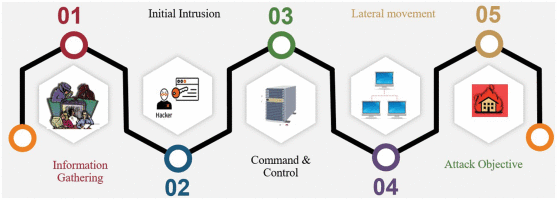
\includegraphics[width=1\textwidth]{UWThesis/images/apt_malware.png}
\caption{APT Malware Exploitation Phases}
\label{sec:apt_malware_flow}
\end{figure}

\section{Objective}
This project develops an endpoint-centric security framework to prevent DNS-based data exfiltration in real time across distributed Linux systems. By embedding detection and enforcement logic directly in the kernel using eBPF, the system targets covert C2 implants, DNS tunneling, and obfuscated payloads—delivering rapid threat response, deep visibility, and zero-trust enforcement across distributed environments.


% \section{Objective}
% This project develops a security framework to proactively prevent various forms of data exfiltration over the DNS protocol, with a specific focus on endpoint-based enforcement in Linux systems and distributed  environments. The system targets a broad range of threats, including low-throughput DNS exfiltration via beaconing implants, high-throughput DNS data breaches, and DNS tunneling, even when encapsulated over nonstandard ports. By embedding detection and prevention logic directly into the Linux kernel using Extended Berkley Packet Filter (eBPF), the framework enables termination of malicious DNS C2 implants at the lowest layer of the operating system. It is tightly integrated with the kernel syscall layer to reduce attacker dwell time and enable real-time response. The framework incorporates rich lexical analysis to detect obfuscated DNS payloads and uses deep learning models trained on large datasets of malicious traffic to enhance detection accuracy while minimizing false positives. It also enforces strict privilege separation between userspace and kernel space using Linux Security Modules (LSM) and seccomp, following the principles of least privilege and zero trust. This system is designed to counter domain evasion techniques such as Domain Generation Algorithms (DGA), randomized beaconing intervals, and encapsulated payloads, while also producing actionable telemetry and observability for tracing and incident response of DNS-based threats in distributed environments.
% By combining advanced Linux kernel programming (v5.2+), deep learning–assisted threat detection, and real-time security enforcement in distributed systems over DNS servers, the project addresses a critical gap in securing DNS which both research and enterprise security solutions lack.

\chapter {Background}
\section{eBPF}
Extended Berkeley Packet Filter (eBPF) was introduced in Linux kernel version 3.15 (2014) as a general-purpose in-kernel virtual machine. It evolved from classic BPF \cite{10.5555/1267303.1267305}, which was originally limited to packet filtering through a domain-specific language and lacked the flexibility for injecting custom logic into the kernel. Unlike kernel modules, which can destabilize the system, eBPF enables safe, dynamic programmability by injecting verified code into the kernel without compromising stability or security. eBPF programs are written in a restricted subset of C, compiled to eBPF bytecode using LLVM, and executed by the in-kernel eBPF virtual machine. These programs operate under a strict execution model: a RISC-like instruction set, eleven 64-bit general-purpose registers, a 512-byte stack, and a hard cap of one million instructions. The bytecode is architecture-agnostic, making it portable across hardware platforms running the Linux kernel. To further support compatibility across different kernel versions, eBPF uses BPF Type Format (BTF) to encode type information, enabling introspection, debugging, and safe reuse of eBPF programs across different kernel versions. Before execution, the kernel’s BPF verifier statically analyzes the bytecode to ensure memory safety, bounded loops, and control flow integrity. This strict verification model makes eBPF an ideal foundation for in-kernel security applications, mitigating risks from malicious code while ensuring system stability. In addition, eBPF programs are JIT-compiled, minimizing performance overhead. Because eBPF programs run in a sandboxed kernel environment, they can safely access internal kernel subsystems, which is particularly useful for security sensitive programs requiring low-level inspection of networking stacks or access to the Linux Security Module (LSM) layer. A key strength is the use of eBPF maps: persistent, kernel-resident key value stores that support various data structures (e.g., stacks, queues, LRU caches). These maps enable stateful security applications to share data between userspace and the kernel, persist state across program lifetimes via pinning to the BPF virtual filesystem, and dynamically reprogram kernel behavior at runtime, particularly valuable for eBPF programs that enforce adaptive security policies in coordination with advanced userspace analysis. All interactions with eBPF—program loading, unloading, and map management—are performed via the bpf() syscall, typically restricted to privileged users with \texttt{CAP\_BPF} or \texttt{CAP\_SYS\_ADMIN} to reduce the attack surface. This architecture makes eBPF a powerful foundation for building advanced security enforcement frameworks, especially for detecting and mitigating data exfiltration, while still supporting deep observability, fine-grained tracing, and real-time in-kernel policy enforcement. The \hyperref[fig:eBPF-injection]{Figure 2.1} below outlines the four key phases of an eBPF program’s lifecycle—development, compiling, loading, verifying and monitoring, and runtime attachment—specifically in the context of monitoring socket\_write operations initiated by userspace processes.

 % Once verified, the kernel can further optimize the program using in-kernel Just-In-Time (JIT) compilation, benefiting from both LLVM optimizations during compilation and runtime JIT enhancements after attachment. eBPF programs interact with userspace via maps—persistent, kernel-resident key-value data structures. These maps allow secure sharing of state and come in various types optimized for different use cases, such as BPF\_MAP\_TYPE\_LRU\_HASH, BPF\_MAP\_TYPE\_LPM\_TRIE, and BPF\_MAP\_TYPE\_STACK. Maps can be accessed using a map ID or a pinned file descriptor through the BPF virtual file system, enabling persistence beyond the lifetime of the original userspace loader.Program loading and interaction are tightly controlled through a single syscall: bpf(). Kernel-level Mandatory Access Control and Linux capabilities (e.g., CAP\_BPF, CAP\_NET\_ADMIN) are enforced to reduce the attack surface. For instance, attaching eBPF programs to the network data path requires CAP\_NET\_ADMIN, especially when managing network interfaces via AF\_NETLINK sockets. Once injected, eBPF programs are attached to various kernel hook points—network stack, scheduler, security modules—using kernel probes, tracepoints, or userland hooks.

\label{sec:ebpf-inject-flow}
\begin{figure}[h]
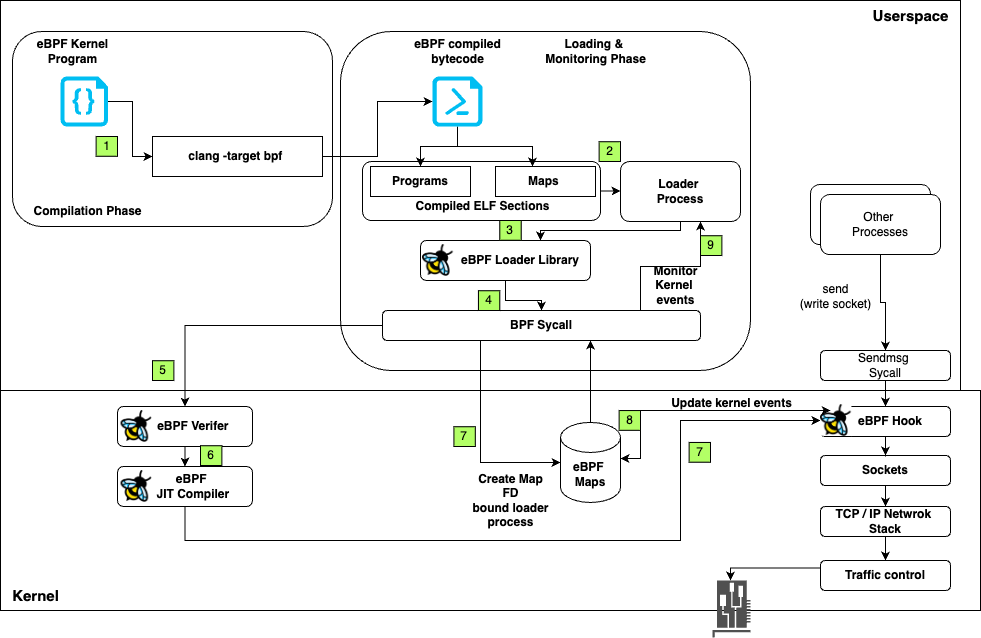
\includegraphics[width=0.9\textwidth]{UWThesis/images/eBpf inject flow.png}
\caption{eBPF Programs Injection Phases in Kernel}
\label{fig:eBPF-injection}
\end{figure}

\newpage
\section{Linux Kernel Network Stack}
The Linux kernel network stack refers to the sequence of processing steps that network packets follow as they traverse the kernel’s networking stack in both the incoming (ingress) and outgoing (egress) directions. Each packet in kernel network stack represented as SKB (socket kernel buffer), a fundamental data structure used to represent packets in memory. Each SKB acts as a metadata-rich container, implemented as a linked list, allowing the kernel to manipulate packets as they move through different layers of the stack by sliding SKB head pointer over SKB data associated head pointers . Every packet—whether entering or leaving the system—passes through multiple processing stages. These include scheduling, classification, filtering, shaping, and forwarding. The datapath handles these operations across various network interfaces, or \texttt{netdevs}, which are kernel abstractions for hardware or virtual network devices. In both ingress and egress directions, packets are managed through dedicated queues, either software-based or hardware-backed, depending on the NIC and driver implementation \cite{stephan2024path}. The egress flow is particularly important for detecting and preventing data exfiltration, as malicious packets typically originate from compromised userspace processes. Once a userspace application writes data to a socket, the kernel routes this packet through several stages: the socket layer (TCP/IP stack), the Netfilter subsystem (link layer), the traffic control (TC) system for shaping and classification, and finally to the device driver that transmits the packet through the NIC firmware as illustrated \hyperref[sec:kernel-network-datapath]{Figure 2.2}.

% \begin{itemize}
%     \item \textbf{Socket Layer}: Interfaces with userspace and manages TCP/IP protocol socket types.
%     \item \textbf{Netfilter (Link Layer)}: Processes netdev flows and provides basic packet manglineg/filtering capabilities.
%     \item \textbf{Traffic Control (TC)}: Implements Quality of Service (QoS), traffic shaping, and classification via the classful or classles queuing discipline (qdisc) system.
%     \item \textbf{Network Device Drivers}: Handle the transmission of packets over physical or virtual interfaces.
% \end{itemize}
% Linux supports both software-based and hardware-based netdevs, each with dedicated drivers. Communication between userspace and the kernel networking stack is often managed via \texttt{NETLINK} sockets, particularly when configuring subsystems like TC or Netfilter.

\label{sec:kernel-network-datapath}
\begin{figure}[h]
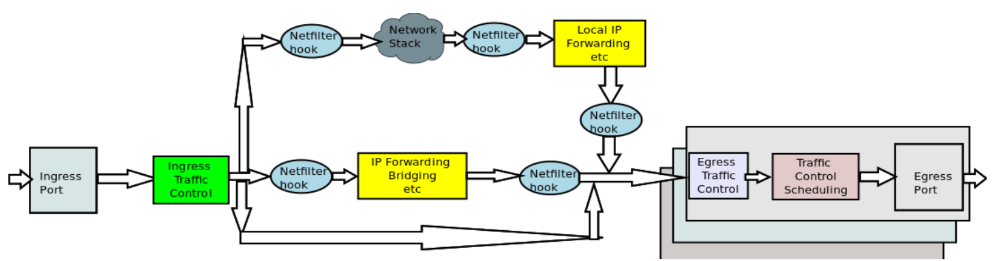
\includegraphics[width=1.0\textwidth]{UWThesis/images/kernel_datapath_flow.png}
\caption{Linux Kernel Network DataPath}
\end{figure}



\section{eBPF Integration with the Linux Kernel Networking Stack}
Among the various subsystems within the Linux kernel network datapath, Traffic Control (TC) is particularly critical for enforcing security in the egress direction, where exfiltration attempts typically occur. TC enables fine-grained control over network traffic through mechanisms such as shaping (rate limiting), scheduling, policing, and filtering. It operates primarily through queuing disciplines (qdiscs)—kernel-level constructs attached to a netdev that define how packets are enqueued, dequeued, and processed before transmission by a network device (TX path steering) \cite{salim2015linux}.
TC supports both classful and classless qdiscs, allowing packets to be classified and processed based on a hierarchy or flat model. Among these, the CLSACT (classless qdisc with actions) discipline plays a unique role. Unlike traditional classful qdiscs, CLSACT is a lightweight, classless metadata qdisc still supporting RX, TX software queues, max length like other classful qdisc that can be attached on top of both classful (e.g., HTB) and classless (e.g., MQ\_PRIO, FQ\_CODEL, MQ\_CAKE) qdiscs allowing both packet classification and implementing packet forwarding actions post classification all inside single QDISC. The CLSACT QDISC enables priority-based attachment of multiple filters to a network device, allowing a complete in-kernel traffic filtering chain using TC. Its primary advantage lies in the ability to attach eBPF programs as filters, enabling the execution of custom logic directly within the kernel before any action is taken. CLSACT supports both ingress and egress paths, allowing eBPF programs to process netflows with defined priorities. This enables DPI and fine-grained security enforcement without modifying the device’s queuing behavior or requiring changes to existing qdiscs \cite{borkmann2016getting}. 
eBPF programs attached via CLSACT execute on every packet passing through the hook prior to any default QDISC present on the netdev, enabling real-time inspection, advanced custom packet filtering compared to legacy TC packet classifer for other QDISC's which have different components for classification and actions.  This makes it particularly well-suited for DNS data exfiltration prevention, where enforcement needs to happen before the packet lands over NIC driver queues. The CLSACT qdisc is widely leveraged by Container Network Interface (CNI) plugins in orchestration environments like Kubernetes for overlay networking and node-to-node communication. However, its potential for enforcing in-kernel security policies—particularly for preventing data breaches—remains largely untapped. Moreover, eBPF can also be attached kernel link layer (netfilter), sockets, and finally over kernel's mandatory access control and syscall layer. 
This broad hook coverage allows eBPF to power everything from performance profiling, network observability, and rate limiting to runtime threat detection, load balancing, and deep in-kernel packet inspection, all with the utmost security. \hyperref[sec:ebpf-hooks-kernel-network-datapath]{Figure 2.3} illustrate the various attachment points within the kernel network stack for in-kernel programmability.
% used in scalable security architectures primarily for bandwidth, and throughput measurement, rate limiting, or packet mangling however, supporting actions over packet post-classification this QDISC IS extensively useful for packet filtering in the kernel TC layer based packet payload characteristics

% intercept packets just before transmission or immediately after reception, enabling drops, header rewrites, metadata tagging, and rerouting to different netdevs, all from inside the kernel.
% Beyond TC, the deep integration of eBPF with the Linux networking stack allows injection of advanced security logic per packet at multiple strategic hook points: \hyperref[sec:ebpf-hooks-kernel-network-datapath]{eBPF hooks} explains all eBPF different hook points in the kernel network data path. In addition, with faster packet processing socket types introduced in linux kernel (AF\_XDP) allows injection of raw packets directly from userspace into the device driver TX queues, allowing fast egress packet processing by passing kernel network stack particularly highly relevant for high egress packet processing.

% \begin{itemize}
% \item \textbf{XDP (Express Data Path)}: Executes at the earliest ingress point, in the NIC driver, before the kernel allocates memory for the packet.
% \item \textbf{Traffic Control (TC)}: Executes at both ingress and egress via clsact, allowing programmable filtering on sk\_buff structures.
% \item \textbf{Socket Layer and CGroups}: Enables filtering and accounting at the socket API level, with namespace and container awareness.
% \item \textbf{Netfilter and LSM}: Interfaces with iptables/nftables and Linux Security Modules for netdev link, kernel mandatory access control for certain kernel syscalls.
% \item \textbf{Raw Tracepoints and KProbes}: Instrument arbitrary kernel functions for tracing, introspection, or runtime logic injection.
% \end{itemize}


% While cloud native environments such as Kubernetes have adopted eBPF through CNIs like Cilium (from Isovalent, now part of Cisco) for enforcing L3/L7 policies and observability, current solutions focus largely on kernel socket layer for filtering, load-balancing or DDoS prevention via XDP. To date, no industry solution has comprehensively leveraged eBPF across the Linux network stack, syscall interface, and security subsystems to proactively prevent DNS exfiltration or disrupt active Command-and-Control (C2) activity in real time.




\begin{figure}
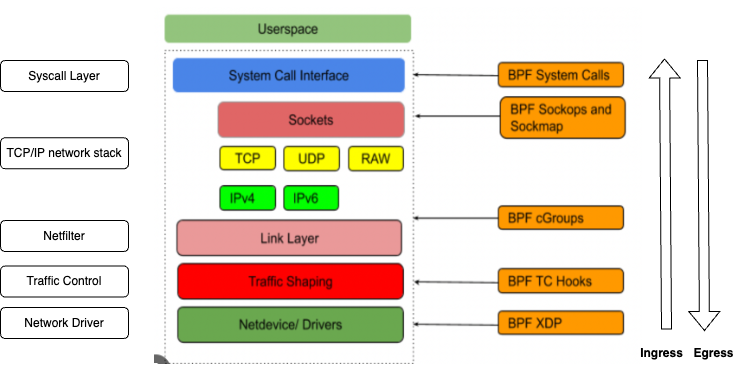
\includegraphics[width=1.0\textwidth]{images/kernel_datapath.png}
\caption{eBPF hooks over Linux Kernel Data Path}
\label{sec:ebpf-hooks-kernel-network-datapath}
\end{figure}


\section{DNS-based Data Exfiltration}
DNS data exfiltration is a distinct category of data breaches where sensitive information is stealthily extracted from corporate networks via the DNS protocol. This technique is typically carried out by remote-controlled, fileless malware implants that operate entirely in memory, leaving minimal forensic footprint on infected endpoints. DNS-based exfiltration exploits the protocol’s ubiquity and inherent trust to covertly transmit stolen data—either as raw payloads or tunneled traffic from blocked protocols—by encoding it into the subdomain portion of DNS queries. \hyperref[dns_payload_obfuscation]{Table 2.1} details some of the most widely used payload obfuscation techniques to encode DNS exfiltrated data. These queries follow the standard hierarchical resolution path and ultimately reach attacker-controlled domains or delegated nameservers. Adversaries leverage DNS for data exfiltration by encoding small chunks of data across multiple queries using common query types such as \texttt{A}, \texttt{AAAA}, \texttt{MX}, \texttt{SRV}, and \texttt{HTTPS}, or by utilizing record types that support arbitrary payloads, including \texttt{TXT} and \texttt{NULL}. These latter types are frequently used in payload-based exfiltration, allowing queries to contain non-DNS data. In command-and-control (C2) scenarios, attackers can issue commands via DNS responses, with \texttt{TXT} and \texttt{NULL} records serving as flexible data containers. These mechanisms allow attackers to disguise and transmit sensitive information through traffic that appears benign. To evade detection, adversaries employ techniques such as randomized query intervals, encryption with ephemeral keys, and domain generation algorithms (DGAs) that rotate second-level domains. Advanced implants may also tunnel non-DNS Layer 7 (L7) protocols over DNS, leveraging arbitrary Layer 4 (L4) ports beyond the standard ones (e.g., 53, 853, 5353) as done by DNSCAT2 adversary emulation framework for data exfiltration, complicating both traffic analysis and firewall-based centralized passive monitoring solutions deployed in distributed environments.
\hyperref[sec:dns c2 flow]{Figure 2.4} explains phases of carrying out DNS data exfiltration.
The three primary forms of DNS-based exfiltration—tunneling, raw exfiltration, and command-and-control (C2) channels—are described in the subsections below.

\begin{table}[H]
\centering
\begin{tabular}{|l|l|l|}
\hline
\textbf{Encoding Format} & \textbf{Exfiltrated Payload} & \textbf{Encoded DNS Subdomain} \\
\hline
Base64 & TopSecret & VG9wU2VjcmV0.dns.exfil.com \\
\hline
Mask (XOR 0xAA) & TopSecret & DE.D5.F2.F9.E9.C7.CF.DE.dns.exfil.com \\
\hline
NetBIOS & TopSecret & ECPFEDFEFCDCECEEEA.dns.exfil.com \\
\hline
CRC32 (Hex) & TopSecret & 7F9C2BA4.dns.exfil.com \\
\hline
AES-CBC (Hex + IV) & TopSecret & IV.A1.B2.C3.D4.E5.F6.07.08.dns.exfil.com \\
\hline
RC4 (Hex) & TopSecret & 9A.B3.47.E2.8C.4D.11.6F.dns.exfil.com
\\
\hline
Raw (Hex) & TopSecret & 546f70536563726574.dns.exfil.com
\\
\hline
\end{tabular}
\caption{DNS Payload Obfuscation Techniques}
\label{dns_payload_obfuscation}
\end{table}

\subsubsection{DNS Tunneling}
DNS tunneling abuses the protocol to encapsulate arbitrary data or non-DNS payloads within query fields, allowing attackers to bypass firewalls and traditional perimeter defenses. By disguising malicious payloads as legitimate DNS traffic or blending with benign traffic, it enables covert bidirectional communication between compromised systems and remote servers. Tunneling may operate in low- or high-throughput modes, with traffic patterns modulated to evade anomaly-based detection systems.
Sophisticated variants exploit kernel-level encapsulation methods (e.g., \texttt{TUN/TAP}, VXLAN) using virtual interfaces. While these methods require elevated privileges (e.g., \texttt{CAP\_NET\_ADMIN}), the sporadic nature of encapsulated traffic makes detection through passive monitoring particularly challenging.

\subsubsection{DNS Command and Control (C2)}
DNS-based C2 is an advanced form of tunneling that establishes persistent, covert channels between implants and attacker infrastructure. Malicious implants use DNS queries to poll for encoded instructions and execute responses—forming full-duplex control channels. These channels can shift between rapid polling and low-frequency beaconing to remain stealthy. Some C2 channels leverage cross-protocol communication, use rotating IPs, and integrate domain generation algorithms to evade static detection.
Conventional defenses such as static blacklists and rule-based systems are ill-suited to counter these dynamic threats. Early-stage detection and endpoint-level disruption are critical, as even brief persistence can result in data loss and lateral movement. Currently, no known research or proprietary solutions offer real-time termination of both the DNS C2 channel and the associated implant process at the endpoint—especially before any command execution or exfiltration occurs.

\subsubsection{DNS Raw Exfiltration}
Raw exfiltration over DNS involves directly leaking files or sensitive data in high-volume bursts of DNS queries over a short duration. While this method often creates detectable spikes in traffic, it can still succeed before monitoring systems trigger alerts or enforcement kicks in. Most existing solutions rely on passive network monitoring and cannot guarantee zero or near-zero data loss.
Real-time prevention—prior to transmission—is essential, especially when exfiltration bypasses traditional IDS systems. Unlike tunneling or C2, raw exfiltration is typically unidirectional and lacks duplex communication. Instead, it focuses solely on stealthily transferring obfuscated data through common DNS query fields such as subdomains, often using base32/base64 encodings and chunked transmissions to bypass protocol validation layers.


\label{sec:dns c2 flow}
\begin{figure}[h]
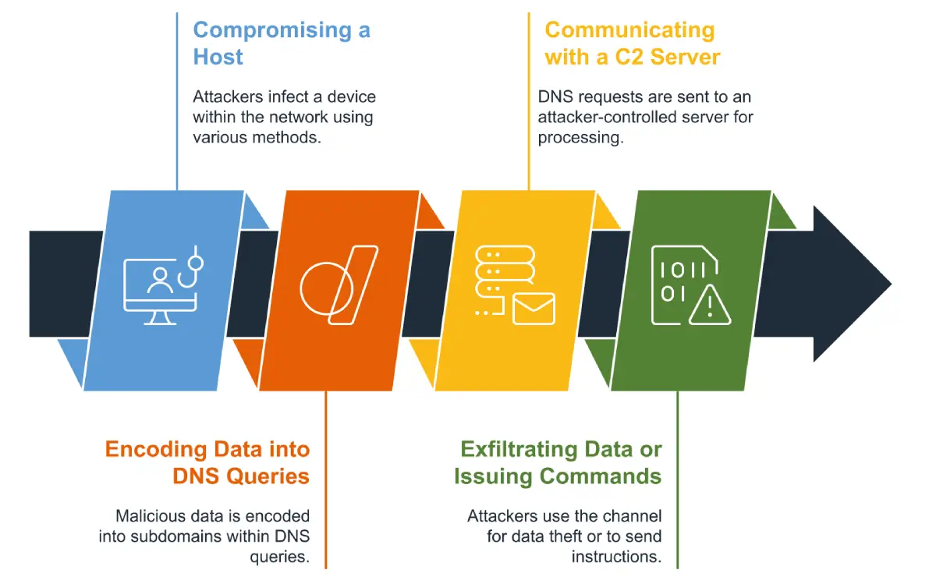
\includegraphics[width=1\textwidth]{UWThesis/images/dns_exfil_flow.png}
\caption{DNS Data Exfiltration Phases}
\end{figure}



% \section{DNS protocol transport enforcements}
% The DNS protocol, as originally specified in RFC 1035, was not designed with security in mind. It imposes several structural limitations designed to reduce complexity and overhead in early network environments. By default, DNS uses UDP as its transport protocol, restricting the payload to 512 bytes per query or response. With the introduction of EDNS0 (Extension Mechanisms for DNS), this limitation was relaxed to allow UDP payloads up to 4096 bytes, enabling support for modern features such as DNSSEC. In addition, DNS also supports for transport over TCP for larger payload sizes. As a protocol level enforcement DNS domain names are limited to 255 characters in total length, composed of a maximum of 127 labels / octets, with each label being no more than 63 characters. 
\section{DNS Security Enhancements and Their Limitations}
Several protocol-level security enhancements have been proposed and standardized to strengthen DNS integrity and privacy. These include:
\begin{itemize}
    \item DNSSEC: Adds cryptographic signatures to DNS records to ensure authenticity and prevent spoofing or cache poisoning. However, DNSSEC does not provide encryption or confidentiality, leaving the DNS payload visible to any intermediate observer. As such, it offers no protection against covert channels or data exfiltration mechanisms embedded within legitimate-looking queries.
    \item DNS-over-TLS (DoT) and DNS-over-HTTPS (DoH): Encrypt DNS queries to prevent surveillance and man-in-the-middle attacks. While effective at improving privacy, this encryption also impairs traditional security tools from performing deep packet inspection (DPI) on DNS traffic encapsulated within TLS or HTTPS. This blinding effect weakens intrusion detection systems (IDS) and data loss prevention (DLP) tools.
\end{itemize}
Although these enhancements protect against certain classes of attacks, none are designed to prevent data exfiltration through DNS, particularly when it originates from implants on the endpoint that abuse protocol-compliant structures for covert communication.

\section{Existing Prevention Mechanisms and Their Limitations}
To date, the most widely deployed preventive mechanisms for DNS-based exfiltration include:
\begin{itemize}
\item \textbf{DNS Sinkholing}: Redirects queries for known malicious domains to controlled endpoints, preventing external resolution.
\item \textbf{Response Policy Zones (RPZ)}: Enable DNS servers to enforce custom filtering policies based on domain patterns or IP addresses.
\end{itemize}
While these techniques effectively block malicious domains using declarative policies or access control lists to protect internal networks, they remain fundamentally reactive. Most rely on static blacklists generated after detection via intrusion alerts or passive deep packet inspection. As a result, DNS-based data exfiltration or malicious commands over DNS C2 channel can succeed before server rules are updated and enforced. In addition, these methods are not equipped to stop C2 implants that use domain generation algorithms (DGA) to mutate Layer 3 IP addresses and Layer 7 domain names, causing damage before filtering policies can adapt due to the persistent and evolving nature of C2 infrastructure.


% \section{DNS Resolution Flow and Kernel Interaction on Linux}
% The standard DNS resolution flow on Linux involves several user and kernel space components. When a client application initiates a DNS query using functions such as \texttt{getaddrinfo()} via \texttt{libc}, it typically communicates over D-Bus with \texttt{systemd-resolved}, the stub resolver. The \texttt{nsswitch.conf} file defines the order and method of name resolution, whether via DNS, /etc/hosts, or other mechanisms. When the stub resolver is enabled, most systems proxy DNS requests over the loopback interface (usually \texttt{127.0.0.53}). If a DNS response is not found in the local cache, the stub resolver forwards the query to an upstream resolver associated with the physical network interface, using destination NAT (DNAT) and source NAT (SNAT) rules as needed.
% In systems without a stub resolver, DNS queries are sent directly to the upstream resolver via the active \texttt{net\_device}, as managed by \texttt{systemd-resolved}. This routing decision is typically based on default routes assigned through DHCP or static configuration.
% From a kernel perspective, the network device (\texttt{net\_device}) involved in the resolution process determines the interface through which DNS traffic is forwarded. The kernel routes the packet toward the upstream DNS IP address configured in \texttt{/etc/resolv.conf}, based on routing tables and device status. This tight coupling between the resolution process and the kernel network stack is leveraged by the eBPF node agents for inline DNS parsing and enforcement.


\chapter {Related Work}
\section{Network Security using eBPF}
eBPF has emerged as a critical technology for modern networking, security, and observability in Linux. Its ability to inject safe, verifiable code into the kernel makes it ideal for high-performance, in-kernel programmability without compromising system stability. These features have led to widespread adoption by cloud providers, particularly in large-scale data planes and hyperscalers for traffic filtering and enforcement of declarative network policies across multiple layers of the Linux kernel. Most existing research focuses on the ingress path using XDP (eXpress Data Path), a high-speed packet processing mechanism integrated into network driver firmware. Initially proposed by \citeauthor{10.1145/3281411.3281443}, XDP was later adopted into the Linux kernel to enable early packet drops, hardware offload at the NIC level, and improved throughput. It is often combined with eBPF to support programmable, low-latency network processing and security enforcement for DDoS preventions \cite{10.1145/3281411.3281443, 8850758}.
\citeauthor{10.1145/3371038} studies provide architectural overviews and performance analyses of eBPF in networking contexts \cite{10.1145/3371038}, similarly \citeauthor{bertrone2018accelerating} explains accelerating kernel network firewalls by combining eBPF and iptables \cite{bertrone2018accelerating}, yet they predominantly address inbound traffic. In contrast, the egress path—critical for detecting and preventing data exfiltration remains relatively underexplored. 

% This is particularly relevant for DNS-based exfiltration, which exploits outbound DNS traffic to evade perimeter defenses. The Linux Traffic Control (TC) subsystem provides a suitable hook for egress inspection, allowing eBPF programs to analyze and intercept DNS packets before they leave the host. Leveraging TC in this context enables endpoint-resident, low-level enforcement that is more resistant to evasion.

\citeauthor{9165454} explored DNS-related defenses using eBPF, leveraging XDP to mitigate DNS water torture DDoS attacks by analyzing queries directly at the network interface of authoritative DNS servers \cite{9165454}. While effective for volumetric DDoS mitigation, their approach is limited in scope and does not address low-volume, stealthy data exfiltration. Similarly, \citeauthor{bertin2017xdp} proposed an XDP-based strategy for mitigating ingress-layer DDoS floods, such as TCP SYN and UDP amplification attacks \cite{bertin2017xdp}. However, this technique also falls short in handling sophisticated or covert DNS-based exfiltration threats.
Based on current literature, \citeauthor{steadman2021dnsxp} presents the only as of know eBPF-based system specifically aimed at DNS exfiltration prevention. Their approach combines eBPF and SDN to enforce static rules in the data plane while performing flow analysis in the control plane \cite{steadman2021dnsxp, 8725640}. However, their design attaches eBPF programs at the XDP layer—suitable only for ingress traffic—which limits its effectiveness against exfiltration. Moreover, reliance on static rules increases false-positive rates and restricts adaptability to novel attack patterns. The use of P4 switches and packet mirroring to the SDN controller also introduces latency, hindering real-time enforcement. Moreover, their evaluation was not able to prevent stealthy exfiltration leading to data loss with more stealthy traffic mirroring to control plane. Similarly, enterprise tools such as Isovalent Cilium (now part of Cisco) support eBPF-based Kubernetes network policies at layers L3–L7 \cite{zavarella2022methodology}. While DNS-aware L7 policies allow for domain-level whitelisting, they lack dynamic blacklisting and are not tailored for detecting exfiltration behaviors. Open-source tools like Microsoft’s Inspector Gadget also rely on static rules defined in userspace and do not provide deep, kernel-level enforcement mechanisms. These limitations highlight the need for a comprehensive eBPF-based solution that operates at the egress point and supports dynamic security enforcement not only inside the kernel via eBPF but also in an distributed environment with dynamic domain blacklist to combat DGA. 
% This project addresses that gap by combining deep packet inspection in the kernel with real-time DNS anomaly detection powered by userspace deep learning models. The proposed system enables low-latency, adaptive enforcement against unauthorized DNS communication, directly within the Linux kernel.

\section{Machine Learning for Detecting DNS Data Exfiltration}
Advancements in network security have significantly enhanced the detection of DNS data exfiltration, often leveraging machine learning to analyze packet patterns and payloads. Many solutions combine DPI with anomaly-based analysis of DNS traffic volume and timing, detecting potential exfiltration attempts via DNS firewalls or integrated intrusion detection systems. For C2-based exfiltration, \citeauthor{apt-process} focuses on behavioral analysis, using system resources like PowerShell and Windows backdoors alongside DNS tunneling for APT detection \cite{apt-process}. However, these methods primarily detect exfiltration and fail to fully prevent DNS tunneling, with no clear response time or method for breaking the C2 communication or terminating the implant. Similarly, \citeauthor{Das} proposes a machine learning model that identifies DNS-based data exfiltration using real malware samples from financial institutions, though potential evasion strategies are also discussed \cite{Das}. Meanwhile, \citeauthor{8717806d} suggests a real-time detection mechanism using the Isolation Forest algorithm \cite{8717806d}, but their stateless analysis fails to address protection against prolonged, stealthy APT malware or C2 exfiltration. Several approaches have focused on DNS server-side detection, blending stateful and stateless features. \citeauthor{bilge2011exposure} introduced the EXPOSURE system, which identifies suspicious domains by extracting 15 features from DNS traffic, categorized into query-name, time-based, answer-based, and TTL-based features. Validated using a dataset of 100 billion DNS requests, this system effectively identifies domains involved in botnet C2 and spamming \cite{bilge2011exposure}. However, the system’s focus is on detection rather than prevention, and it is limited by the reliance on passive analysis of DNS queries. Similarly, \citeauthor{antonakakis2010building} proposed NOTOS, a dynamic reputation system analyzing passive DNS queries, extracting 41 features classified into network-based and zone-based categories \cite{antonakakis2010building}. While it identifies malicious domain characteristics, it falls short in detecting data exfiltration and lacks real-time detection capabilities, making it ineffective against stealthy C2-based exfiltration. \citeauthor{DBLP:journals/corr/abs-1709-08395} developed a solution for detecting malicious, low-throughput exfiltration using domain-specific features such as entropy and query time intervals, employing one-class SVM and Isolation Forest. However, their reliance on past traffic limits its real-time detection capabilities \cite{DBLP:journals/corr/abs-1709-08395}. Other studies, such as \citeauthor{10.1145/3230833.3233278}, explore machine learning models for C2 tunneling detection, but their effectiveness is hindered by the inability to detect stealthy C2 over long exploitation periods \cite{10.1145/3230833.3233278}. \citeauthor{9486400} uses mobile agents for real-time detection and mitigation, but the approach is prone to false positives and introduces latency due to agent hops across the network, making it unsuitable for real-time security enforcement \cite{9486400}. While solutions like \citeauthor{haider2024c2}  attempt to address C2-based DNS exfiltration over package distribution systems to prevent supply chain attacks, their approach is efficient for preventing exfiltration from single node but lacks detailed mechanisms for detecting and preventing DNS data exfiltration across multiple nodes or deep system-level observability \cite{haider2024c2,sivakorn2019countering}. These solutions remain vulnerable to policy evasion, privilege escalation, and denial-of-service attacks, largely due to limited kernel integration and insufficient enforcement of security policies. Process DNS, as introduced by \citeauthor{sivakorn2019countering}, focuses on detecting and countering C2-based DNS exfiltration, specifically by analyzing processes in userspace and terminating malicious ones \cite{sivakorn2019countering}. Despite its low-latency detection approach, the solution is vulnerable to privilege escalation and denial-of-service attacks due to its lack of kernel integration and inability to handle more sophisticated evasion tactics. The lack of transparency regarding the kernel enforced system access control mechanisms for their agents in userspace further limits its effectiveness, particularly for advanced threat actors that may bypass userspace defenses.
Existing machine learning–based DNS security solutions primarily focus on volumetric and timing-based anomaly detection, as they are confined to passively analyzing aggregated traffic in userspace. These architectures inherently lack critical capabilities such as real-time enforcement, in-kernel inspection of encapsulated payloads, cross-protocol correlation, and detection of port-layer obfuscation—such as DNS tunneling over randomized UDP ports. They remain decoupled from active prevention, offering no mechanisms for preemptive data loss estimation or dynamic response. Most rely on stateless or stateful analysis and are rarely evaluated against advanced adversary emulation frameworks or modern C2 tools. While lexical inspection can offer fast classification of suspicious payloads, userspace-based systems still depend on behavioral heuristics or statistical timing models to detect slow and stealthy exfiltration, often resulting in substantial data loss before enforcement is applied. Moreover, they are fundamentally incapable of preventing advanced C2 behaviors such as remote code execution, port forwarding, backdoor creation, or reverse shells. Machine learning–driven detection, particularly in passive userspace pipelines, may eventually flag these activities—but only after partial command execution or exfiltration has already occurred, making such defenses reactive and too late to prevent damage. These approaches may be adequate for bulk exfiltration scenarios but consistently fail against sophisticated threats like multi-layered C2, botnets, and domain generation algorithms. Despite incremental advances, no current solution offers true real-time DNS exfiltration prevention with implant-level termination, fine-grained enforcement, and cloud-native scalability. Userspace-only designs fundamentally lack visibility into low-level network activity and cannot introspect system state with sufficient granularity, rendering them ill-suited for production-grade environments where data sovereignty, rapid containment, and kernel-level control are paramount.

\section{Enterprise Solutions to Prevent DNS Data Exfiltration}
Akamai’s ibHH algorithm leverages information heavy hitters for real-time DNS exfiltration detection adopted in production as explained by \citeauthor{ozery2023information} by quantifying unique data transmitted from DNS subdomains to their domains, using a fixed-size cache for efficient processing \cite{ozery2023information}. While DNS firewalls like Akamai and AWS Route 53 can detect tunneling and DGA activity using volume thresholds and anomaly rules, they lack direct endpoint prevention—crucial for minimizing data loss and reducing dwell time. These systems often fail against APT malware employing slow, stealthy C2 patterns, and require static, manual policies that are ineffective against dynamic DGAs. Route 53 also lacks enhanced observability and cross-protocol correlation, limiting its ability to enforce Layer 3 blocks via AWS network firewalls. Similarly, proprietary DNS firewalls from Cloudflare, Akamai, and AWS are optimized for DDoS mitigation but fall short against sophisticated exfiltration or insider threats using DNS-based C2. Infoblox adds hybrid agent-based enforcement and centralized threat intelligence, and Broadcom’s Carbon Black blocks endpoint processes—but both rely on userspace traffic analysis. In contrast, eBPF enables in-kernel enforcement with fine-grained visibility, offering significantly stronger mitigation and detection capabilities for DNS exfiltration \cite{ahmed2019monitoring}.


% ========== Chapter 2
\chapter{Implementation}
This chapter explains the security framework architecture and its individual components—first highlighting the overall framework, followed by a detailed breakdown of each component.
\section{Security Framework Overview}
The security framework implemented for distributed environments using endpoint security approach enables real-time disruption of stealthy DNS C2 channels and DNS tunneling, preventing malicious exfiltrated DNS packets from passing through the endpoint to ensure negligible data loss. It provides robust capabilities for terminating malicious C2 implants, offering deep system observability and cross-protocol protection by dynamically creating in-kernel network policies that block remote C2 server IPs. Designed for massive scalability and production readiness in modern cloud environments, the framework supports threat event data streaming to enable asynchronous communication. This, in turn, allows for horizontal scalability of data plane nodes and addresses DGAs by dynamically blacklisting domains via RPZ directly on the DNS server. 
\subsection{Data Plane}
The data plane consists of eBPF node agents built purely in golang for pure performance, lesser memory footprints and ease of concurrent programming via goroutines and channels. These agents operate in userspace and dynamically inject eBPF program into the kernel’s TC layer at the egress point for all physical network interfaces at the endpoint to perform in-kernel DPI and filter DNS exfiltrated packets transmitted over UDP. The agent also inject other eBPF programs attached  kernel hook points like kprobes (kernel probes) to monitor the creation of new network devices, raw tracepoints to detect process termination, and socket cgroup hooks (for older kernels) to retrieve \texttt{task\_struct} when native \texttt{task\_struct} support is unavailable over root kernel TC programs.  \hyperref[sec:dp_kernel_prog_ty]{Table 4.2} outlines all eBPF programs and their corresponding kernel injection points utilized by the eBPF node agent. Complementing egress filtering, the agents monitor incoming packets at ingress for real-time inference and maintain a userspace LRU cache of blacklisted domains. This cache is shared with eBPF programs via eBPF maps to ensure coordinated filtering and detection across data paths. The node agents support two prevention modes, which can be configured via the eBPF node agent configuration in userspace. A dedicated eBPF map is used to enable or disable either mode when injected into the kernel. By default, both modes are enabled to ensure high security.

\begin{itemize}[itemsep=1pt,parsep=0pt]
    \item \textbf{Strict Enforcement Active Mode}: DNS packets over standard ports (53, 5353, 5355) are scanned in-kernel using eBPF at the TC egress hook. Malicious packets are dropped immediately. If classification exceeds eBPF instruction limits, the packet is redirected to userspace for further analysis. Userspace agent sniffs redirected traffic and checks against the domain blacklist cache or perform ONNX-based deep learning model inference to identify potential payload obfuscation in DNS traffic. Post userspace inferencing benign packets are retransmitted using high-speed socket options like \texttt{AF\_PACKET} or \texttt{AF\_XDP}, while malicious ones are dropped and their domains added to the cache. This mode effectively halts all forms of DNS exfiltration, while also enabling live disruption of C2 communication and, ultimately, termination.
    
    \item \textbf{Process-Aware Adaptive Passive Threat Hunting Mode}: Designed for nonstandard UDP port overlayed with DNS traffic for exfiltration, this mode clones suspicious packets for userspace analysis while allowing the original packet to continue. If found malicious, the associated process is flagged in eBPF maps. Subsequent DNS packets from that process are dropped in kernel effectively breaking C2 implant communication with remote server. Once a configurable threshold is reached, the process is terminated. This mode is highly effective against stealthy exfiltration techniques using C2 implants that employ port obfuscation and DNS layering over random UDP ports. 
\end{itemize}

In addition to DPI, node agents manage network namespaces and virtual bridges using the \texttt{veth} driver. \hyperref[sec:dp_eBPF_agent_net_topology]{Figure 4.1} explains the network topology, which starts with virtual namespaces and the \texttt{veth} bridge driver over the kernel link layer in the datapath. They maintain eBPF map file descriptors to bridge kernel-userspace communication, enabling advanced analysis. The lifecycle of eBPF programs is tied to the agent in userspace, which operates with elevated privileges to interact with the network datapath, syscall layer, and other privileged kernel subsystems. \hyperref[sec:dp_kernel_cap]{Table 4.1} explains the kernel capabilities which the eBPF node agent runs in. Both mode of agent operation support active response mechanisms include malicious process termination when userspace agent detect repeated exfiltration exceeding configured thresholds. Filtering of traffic in kernel is driven by adaptive thresholds values or limits configured in kernel eBPF maps utilized by eBPF programs for filtering traffic post raw parsing DNS protocol from socket buffer. In userspace, the eBPF node agent also loads quantized and serialized ONNX (Open Neural Network Exchange) deep learning models for fast inference, and exports system telemetry metrics to observanblity backend, and threat events to centralized message brokers. All the configuration which the node agents in userspace enforce in kernel programs is completely reprogrammable from control plane.


% \vspace{z}
% \begin{minipage}{\textwidth}
\begin{table}[H]
\centering
\begin{tabular}{|l|p{10cm}|}
\hline
\textbf{Kernel Capability} & \textbf{Description} \\
\hline
\texttt{CAP\_BPF} & Load eBPF, manage maps \\
\hline
\texttt{CAP\_SYS\_ADMIN} & Attach BPF, mount BPF FS \\
\hline
\texttt{CAP\_NET\_ADMIN} & Manage netdev creation and tc/xdp/cgroup filters attachment \\
\hline
\texttt{CAP\_NET\_RAW} & Send/receive raw packets from netdev tap rx queues particularly via AF\_PACKET sockets  \\
\hline
\texttt{CAP\_IPC\_LOCK} & Lock BPF memory \\
\hline
\end{tabular}
\caption{Linux Kernel Capabilities Required for eBPF Node Agent Functionality}
\label{sec:dp_kernel_cap}
\end{table}
% \end{minipage}

\begin{table}[H]
\centering
\resizebox{\textwidth}{!}{%
\begin{tabular}{|p{2.8cm}|p{2.8cm}|p{2.6cm}|p{10cm}|}
\hline
\textbf{eBPF Program Type} & \textbf{Agent Mode} & \textbf{Injection Point} & \textbf{Description} \\
\hline
\texttt{SCHED\_ACT} & Active, Passive & Physical NICs & Performs in-kernel DNS DPI at TC egress. Interacts with maps and redirects packets to userspace or tracks process info based on mode. \\
\hline
\texttt{SCHED\_ACT} & Active & Veth bridge netdev's & Verifies packet integrity using \texttt{skb\_hash} for redirected DNS traffic over namespaces. \\
\hline
\texttt{KPROBE} & Active & Tun/Tap driver kernel functions & Detects virtual device creation to attach DNS filters dynamically. \\
\hline
\texttt{TRACEPOINT} & Passive & \texttt{process\_exit} & Cleans up eBPF maps when flagged processes exit before agent-enforced termination. \\
\hline
\texttt{LSM} & Active, Passive & \texttt{BPF\_PROG\_LOAD} & Intercepts eBPF program loading syscalls. Verifies integrity via kernel keyring to block malicious eBPF code injection. \\
\hline
\end{tabular}%
}
\caption{eBPF Programs Managed by the Node Agent}
\label{sec:dp_kernel_prog_ty}
\end{table}

% start each implementation with component it lies in
\begin{figure}[H]
\centering
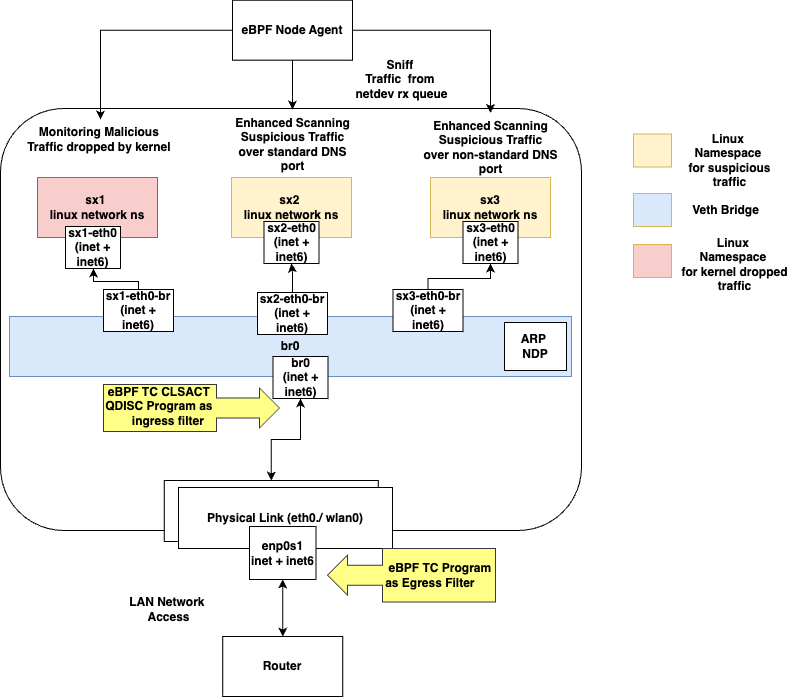
\includegraphics[width=1.0\textwidth]{UWThesis/images/ebpf_network_topology.png}
\caption{eBPF Node Agent created Network Topology at endpoint}
\label{sec:dp_eBPF_agent_net_topology}
\end{figure}

\vspace{-1em}
\subsection{Distributed Infrastructure}
In addition to the data plane nodes, the framework includes an open-source DNS infrastructure built with PowerDNS. The setup consists of a PowerDNS Recursor for upstream resolution and an authoritative DNS server for handling internal zones. While no actual local domains exist, the authoritative server is primarily used to generate malicious C2 domains using a domain generation algorithm (DGA) on a single compromised endpoint within the CSSVLAB environment. This design enables DNS-based C2 and tunneling attacks across the data plane. To support DGA-driven malicious domain generation without relying on public cloud DNS providers, both PowerDNS components were deployed locally. The authoritative server uses a Postgres backend to store DNS zones, records, transfers (AXFR, IXFR), TSIG keys, DNSSEC keys, and related metadata. All data plane nodes are configured to use the PowerDNS Recursor as their default DNS resolver. Kafka acts as a message broker for real-time streaming of threat events detected by eBPF agents in the data plane. To enhance DNS-layer defenses, the framework uses PowerDNS Recursor interceptors to inspect DNS queries before resolution or forwarding. These interceptors perform inference using the same ONNX-serialized deep learning model as the data plane, specifically handling TCP-based DNS queries offloaded from the eBPF agents in data plane. Finally, the recursor is integrated with Response Policy Zones (RPZ), backed by Postgres. These zones are dynamically updated by the controller to blacklist second-level domains (SLDs) tied to malicious C2 activity, as described in the next section.

\vspace{-1em}
\subsection{Control Plane}
The control plane consists of a centralized analysis server that consumes threat events from Kafka topics, streamed and updated by eBPF node agents running in the data plane. Based on these consumed events payloads, the control plane dynamically blacklists malicious SLDs on the DNS server, thereby safeguarding all endpoints in the data plane that utilize the DNS server. Additionally, it fully supports reprogramming the data plane by publishing Kafka topics consumed by node agents, enabling them to rehydrate their local blacklist domain cache and immediately enforce updated policies. This design significantly improves performance for real-time inferencing in userspace.



\section{Data Plane}
The implementation of the eBPF node agents deployed on data plane nodes is organized as follows. First, the \hyperref[sec:active]{active mode} describes the handling of non-encapsulated DNS traffic, detailing the interaction between in-kernel eBPF programs and the userspace node agent. Second, the \hyperref[sec:passive]{passive mode} explains the passive  mode. Third, the \hyperref[sec:encap]{encapsulated phase} outlines the handling of DNS exfiltration over encapsulated traffic, currently supported only in the active phase. Fourth \hyperref[sec:feature]{feature analysis} section covers features extracted by eBPF programs for in-kernel classification, along with userspace feature extraction for deep learning model training and real-time inference on suspicious traffic redirected from the kernel. Fifth, \hyperref[sec:dataset]{dataset} describes the dataset used for model training, and finally, \hyperref[sec:model]{model} details the model architecture, its serialization through ONNX, and quantization for optimized inference performance.


\subsection{Strict Enforcement Active Mode}
\label{sec:active}
After injecting the eBPF programs and attaching them as direct-action filters to the kernel TC egress CLSACT QDISC across all physical network interfaces, the eBPF program is triggered immediately upon packet arrival at the netdev layer. At this stage, inside the QDISC egress filter, the kernel provides a fully formed SKB, which has traversed the upper layers of the kernel network stack and is ready for transmission to the NIC tx queues. The eBPF filter is executed for each packet, with the kernel passing the SKB as input to the filter, and the program runs across multiple CPU cores in parallel. All eBPF maps in this mode are global, and the kernel handles concurrent access to these maps to ensure proper synchronization across cores. First, the \hyperref[sec:dp_eBPF_LRU_Maps_active]{maps} section explains the fundamental structure of the eBPF LRU hash maps used to store state information and manage packet flow.

Next, the netflow across kernel and userspace is explained as follows:
\hyperref[active:sec1]{kernel eBPF filter packet classify}: Describes the packet process and classification on first-time arrival over the TC filter, including actions based on kernel features in the SKB, and handling redirected packets from userspace after timing checks or brute-force verification checks post deep scan. It also details the flow if a packet is found suspicious, including eBPF map updates and redirection to a different veth bridge owned by the eBPF node agent for upstream Linux namespace processing up to userspace and through the kernel network stack.  
\hyperref[active:sec3]{userspace eBPF agent packet handling}: Covers userspace handling of the redirected packet, including sniffing in zero-copy mode.
\hyperref[active:sec3]{Concurrency handling}: Details both userspace and kernel programs concurrency handling over these shared eBPF maps residing in kernel space to userspace eBPF node agent as well as internal synchronization across handled in kernel eBPF programs running these programs over different CPU cores.


% maps definition structure in passive phase 
\begin{figure}[H]
\centering
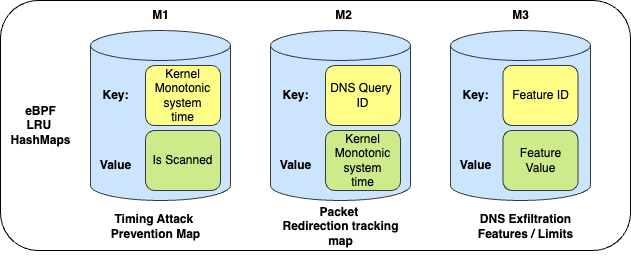
\includegraphics[width=1.0\textwidth]{UWThesis/images/map_struct_port53_active.png}
\caption{eBPF Maps and structure for Node agent in active phase}
\label{sec:dp_eBPF_LRU_Maps_active}
\end{figure}

% eBPF Maps
\subsubsection{\textbf{eBPF Maps in Active mode}}
\begin{enumerate}[itemsep=1pt,parsep=0pt]
\label{sec:maps}
\item \textbf{DNS Exfiltration Feature Map:} \\
Key: Feature identifier \\
Value: Filtering or classification parameter used by the eBPF TC egress program to process DNS traffic.

\item \textbf{Packet Redirection Tracking Map:} \\
Key: DNS query ID \\
Value: Kernel system monotonic time (nanoseconds). Tracks suspicious packets redirected across interfaces, using NMI(Non Maskable Interrupts) safe timestamps.

\item \textbf{Timing Attach Prevention Map:} \\
Key: Monotonic timestamp (nanoseconds) \\
Value: Scanned flag (true/false). Used by the userspace agent to authorize scanned packets, and by the kernel eBPF program to verify packet integrity before resend.
\end{enumerate}



\subsubsection{\textbf{eBPF program packet processing over egress TC QDISC filter}}
\label{active:sec1}
\label{sec:alg1}  
Once a DNS packet traverses down the kernel network stack after being written to the UDP socket by userspace, it reaches the traffic control (TC) layer, with each CPU handling classification and traffic shaping under the parent QDISC of the respective network interface, and before processing any parent QDISC kernel triggers the CLSACT QDISC where the eBPF direct-action filter is attached. At this point, the eBPF program determines whether the packet is arriving for the first time or has been rescanned from userspace by parsing the DNS protocol directly from the kernel SKB. The eBPF program peels off the packet layers from the SKB using the Linux kernel’s core protocol structure definitions, with each protocol layer (L2 to L4) parsed based on the corresponding headers. Since most Layer 7 (application) protocols are handled in userspace, the kernel processes application payloads as raw bytes. Like any other application protocol, DNS also has its protocol header and payload. The eBPF program parses the DNS header from the raw application data using custom written C structure definitions for DNS protcol inside the kernel according to RFC 1035. After populating all required fields like query ID, opcode, flags, question count, and answer count, the eBPF program extracts metadata for further evaluation. If the packet is arriving for the first time, there will be no corresponding entry for its query ID in the \texttt{dns\_packet\_redirection} eBPF map. The TC eBPF program proceeds to parse the DNS application data after the DNS header. It extracts features from the first DNS question; if multiple questions are present, the packet is flagged as suspicious and redirected without further checks, since multiple questions per query are typically disallowed in normal DNS behavior and rejected by most DNS servers. In addition, it is expected that the answer count is zero because the endpoints running these C2 and tunneling implants do not operate full DNS servers and instead communicate with their C2 servers through crafted DNS questions and the additional section of the DNS packet.
These extracted features are evaluated against the kernel feature set described in \hyperref[sec:feature-kernel]{Table 4.3}, and based on the evaluation, appropriate TC actions are enforced, such as \texttt{TC\_ACT\_SHOT} to drop, \texttt{TC\_ACT\_OK} to forward, or \texttt{bpf\_redirect} to redirect the packet to a different network interface. If the packet is benign or malicious the action is taken immediately according to the \hyperref[sec:alg1]{Algorithm 1}. For suspicious packets requiring deeper inspection, before redirection to the different netdev, the parsed DNS query ID is stored as a key in the \texttt{dns\_packet\_redirection} map, with the value being the current kernel system monotonic timestamp obtained via \texttt{bpf\_ktime\_get\_ns}, providing nanosecond precision to accurately track the time of redirection and detect possible timing-based evasion. At this point, additional map information populated by the eBPF node agent in userspace during bootup is fetched, including the recorded L3 address of the bridge interface to which the packet will be redirected, the interface network \texttt{if\_index}, and other system observability maps. Redirection counters are also incremented for the eBPF node agent to export system observability metrics. Prior to redirection, the eBPF program determines whether the incoming packet is IPv4 or IPv6; if IPv4, the program performs destination NAT (DNAT) inside the kernel to modify the L3 destination address and incremental checksum calculation for Ipv4 packets to point to the userspace-owned bridge for inspection, while for IPv6, due to the absence of an L3 checksum in protocol, a static checksum is assigned to maintain consistency. The suspicious packet is then redirected to the RX queues of the associated netdev owned by the userspace eBPF node agent. When the userspace node agent completes deeper inspection and sends the packet back through an AF\_PACKET socket, the TC eBPF program is retriggered. To prevent infinite loops or reprocessing of malicious resends, the eBPF program reparses the DNS protocol from the SKB, fetches the associated timestamp from the \texttt{dns\_packet\_redirection} map using the DNS query ID as key, and retrieves the scan verification flag from the \texttt{dns\_redirect\_ts\_verify\_map}. If the flag is set, authorizing the packet as legitimately scanned and returned by the userspace agent, the packet is forwarded toward the NIC and exits the kernel. If the flag is unset, suggesting the packet is forged, unsanctioned, or a result of a timing or brute-force attack by a compromised implant in userspace, the packet is dropped immediately by the eBPF program. The detailed algorithm for active redirection timestamp handling and userspace resend verification are described in \hyperref[sec:alg2]{Algorithm 2}. Through strict enforcement of privileged map access and precise use of the kernel monotonic clock, the system robustly prevents timing attacks, brute-force attempts, and unauthorized packet exfiltration while deep inspection is performed on the packet, involving context switching between user space and kernel space.



\subsubsection{\textbf{Userspace eBPF Node Agent packet processing}}
\label{active:sec2}
The userspace eBPF node agent utilizes kernel BPF bindings to abstract raw BPF syscalls, primarily through libbpf. The loader runs with the required kernel capabilities as explained earlier, injecting all eBPF programs and owning the file descriptors for eBPF maps both for pinned and unpinned maps to BPF kernel filesystem. It injects the root eBPF program powering the TC filter attached to the egress direction. The agent spawns threads to continuously sniff traffic from its owned network namespace dedicated to handling redirected suspicious traffic in active mode using \texttt{AF\_PACKET} sockets, reading directly from tap interfaces or RX queues in zero-copy mode to avoid additional buffer allocations in userspace for performance. Since the agent has access to all eBPF maps via their file descriptors, it relies on pcap, an extension of libpcap, to parse DNS application-layer traffic redirected from the kernel for inspection. After sniffing, the agent extracts userspace DNS features as outlined in \hyperref[sec:feature-userspace]{Userspace Features}. It maintains two LRU caches in userspace heap memory: first representing Cisco's data set of the world's top one million SLDs, and second representing malicious domains previously inferred and cached, preventing reinferencing known malicious packets. If the parsed SLD is found in the benign cache, the packet is immediately forwarded without inference; due to DNS protocol properties, malicious C2 servers cannot redirect these legitimate domain zone files of the highest-reputed benign domains. The agent forwards benign packets through \texttt{AF\_PACKET} or \texttt{AF\_XDP} sockets accordingly. The agent also supports live Kafka consumers, enabling dynamic updates to the userspace LRU caches from a controller in real time supporting eBPF node agent re-programmability from controller. For AF\_XDP sockets, packets are injected directly into the TX queues of the device driver, bypassing the eBPF TC egress filter, while cleaning up associated entries in the \texttt{dns\_packet\_redirection\_map} added during redirection. For \texttt{AF\_PACKET} sockets, the agent fetches the kernel redirection timestamp using the parsed DNS transaction ID, updates the \texttt{dns\_redirect\_ts\_verify\_map}, and marks the packet as scanned so the kernel allows it to pass. If no cache hit occurs, features are extracted live from the packet and passed to the deep learning model; if the packet is inferred as malicious, it is dropped, the corresponding SLD is blacklisted in the userspace malicious cache, and a Kafka event is produced for the controller to update DNS server blacklists. If benign, the packet is resent using the same approach as a benign cache hit. All malicious detection events are exported to Prometheus along with system observability metrics like redirection counts. The userspace agent continuously monitors maliciously detected packets and the parent processes involved in sending these packets, aided by the same eBPF program that tracks all redirected suspicious DNS packets and their query IDs. If these packets exceed a defined malicious threshold, the userspace agent sends a SIGKILL signal to the process, effectively terminating the malicious implant at the endpoint.
\hyperref[sec:alg3]{Algorithm 3} details the packet processing algorithm utilized by the userspace agent.


\subsubsection{\textbf{eBPF Maps concurrency handling}}
\label{active:sec3}
The eBPF programs in this mode use global kernel maps (not per-CPU) to support concurrent reads/writes, protected by BPF spinlocks NUMA-aware for SMP, extensions of kernel spinlocks that ensure cache coherence and atomic access per CPU. Each map tracks atomic reference counts for process access. Every concurrent thread in usesrpaace processing and sniffing packets parallely from network namespace and if performing updates over shared eBPF map always use RWMutex in userspace for synchronization Since eBPF map fd's are not shared across userspace processes, the maps are exclusively owned by the single eBPF node agent process in userspace ensuring reference count for all the owned map from being garbage collected. This model, paired with spinlock-based concurrency in the kernel per CPU, ensures consistent parallel packet processing across CPUs. The two primary maps shared between kernel and userspace—\texttt{dns\_redirect\_ts\_verify\_map} and \texttt{dns\_packet\_redirection\_map} each of them always using unique keys (monotonic timestamps and DNS query IDs), preventing stale reads, race conditions, and inconsistent updates that could otherwise cause leaking malicious exfiltrated packets. In addition every update done over eBPF maps in the kernel is performed via built-in LLVM concurrency helpers to ensure strong atomic map updates synchronizing kernel memory address locations for map updates. Thus, strict and reliable control is maintained. The \hyperref[sec:dp-active-phase]{Figure 4.3} details the full userspace and kernel pipeline for this mode of agent operation. 

% % alg 1
% \enlargethispage{4\baselineskip}
\begin{algorithm}[H]
\caption{\small DNS RAW SKB Parsing over Egress TC CLSACT QDISC in \textbf{ACTIVE} Mode}
\label{sec:alg1}
\SetKwInOut{Input}{Input}
\SetKwInOut{Output}{Output}

\small % Reduce font size for the entire algorithm
\setstretch{0.9} % Reduce line spacing for more compactness

\Input{Socket buffer (\texttt{skb}), eBPF LRU hash maps: \texttt{dns\_limits}, \texttt{dns\_packet\_redirection}, \texttt{node\_agent\_config}}
\Output{
 \quad Packet Action: \texttt{TC\_ACT\_SHOT}, \texttt{TC\_ACT\_OK} \\ 
 \quad eBPF Map Updates \texttt{bpf\_map\_updates} 
}

\tcp{Parse skb layers; ensure skb->data\_ptr remains memory bound for eBPF verifier}
Parse Layer 2 (Ethernet) from \texttt{skb}\;
\If{VLAN (\texttt{802.1Q} or \texttt{802.1AD}) is present}{
    \If{\texttt{skb->data\_ptr} exceeds \texttt{skb->data\_end}}{
        Drop packet via \texttt{TC\_ACT\_SHOT}\;
    }
    Extract the inner encapsulated protocol (\texttt{h\_proto}) from VLAN header\;
}
Parse Layer 3 (Network) from \texttt{skb}\;
\If{\texttt{skb->data\_ptr} exceeds \texttt{skb->data\_end}}{
    Drop packet via \texttt{TC\_ACT\_SHOT}\;
}
Parse Layer 4 (Transport) from \texttt{skb}\;
\If{\texttt{skb->data\_ptr} exceeds \texttt{skb->data\_end}}{
    Drop packet via \texttt{TC\_ACT\_SHOT}\;
}
\If{\texttt{skb->protocol} = IPPROTO\_TCP}{
    Forward packet via \texttt{TC\_ACT\_OK}\;
}

% Step 1: Extract DNS Header Fields
Parse Layer 7 DNS (Application) from \texttt{skb}\;
\If{\texttt{skb->data\_ptr} exceeds \texttt{skb->data\_end}}{
    Drop packet via \texttt{TC\_ACT\_SHOT}\;
}
Extract \texttt{qd\_count}, \texttt{ans\_count}, \texttt{auth\_count}, and \texttt{add\_count}\;

% Step 2: Header Anomaly Check
\If{\texttt{qd\_count} $>$ 1 \textbf{or} \texttt{auth\_count} $>$ 1 \textbf{or} \texttt{add\_count} $>$ 1}{
    Perform \texttt{bpf\_map\_updates}\;
    \Return\;
}

% Step 3: Parse Question Record and Fetch Limits
Parse first question record from \texttt{skb}\;
\tcp{Extract Kernel DNS features from dns\_limits map}
Fetch \texttt{n\_lbls}, \texttt{dom\_len}, \texttt{subdom\_len}, \texttt{dom\_len\_no\_tld}, \texttt{q\_class}, \texttt{q\_type} from \texttt{dns\_limits}\;

% Step 4: Label Count Check
\If{\texttt{n\_lbls} $\leq$ 2}{
    Forward packet via \texttt{TC\_ACT\_OK}\;
    \Return\;
}

% Step 5: Label and Domain Length Checks
\If{
    Any of (\texttt{n\_lbls}, \texttt{dom\_len}, \texttt{subdom\_len}, \texttt{dom\_len\_no\_tld}) is in [min, max] range
}{
    Perform \texttt{bpf\_map\_updates}\;
    \Return\;
}

\If{
    Any of (\texttt{n\_lbls}, \texttt{dom\_len}, \texttt{subdom\_len}, \texttt{dom\_len\_no\_tld}) exceeds its maximum threshold
}{
    Drop packet via \texttt{TC\_ACT\_SHOT}\;
    \Return\;
}

% Step 6: QTYPE Filtering
\If{\texttt{q\_type} $\in$ \{\texttt{TXT}, \texttt{ANY}, \texttt{NULL}\}}{
    Perform \texttt{bpf\_map\_updates}\;
    \Return\;
}

% Step 7: Default Case
Forward packet via \texttt{TC\_ACT\_OK}\;

\end{algorithm}

% alg 2
\begin{algorithm}[H]
\caption{DNS eBPF Map Handling Prior to \texttt{skb\_redirect} and Post-Socket Write over \texttt{AF\_PACKET} from userspace in \textbf{ACTIVE} Mode}
\label{sec:alg2}
\SetKwInOut{Input}{Input}
\SetKwInOut{Output}{Output}

\small % Reduce font size for the entire algorithm
\setstretch{0.5} % Reduce line spacing for more compactness

\Input{%
  \quad \texttt{skb} (socket buffer),\\
  eBPF LRU hash maps:
  \quad \texttt{netlink\_links\_config},\\
  \quad \texttt{dns\_packet\_redirection},\\
  \quad \texttt{dns\_redirect\_ts\_verify\_map},\\
  \quad \texttt{redirect\_count\_map}%
}
\Output{%
  \quad \texttt{bpf\_redirect} to \texttt{bridge\_if\_index} \\
  \quad \textit{TC\_ACT\_SHOT}
}

% Step 1: Extract Transaction ID and Determine Network Layer
Extract DNS Layer from the packet application data\;
Get DNS transaction ID (\texttt{tx\_id}) from parsed L7 payload in \texttt{skb}\;
Determine if packet is IPv4 or IPv6 using \texttt{nexthdr} / \texttt{h\_proto} in Ethernet frame in SKB (ETH\_P\_IPV4 / ETH\_P\_IPV6)\;

% Step 2: Fetch Virtualized Bridge Information
Fetch \texttt{dst\_ip} (destination IP), \texttt{bridge\_if\_index} from \texttt{netlink\_links\_config} using \texttt{if\_index} from \texttt{skb}\;
Fetch \texttt{skb\_mark} from \texttt{netlink\_links\_config} using \texttt{if\_index}\;

Fetch \texttt{dns\_kernel\_redirect\_val} = \{\texttt{l3\_checksum}, \texttt{kernel\_time\_ns}\} from \texttt{dns\_packet\_redirection} using \texttt{tx\_id}\;

\If{not \texttt{dns\_kernel\_redirect\_val}}{
  \tcp{Packet redirected; arrived at TC hook first time}

  % Step 3: Modify Packet Destination IP
  Modify \texttt{skb} to replace destination IP with \texttt{dst\_ip} of virtual bridge\;

  % Step 4: Update eBPF Maps
  \If{ETH\_P\_IPV4}{
    Recompute Layer 3 checksum and update in \texttt{skb}\;
    Set \texttt{l3\_checksum} = computed checksum\;
  }
  \Else{
    Set \texttt{l3\_checksum} = \texttt{0xFFFFF}\;
  }

  Mark \texttt{skb->mark} = \texttt{skb\_mark}\;

    Update \texttt{dns\_packet\_redirection}:
    \begin{itemize}[nosep]
        \item Key: \texttt{tx\_id}
        \item Value: \{\texttt{l3\_checksum}, \texttt{kernel\_time\_ns}\}
    \end{itemize}

    Update \texttt{dns\_loop\_time}:
    \begin{itemize}[nosep]
        \item Key: \texttt{tx\_id}
        \item Value: \texttt{kernel\_time\_ns}
    \end{itemize}

  % Step 5: Update Redirect Count Map
  Fetch current redirect count from \texttt{redirect\_count\_map} using \texttt{if\_idx}\;

  Increment global redirect count for \texttt{if\_idx}\;

    Update \texttt{redirect\_count\_map}:
    \begin{itemize}[nosep]
        \item Key: \texttt{if\_idx}
        \item Value: \texttt{new\_count}
    \end{itemize}

  % Step 6: Redirect to Interface Index
  Perform \texttt{bpf\_redirect(bridge\_if\_index, BPF\_F\_INGRESS)}\;
}
\Else{
  \tcp{Userspace deep-scanned packet re arrived, verify there is no timing attack via forged packet through unknown sender except eBPF node agent in userspace}

    Fetch and delete \texttt{redirect\_ts\_verify\_val} from \texttt{dns\_redirect\_ts\_verify\_map} using \texttt{kernel\_time\_ns} as key\;
    \begin{itemize}[nosep]
        \item Key: \texttt{kernel\_time\_ns}
        \item Values: \texttt{l3\_checksum}
    \end{itemize}
    Using \texttt{kernel\_time\_ns} from \texttt{dns\_kernel\_redirect\_val}

  \If{not \texttt{redirect\_ts\_verify\_val}}{
    \tcp{Timing attack: user-space agent did not emit packet}
    Perform \texttt{TC\_ACT\_SHOT}\;
  }
  \Else{
    Delete \texttt{redirect\_ts\_verify\_val} from \texttt{dns\_redirect\_ts\_verify\_map}\;
    Perform \texttt{TC\_DROP}\;
  }
}

\end{algorithm}

% alg 3
\begin{algorithm}[H]
\caption{User-Space eBPF Node Agent with Deep Learning and Event Streaming for Deep Parsing DNS Traffic}
\label{sec:alg3}
\SetKwInOut{Input}{Input}
\SetKwInOut{Output}{Output}

\small
\setstretch{0.9}

\Input{Sniffed DNS packets from suspicious Linux namespaces via pcap (zero-copy), DNS features, all kernel eBPF maps of type LRU Hash}
\Output{Packet dropped (if malicious) or socket write (if benign)}

Sniff traffic over veth pair interfaces in Linux namespace\;
Extract userspace DNS features from DNS packet\;
Export metrics from all the monitoring maps (redirection\_count, loop\_time, etc)\;

Fetch \texttt{isSLDBenign} from userspace agent's LRU hash of top 1M SLDs\;
\If{\texttt{isSLDBenign}}{
    Set \texttt{shouldRetransmit} $\leftarrow$ \texttt{true}\;
}
\Else{
    Fetch \texttt{isBlacklistedSLDFound} from userspace agent LRU Hash\;
    \If{\texttt{isBlacklistedSLDFound}}{
        \tcp{Previously blacklisted — drop packet}
        \textbf{return}\;
    }
    Pass features to ONNX model for inference\;
    \If{Inference result == \texttt{MALICIOUS}}{
        Emit event to message brokers with details\;
        Blacklist SLD for all DNS query records\;
        \textbf{return}\;
    }
    \ElseIf{Inference result == \texttt{BENIGN}}{
        Set \texttt{shouldRetransmit} $\leftarrow$ \texttt{true}\;
    }
}

\If{\texttt{shouldRetransmit}}{
    Fetch \texttt{kernel\_time\_ns} from \texttt{dns\_redirect\_map} using \texttt{tx\_id} as key\;
    \If{AF\_PACKET}{
        Update \texttt{dns\_redirect\_ts\_verify\_map}:
        \begin{itemize}[nosep]
            \item Key: \texttt{kernel\_time\_ns}
            \item Value: \texttt{l3\_checksum}
        \end{itemize}
        Replace packet’s \texttt{l3\_checksum}\;
        Serialize packet payload to raw bytes\;
        syscall.write(AF\_PACKET, SOCK\_RAW, 0)\;
    }
    \ElseIf{AF\_XDP}{
        Delete \texttt{kernel\_time\_ns} from \texttt{dns\_redirect\_map}\;
        Serialize packet payload to raw bytes\;
        syscall.write(AF\_XDP, SOCK\_RAW, 0)\;
    }
}
\end{algorithm}

\label{sec:data_plane_standard_port}
\begin{figure}[H]
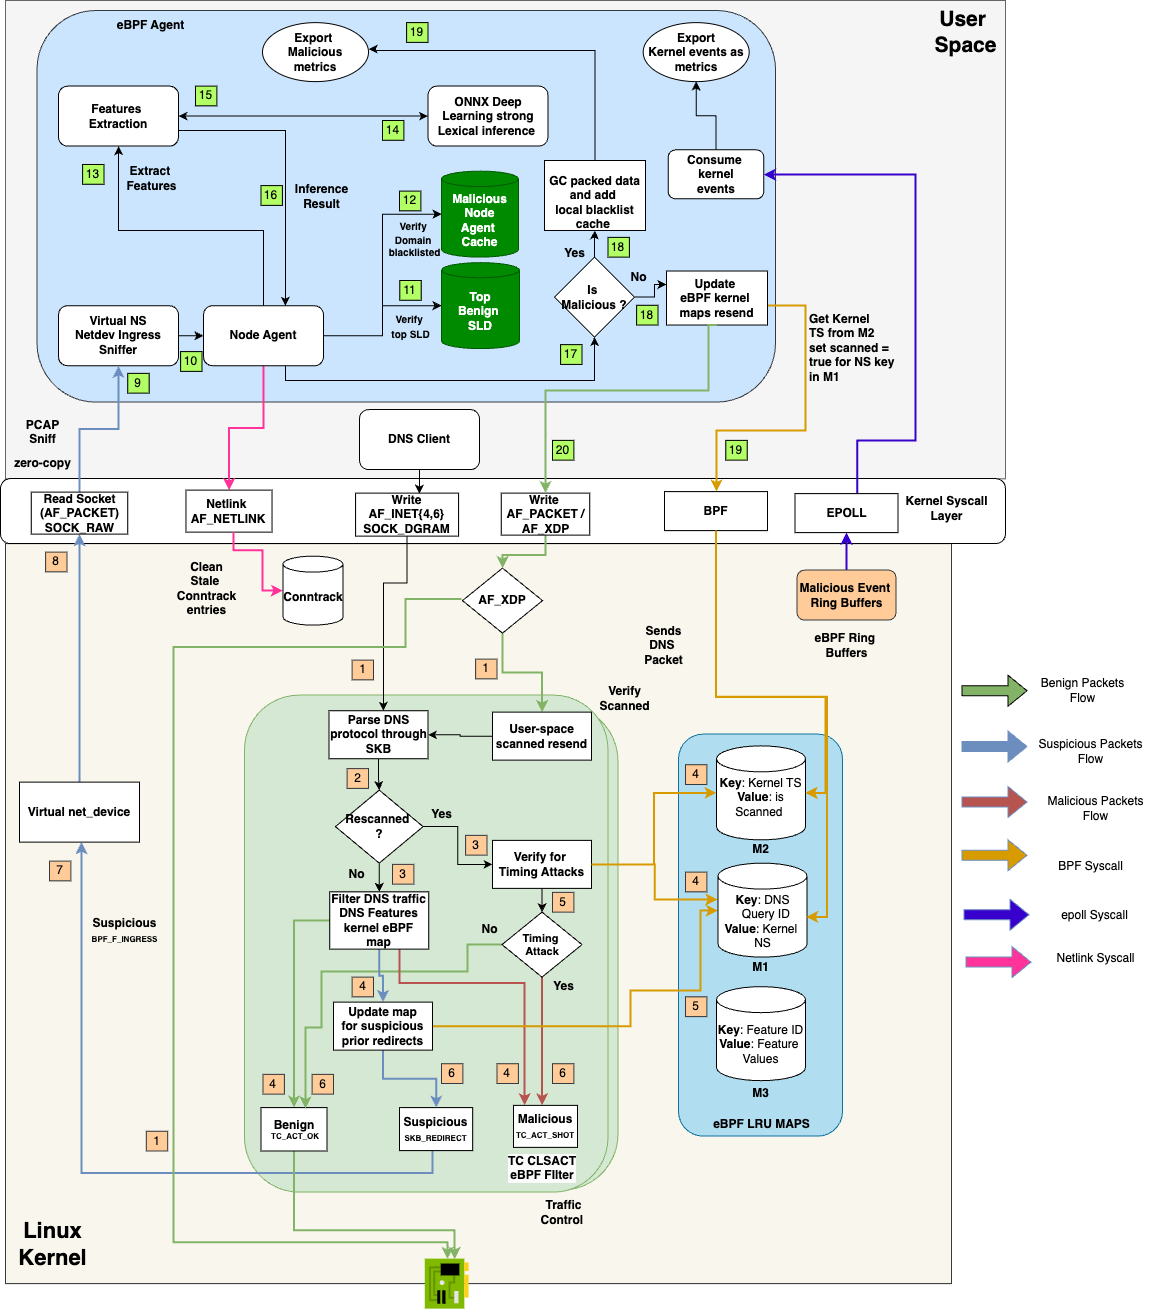
\includegraphics[width=1\textwidth]{UWThesis/images/udp-exfil-port-std.png}
\caption{eBPF Agent DNS Exfiltration Prevention Flow for Strict Enforcement Active Mode}
\label{sec:dp-active-phase}
\end{figure}

\subsection{Process-Aware Adaptive Passive Threat Hunting Mode}
\label{sec:passive}
The same eBPF program attached to the egress clsact TC filter, as described in \hyperref[sec:active]{active mode}, is reused for passive mode. It is attached to all physical netdev interfaces at the endpoint. The implementation of this mode is structured as follows: First, \hyperref[sec:maps]{maps} describes the eBPF map structures, their types, and their specific significance in passive mode. Second, \hyperref[passive:sec1]{kernel packet processing} details how the kernel eBPF program drops malicious exfiltrated packets, which are uniquely tied to the userspace processes responsible for sending them. This section also explains how additional kernel tracepoints, particularly those related to process scheduling, are used to perform garbage collection on map values. Third, \hyperref[passive:sec2]{userspace packet processing} outlines how the eBPF node agent handles packets in this mode. Finally, \hyperref[passive:sec3]{eBPF map concurrency} covers how the system maintains consistency between the kernel and userspace, even when multiple userspace threads and eBPF kernel programs scheduled in parallel across different CPU cores read or updates the eBPF maps.


% maps definition structure in passive phase 
\begin{figure}[H]
\centering
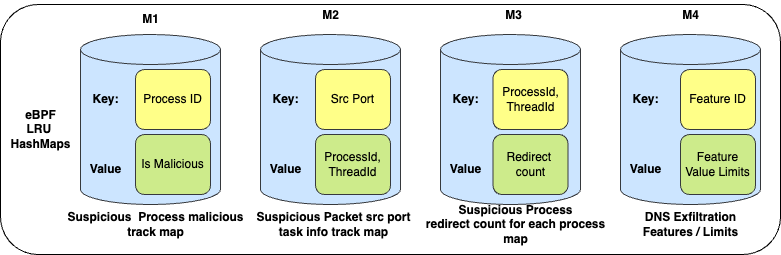
\includegraphics[width=1.0\textwidth]{UWThesis/images/map_struct_nport_53.png}
\caption{eBPF Maps and structure for Node agent in passive phase}
\label{sec:dp_eBPF_LRU_Maps_passive}
\end{figure}

\subsubsection{\textbf{eBPF Maps in Passive mode}}
\begin{enumerate}[itemsep=1pt,parsep=0pt]
\label{passive:maps}
\item \textbf{DNS Exfiltration Feature Map:} \\
Key: Feature identifier \\
Value: Filtering or classification parameter used by the eBPF TC egress program to process DNS traffic.

\item \textbf{Suspicious Process Redirect Count per process Map:} \\
Key: Process Info extracted from kernel task\_struct \\
Value: Count per process level suspicious redirected DNS layered over non-standard UDP DNS ports.

\item \textbf{Suspicious Packe:} \\
Key: Source Port of the potential layered DNS packet over random UDP port \\
Value: Process Info extracted from kernel task\_struct 


\item \textbf{Malicious Process Track Map}
Key: Process Info extracted from kernel task\_struct
Value: Is the Process malicioous based on previous detected malicious transfer through same process.
\end{enumerate}





\subsection{\textbf{eBPF program packet processing over egress TC QDISC filter}}
\label{passive:sec1}
In passive mode, DNS exfiltration is often attempted by layering DNS payloads over random UDP transport ports, excluding the standard DNS ports that are directly handled in active mode. The eBPF program parses the lower layers up to transports in the same manner as explained in active mode. As a deliberate design decision, these packets are not immediately redirected by the eBPF program, even if they appear suspicious. This prevents unnecessary network congestion and added latency for other legitimate Layer 7 protocols using arbitrary UDP ports. Since the eBPF program cannot guarantee that the application data in the skb truly belongs to DNS, it avoids aggressive redirection. Instead, it permits the packet to pass through the kernel as usual. Internally, however, it invokes \texttt{skb\_clone}, a kernel helper that creates a full clone of the packet from the original SKB.

In addition, because cloning packets increases memory usage, this mode avoids cloning all packets over random UDP ports. Instead, it attempts to raw-parse the SKB application data for potential DNS structures. If any validation exceeds the SKB limits (e.g., \texttt{skb->data\_end}), the packet is not considered DNS. If certain bounds align the SKB payload with potential DNS structures, additional checks are applied to validate that the application payload genuinely conforms to DNS, adhering to the limits defined in RFC 1035. \hyperref[sec:alg4]{Algorithm 4} explains these checks before performing clone redirection to the netdev owned by the eBPF node agent.

Prior to clone redirection, the eBPF TC program fetches the kernel \texttt{task\_struct} (process control block) via the \texttt{bpf\_get\_current\_pid\_tgid} helper, identifying the actual parent process and thread group ID in userspace involved in sending the packet. It then checks the \texttt{malicious\_process\_map} to determine whether the associated parent process ID has been flagged as malicious by userspace, based on previously detected DNS exfiltration attempts from the same process. If flagged, the eBPF program begins dropping the original packets but continues to clone and redirect them to userspace for monitoring. This behavior is referred to as a trap, where the kernel drops the packets yet keeps redirecting them to the eBPF node agent, allowing the agent to monitor the malicious implant’s retry behavior and gather runtime telemetry before taking termination action. This is an extremely robust and advance security design in the case of stealthy beaconing implants with randomized intervals. Once the implant’s parent process is flagged as malicious, subsequent beacon attempts are discarded in the kernel, forcing retries. The userspace agent observes these and collects system-level metrics to justify a kill signal against the offending process. Alternatively, if the process is not flagged as malicious, the eBPF program extracts the Layer 4 UDP port from the SKB and updates \texttt{src\_port\_task\_struct\_map} with the source port as the key and the extracted process ID and thread ID as the value. It also updates \texttt{task\_struct\_redirect\_ct\_map} with a composite key of process ID and thread ID, and an atomically incremented value representing the count of suspicious redirects. \hyperref[sec:alg5]{Algorithm 5} explains the eBPF map updates performed by the eBPF program in passive mode.
This continues until the process ceases sending DNS packets. If the process terminates and no malicious DNS activity was detected, cleanup is necessary to avoid dangling entries in \texttt{task\_struct\_redirect\_ct\_map}. For this purpose, an additional eBPF program is attached to the raw kernel tracepoint \texttt{tracepoint/sched/sched\_process\_exit}, which triggers when a process terminates or is killed. This tracepoint retrieves the exiting process’s information and removes its entries from both \texttt{task\_struct\_redirect\_ct\_map} and \texttt{malicious\_process\_map}.
The userspace eBPF node agent only sends a kill signal once the number of prevented DNS exfiltrations for a single process exceeds a configured threshold defined in the userspace agent’s configuration. If the process exits before reaching this threshold, the eBPF tracepoint program still ensures cleanup of \texttt{malicious\_process\_map} entries accordingly.

\subsubsection{\textbf{Userspace eBPF Node Agent Passive Mode}}
\label{passive:sec2}
The eBPF node agent launches concurrent, multiplexed goroutines—each pinned to a specific OS thread—to implement passive mode, which differs architecturally from active mode. These goroutines sniff traffic within a dedicated Linux namespace and its associated physical network device. They operate in zero-copy mode in userspace, similar to the active phase, where the kernel eBPF program redirects potentially layered DNS traffic for further inspection. All clone-redirected packets arriving in userspace contain both application data and lower-layer headers up to the transport layer. The userspace eBPF agent first parses the application payload, searching for embedded DNS structures. If no valid DNS layer is found, the extracted Layer 4 transport information is removed from the \texttt{src\_port\_task\_struct\_map}, using the source port as the key. If DNS data is identified within the tunneled application payload, the same evaluation logic as in active mode is followed. This includes extracting domain names and checking them against a local in-memory blacklist LRU cache. If a match is found, the domain is marked as blacklisted. Otherwise, the packet undergoes feature extraction and is passed to a deep learning model. If the model detects the packet as malicious, the userspace blacklist LRU cache is updated accordingly, and a detected threat event is streamed to the observability backend in the same manner as active mode. Since this is a clone-redirected packet, it is not re-injected into the network. Instead, the eBPF node agent uses the extracted source port to retrieve the associated process ID and thread ID from \texttt{task\_struct\_redirect\_ct\_map}, identifying a potentially malicious userspace process running alongside the eBPF node agent. After retrieving this information, the node agent updates the \texttt{malicious\_process\_map}, marking the parent process as malicious with a key-value entry of the process ID and a value of true. This allows the kernel eBPF program to drop all subsequent packets originating from that process. Additionally, the node agent examines rich telemetry from \texttt{task\_struct\_redirect\_ct\_map} — specifically, the number of times the packet was clone-redirected — using the process ID and thread ID as keys (retrieved via \texttt{src\_port\_task\_struct\_map}). If the redirected count exceeds a configurable threshold and the associated process has been flagged as malicious, the eBPF node agent — running with \texttt{CAP\_SYS\_ADMIN} capability — sends a kill signal to terminate the identified malicious process. With process-aware adaptive passive mode, the kernel eBPF program effectively aids the userspace agent in threat hunting processes that exfiltrate data over DNS via nonstandard UDP ports. Once identified, the eBPF agent terminates the malicious process in userspace. \hyperref[sec:alg6]{Algorithm 6} explains in detail how the eBPF node agent processes packets in passive mode.

\subsection{\textbf{eBPF Maps concurrency handling}}
\label{passive:sec3}
The map concurrency principles remain consistent with those in active mode, relying on per-CPU kernel spin locks with a globally shared eBPF map. This allows the eBPF program, scheduled across different CPUs, to update and reference-count map FDs, which remain alive as long as the eBPF node agent process is active in userspace. However, this mode introduces specific concurrency handling for map updates. For \texttt{src\_port\_task\_struct\_map}, the unique key—representing the source port—ensures atomic read and write operations, starting in the kernel when a DNS packet first arrives, followed by a corresponding read in userspace. Similarly, \texttt{malicious\_process\_map}, which is updated by the userspace eBPF node agent to mark processes as malicious, always uses the \texttt{BPF\_ANY} flag (create or update) for updates. As concurrent goroutines in userspace process sniffed packets in parallel, updates to this map are synchronized using a userspace mutex lock to ensure consistency. Since the kernel eBPF program across different CPUs only reads from this map, this design avoids blocking readers and improves packet processing throughput—similar to the RCU (read-copy-update) concept, which prioritizes performance and high-speed data access. Finally, for \texttt{task\_struct\_redirect\_ct\_map}, where the eBPF program in the kernel (executing on multiple CPUs) writes the redirect count while the eBPF node agent in userspace reads it, consistency is maintained using the eBPF map’s internal spin lock mechanism along with the \texttt{BPF\_ANY} update flag. Concurrent reads in userspace are synchronized via a separate userspace mutex, decoupled from the kernel’s per-CPU spin locks. The \hyperref[sec:dp-passive-phase]{Figure 4.5} details the full userspace and kernel pipeline over TC. 



% % alg 4
\begin{algorithm}[H]
\caption{DNS RAW SKB Parsing over Egress TC CLSACT QDISC in \textbf{Passive} Mode }
\label{sec:alg4}
\SetKwInOut{Input}{Input}
\SetKwInOut{Output}{Output}

\small % Reduce font size for the entire algorithm
\setstretch{0.9} % Reduce line spacing for more compactness

\Input{%
  \quad \texttt{skb} (socket buffer),\\
  eBPF LRU hash mapss:
  \quad \texttt{netlink\_links\_config}%
}
\Output{%
  \quad Packet Actions Clone Redirect action: \texttt{TC\_ACT\_OK} \\
  \quad eBPF Map Updates \texttt{bpf\_map\_updates}
}

Parse Lower layers from skb
% 
% Step 0: Extract DNS Header Counts
Parse DNS header from \texttt{skb}\;
% Step 1: Extract DNS Header Counts
Extract \texttt{qd\_count}, \texttt{ans\_count}, \texttt{auth\_count}, \texttt{add\_count}\;

% Step 2: Check for Non-Standard Port/Protocol
\tcp{Verify the DNS count limits within the header variable size (u8)}
\If{%
  \texttt{qd\_count} $\geq$ 256 \textbf{or} \\
  \quad \texttt{ans\_count} $\geq$ 256 \textbf{or} \\
  \quad \texttt{auth\_count} $\geq$ 256 \textbf{or} \\
  \quad \texttt{add\_count} $\geq$ 256%
}{
  \Return  \texttt{TC\_ACT\_OK}\;
}

% Step 3: DNS Flags and Opcode/Rcode Validation
Extract DNS flags: \texttt{raw\_dns\_flags} from \texttt{dns\_header}\;

\tcp{Verify the opcodes, rcode in DNS flag to validate RFC 1035}
\If{\texttt{opcode} $\geq$ 6}{
  \Return  \texttt{TC\_ACT\_OK}\;
}

\If{\texttt{rcode} $\geq$ 24}{
  \Return  \texttt{TC\_ACT\_OK}\;
}

% Step 4: Bridge Lookup and Redirection
Fetch \texttt{dst\_ip} and \texttt{bridge\_if\_index} from \texttt{netlink\_links\_config}:
\begin{itemize}[nosep]
    \item Key: \texttt{if\_index} (from \texttt{skb})
    \item Values: \texttt{dst\_ip}, \texttt{bridge\_if\_index}
\end{itemize}

Perform \texttt{bpf\_map\_updates}

\end{algorithm}


% % alg 5
\begin{algorithm}[H]
\caption{DNS eBPF map handling prior  in \textbf{PASSIVE} mode of agent}
\label{sec:alg5}
\SetKwInOut{Input}{Input}
\SetKwInOut{Output}{Output}

\small % Reduce font size for the entire algorithm
\setstretch{0.9} % Reduce line spacing for more compactness


\Input{%
  \texttt{skb} (socket buffer),\\
  eBPF LRU hash mapss: \\
  \quad \texttt{malicious\_process\_map},\\
  \quad \texttt{src\_port\_task\_struct\_map},\\
  \quad \texttt{task\_struct\_redirect\_ct\_map},\\
  \quad \texttt{dns\_packet\_clone\_redirection\_ct\_map}%
  \quad 
}

\Output{\texttt{bpf\_clone\_redirect} action to \texttt{bridge\_if\_index}}

% Step 1: Extract Transaction ID and Determine Network Layer
Parse DNS header from \texttt{skb}\;
Extract DNS transaction ID (\texttt{tx\_id}) from DNS header;

% Step 2: Fetch Virtualized Bridge Information
\tcp {if\_index resembles the netdev link index id in kernel}
Fetch \texttt{dst\_ip} and \texttt{bridge\_if\_index} from \texttt{netlink\_links\_config}:
\begin{itemize}[nosep]
    \item Key: \texttt{if\_index} (from \texttt{skb})
    % \item Values: \texttt{dst\_ip}, \texttt{bridge\_if\_index}
\end{itemize}
Fetch \texttt{skb\_mark} from \texttt{netlink\_links\_config}:
\begin{itemize}[nosep]
    \item Key: \texttt{if\_index}
    % \item Value: \texttt{skb\_mark}
\end{itemize}

Fetch process \texttt{task\_struct} and \texttt{process\_info} using \texttt{bpf\_get\_current\_pid\_tgid}:
\begin{itemize}[nosep]
    \item Key: \texttt{bpf\_get\_current\_pid\_tgid}
    % \item Value: \{\texttt{task\_struct}, \texttt{process\_info}\}
\end{itemize}

Fetch \texttt{is\_malicious} from \texttt{malicious\_process\_map} using \texttt{process\_id}:
\begin{itemize}[nosep]
    \item Key: \texttt{process\_id}
    % \item Value: \texttt{is\_malicious}
\end{itemize}

\If{not \texttt{is\_malicious}}{
    Update \texttt{src\_port\_task\_struct\_map} with:
        \begin{itemize}[nosep]
            \item Key:  \texttt{key=process\_id}
            \item Value: \texttt{value=task\_struct}
        \end{itemize}
    Fetch \texttt{current\_suspicious\_ct} from \texttt{task\_struct\_redirect\_ct\_map}:
    \begin{itemize}[nosep]
        \item Key: \texttt{task\_struct}
        % \item Value: \texttt{current\_suspicious\_ct}
    \end{itemize}
    Update \texttt{task\_struct\_redirect\_ct\_map} with:
    \begin{itemize}[nosep]
        \item Key: \texttt{task\_struct}
        \item Value: \texttt{current\_suspicious\_ct + 1}
    \end{itemize}
    Increment global \texttt{clone\_redirect\_ct} counter\;
    Update \texttt{dns\_packet\_clone\_redirection\_ct\_map} with:
    \begin{itemize}[nosep]
        \item Key: \texttt{if\_idx}
        \item Value: \texttt{new count}
    \end{itemize}
    Perform \texttt{bpf\_clone\_redirect(skb, bridge\_if\_index, BPF\_F\_INGRESS)}
}
\Else{
    Update \texttt{task\_struct\_redirect\_ct\_map} with:
    \begin{itemize}[nosep]
        \item Key: \texttt{task\_struct}
        \item Value: \texttt{current\_suspicious\_ct + 1}
    \end{itemize}
    \Return \texttt{TC\_ACT\_SHOT}\; \tcp{Drop the packet exfiltration attempt found over the process}
}
\end{algorithm}



% % alg 6
\begin{algorithm}[H]
\caption{User-Space eBPF Node Agent with Deep Learning and Event Streaming for DNS Traffic over Non-Standard UDP Ports}
\label{sec:alg6}
\SetKwInOut{Input}{Input}
\SetKwInOut{Output}{Output}

\small % Reduce font size for the entire algorithm
\setstretch{0.9} % Reduce line spacing for more compactness

\Input{Sniffed DNS packets from suspicious Linux namespaces via \texttt{pcap}; all kernel eBPF maps; eBPF LRU hash mapsss (\texttt{malicious\_process\_map}, \texttt{src\_port\_task\_struct\_map}, \texttt{task\_struct\_redirect\_ct\_map})}
\Output{Updates to \texttt{malicious\_process\_map}}

Sniff traffic over \texttt{veth} interfaces in isolated namespaces\;

\If{DNS layer \textbf{not} present in \texttt{skb\->data}}{
    \Return;
}

Extract L4 transport ports: \texttt{src\_port}, \texttt{dest\_port}\;
Extract DNS userspace features: \texttt{tx\_id}, \texttt{qd\_count}, \texttt{ans\_count}, query class/type, domain length\;

Fetch \texttt{task\_struct} from \texttt{src\_port\_task\_struct\_map} with:
    \begin{itemize}[nosep]
        \item Key: \texttt{src\_port} 
    \end{itemize}
% Extract \textit{process\_id} from \texttt{task\_struct} 

Extract \texttt{process\_id}, \texttt{thread\_group\_id} from \texttt{task\_struct}\;
% \texttt{malicious_process_map} with:
%     \begin{itemize}
%         \item Key: \texttt{process\_id}
%     \end{itemize}
Fetch \texttt{isBlacklistedSLDFound} from userspace LRU hash\;
\If{\texttt{isBlacklistedSLDFound}}{
    Update \texttt{is\_malicious flag} in \texttt{malicious\_process\_map} with:
    \begin{itemize}[nosep]
        \item Key: \texttt{kernel\_task\_struct}
        \item Value: \texttt{true}
    \end{itemize}
    Fetch \texttt{current\_suspicious\_ct} from \texttt{task\_struct\_redirect\_ct\_map} with:
    \begin{itemize}[nosep]
        \item Key: \texttt{task\_struct}
        % \item Value: \texttt{current\_suspicious\_ct + 1}
    \end{itemize}
    \If{\texttt{current\_suspicious\_ct} > \texttt{MAX\_MALICIOUS\_THRESHOLD}}{
        Send \texttt{SIGKILL} to \texttt{process\_id}\;
        \tcp {terminate the malicious process id extracted before from \texttt{src\_port\_task\_struct\_map}}
    }
    \Return;
}

Pass features to ONNX model for inference\;

\If{Inference == \texttt{MALICIOUS}}{
    Emit malicious threat events to message broker\;
    Blacklist SLD for related DNS records in userspace LRU malicious cache\;
    Update \texttt{is\_malicious flag} in \texttt{malicious\_process\_map} with:
    \begin{itemize}[nosep]
        \item Key: \texttt{kernel\_task\_struct}
        \item Value: \texttt{true}
    \end{itemize}
    Fetch \texttt{current\_suspicious\_ct} from \texttt{task\_struct\_redirect\_ct\_map} with:
    \begin{itemize}[nosep]
        \item Key: \texttt{task\_struct}
        % \item Value: \texttt{current\_suspicious\_ct + 1}
    \end{itemize}
    \If{\texttt{current\_suspicious\_ct} > \texttt{MAX\_MALICIOUS\_THRESHOLD}}{
        Send \texttt{SIGKILL} to \texttt{process\_id}\;
        \tcp {terminate the malicious process id extracted before from \texttt{src\_port\_task\_struct\_map}}
    }
    \Return;
}
\ElseIf{Inference == \texttt{BENIGN}}{
    \tcp*{No immediate action; future packets will be tracked and evaluated}
    \Return;
}
\end{algorithm}



\label{sec:data_plane_non_standard_port}
\begin{figure}[H]
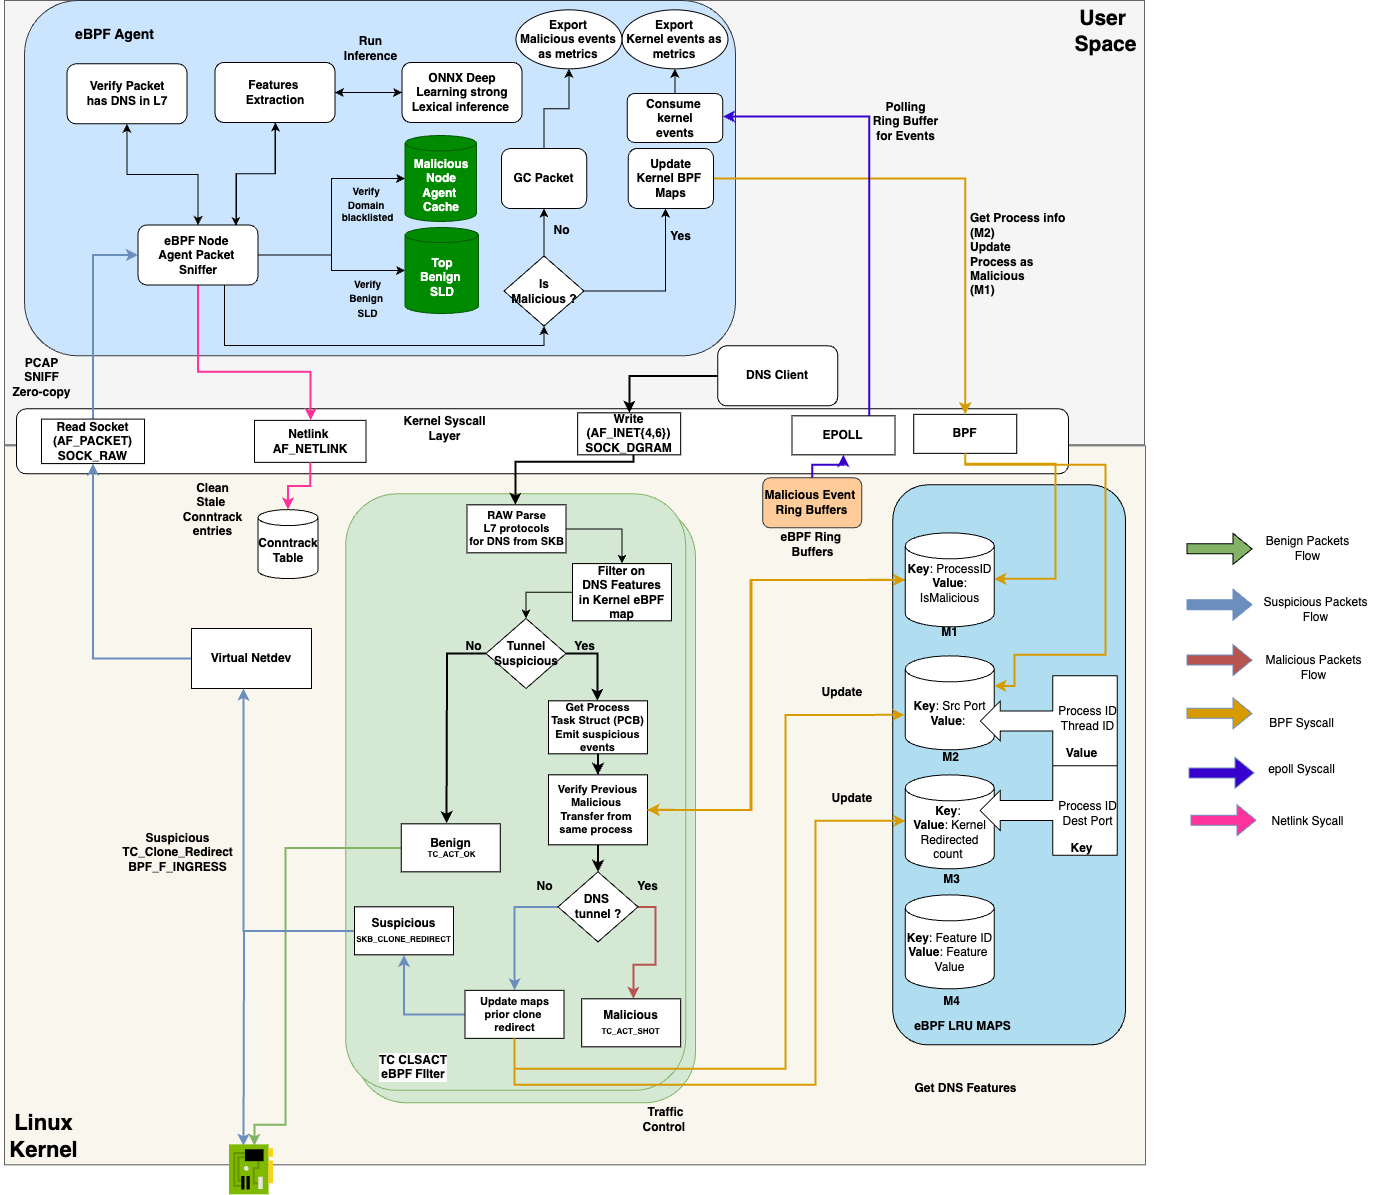
\includegraphics[width=1\textwidth]{UWThesis/images/udp-exfil-port-nstd.png}
\caption{eBPF Agent DNS Exfiltration Prevention Flow for Process-Aware Adaptive Mode of Agent}
\label{sec:dp-passive-phase}
\end{figure}


\subsection{DNS Exfiltration via Encapsulated Traffic}
In the Linux kernel network stack, encapsulated traffic is managed through virtualization drivers that extend the core \texttt{netdev} interface with associated RX and TX queues. These drivers support protocol encapsulation at various layers—L2, L3, and L4—by wrapping one protocol within another. 
The current implementation of the eBPF node agent focuses on L2-level encapsulation over software network devices, not on tunnels that rely on kernel cryptographic primitives via the keyring, such as those used by OpenVPN, IPsec, or WireGuard. This design choice aligns with the DNS protocol’s typical behavior, as DNS resolution rarely occurs over VPN tunnels. DNS exfiltration over encapsulated traffic in this context is limited to VLAN and TUN/TAP software network devices. VLAN encapsulation is similar and explained before in the SKB parsing in active phase by the TC eBPF program, where the eBPF program removes the L2 encapsulation layer (e.g., 802.1Q, 802.1AD) to expose the inner packet before proceeding with DPI.
TUN/TAP interfaces are virtual software devices exposed to userspace as file descriptors. Malicious userspace processes can write tunneled packets containing DNS data directly to these interfaces, bypassing standard inspection paths. The kernel handles L3 encapsulation at the sender side and performs L2 de-encapsulation on the TAP (receiver) side before forwarding traffic upstream. These devices, typically created using \texttt{iproute2} or \texttt{netlink}, forward traffic through a physical NIC. In its current state, the eBPF node agent handles only plaintext encapsulated traffic. Since encapsulation by these network drivers occurs at higher layers of the kernel network stack, the \texttt{skb} often lacks visibility into encapsulation details, except in the case of VLAN-tagged packets. To counter DNS tunneling over TUN/TAP interfaces, the agent injects \texttt{kprobes} on the \texttt{tun\_chr\_open} kernel driver function, which is responsible for creating tunnel interfaces. When a new TUN/TAP device is created, an event is pushed to userspace via a kernel ring buffer. The agent responds by attaching the same eBPF DPI program to the TC egress hook on the new interface, enforcing the same detection and prevention logic described in the active phase. 
Additionally, the exported ring buffer event includes rich telemetry about the process that created the tunnel, enhancing monitoring and threat attribution. \hyperref[sec:data_plane_tunnel_netdev]{Figure 4.6} illustrates the detailed flow.



\begin{figure}[H]
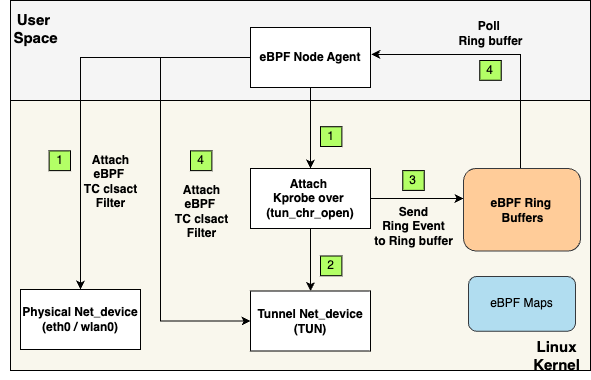
\includegraphics[width=1\textwidth]{UWThesis/images/udp-exfil-tunnel-netdev-tun_tap.png}
\caption{eBPF Agent Prevention flow over Tun/Tap Driver kernel function}
\label{sec:data_plane_tunnel_netdev}
\end{figure}



\subsection{Feature Analysis in Data Plane}
\label{sec:features}
The eBPF node agent filters traffic directly in kernel space using statically populated values in eBPF maps. These values modify packet processing and scheduling logic by correlating DNS packet fields within the kernel’s socket buffer (sk\_buff) with predefined threshold limits. The kernel’s traffic control (TC) subsystem enforces this logic at runtime, inspecting and filtering each packet as detailed in the ingress and egress processing sections.

DNS packets over UDP are restricted to 512 bytes of data, regardless of the MTU (Maximum Transfer Unit) of the network interface. According to RFC 1035, DNS domains have a maximum length of 255 characters (including periods) and must adhere to specific label length limits (127 characters maximum per label and 63 characters per individual label) for queries such as A (address) records. Other query types like TXT and NULL may contain non-domain information, yet still remain within the 512-byte UDP limit. For larger payloads, the EDNS extension allows fragmentation, while TCP-based DNS transport also supports larger payloads without exceeding these limits.

The implementation is divided into two parts. First, the  \hyperref[sec:kernel-features]{kernel features} used by eBPF programs are explained, focusing on classifying, filtering and redirecting suspicious DNS packets. Second, the features used by the userspace deep learning model for enhanced lexical analysis of DNS payloads to detect obfuscation in exfiltrated packets are discussed.
\subsubsection{Kernel-space features}
\label{sec:kernel-features}
Due to kernel-level restrictions imposed by the eBPF verifier, DPI is limited to the first DNS question record, parsed from the DNS header by the eBPF TC program attached in the egress path. This design aligns with modern DNS behavior, as legitimate queries almost always contain a single question; thus, detection of multiple questions (via the qd\_count field) is treated as a strong anomaly signal. Feature selection was guided by common patterns in DNS tunneling and C2 abuse while ensuring in-kernel efficiency. Numeric features such as domain length and label count are compared against minimum and maximum thresholds configured by the userspace loader during initialization. Suspicious DNS query types like NULL and TXT are flagged due to their ability to carry arbitrary payloads, while any query class other than “Internet” (IN), per RFC 1035, is also considered anomalous. These features are inserted into a kernel feature map for real-time classification. If a feature exceeds its threshold, it is marked malicious; if within bounds, it is flagged suspicious; otherwise, it is benign. This classification logic is uniformly applied across both active and passive modes, even for encapsulated traffic, where tunnel headers are removed before inspection. The features were chosen for semantic relevance to DNS abuse, verifier safety, and low overhead, enabling fast, accurate classification and real-time enforcement entirely within the kernel. The kernel features are detailed in \hyperref[sec:feature-kernel]{Table 4.3}.

\subsubsection{Userspace deep learning model features}
\label{sec:userspace-features}
The deep learning model is trained on eight lexical features detailed in \hyperref{sec:feature-userspace}{userspace features}. These features were selected through an in-depth analysis of DNS exfiltration behavior, based on real-world attack samples, open-source C2 toolkits, and proprietary DNS tunneling frameworks. The focus is on detecting encoded payloads embedded in DNS queries by analyzing structural and statistical anomalies in the query format. Specifically, malicious queries often exhibit either an unusually high number of labels (subdomains) or fewer labels with unusually long lengths, both exploiting the limits of RFC 1035: 63 characters per label, 127 total labels and 255 characters overall. Moreover, encoding algorithms as explained before often introduces high entropy and randomness in the payload. These characteristics, derived from protocol-aware inspection and empirical adversary behavior, form the input to the model. Table \hyperref{sec:feature-userspace}{Table 4.4} summarizes the complete set of features.


\subsection{Datasets}
\label{sec:dataset}
The trained deep learning model utilizes three main datasets for training. First, Cisco’s top 1 million SLDs are not used for model training, but instead are loaded into an in-memory LRU cache by the eBPF node agent as the most benign SLD. This design optimizes performance by preventing model inference on these domains, since any sniffed DNS traffic containing them in the SLD will not be an exfiltrated packet because their auth zones are owned by authorized sources. Note that as explained before, reliance on domain scoring is used, however, the LRU cache is completely reprogrammable from the control plane. Second, for model training, it uses the DNS exfiltration dataset by \citeauthor{ziza2023dns}, which includes live-sniffed DNS traffic from an ISP, consisting of around 50 million benign and malicious samples \cite{ziza2023dns}. Due to the smaller number of malicious samples compared to benign ones, and to avoid training bias, a synthetic dataset was generated using open-source exfiltration tools—DET, DNSExfiltrator, DNSCat2, Sliver, Iodine and custom DNS exfiltration scripts. These exfiltrated datasets captured all forms of data obfuscation for different encoding or encryption algorithms as explained  \hyperref[dns_payload_obfuscation]{before} , including tunneling and raw exfiltration, across a wide range of file formats including text (markdown, txt, rst, raw config files), image (jpg, jpeg, png), and video (mp4), generating a combined dataset of around 6 million domains, covering all the exfiltration patterns , with 50\% benign and the remaining malicious.


% % feature table 1 Kernel
\begin{table}[ht]
\centering
\resizebox{\textwidth}{!}{
\begin{tabular}{|c|l|}
\hline
\textbf{Feature} & \textbf{Description} \\
\hline
\texttt{subdomain\_length\_per\_label} & Length of the subdomain per DNS label. \\
\texttt{number\_of\_periods} & Number of dots (periods) in the hostname. \\
\texttt{total\_length} & Total length of the domain, including periods/dots. \\
\texttt{total\_labels} & Total number of labels in the domain. \\
\texttt{query\_class} & DNS question class (e.g., IN). \\
\texttt{query\_type} & DNS question type (e.g., A, AAAA, TXT). \\
\hline
\end{tabular}
}
\caption{DNS Features in Kernel}
\label{sec:feature-kernel}
\end{table}


% feature table 2 userspace
\begin{table}[ht]
\centering
\resizebox{\textwidth}{!}{
\begin{tabular}{|c|l|}
\hline
\textbf{Feature} & \textbf{Description} \\
\hline
\texttt{total\_dots} & Total number of dots (periods) in the \texttt{request} (domain name). \\
\texttt{total\_chars} & Total number of characters in the \texttt{request}, excluding periods. \\
\texttt{total\_chars\_subdomain} & Number of characters in the subdomain portion only. \\
\texttt{number} & Count of numeric digits in the \texttt{request}. \\
\texttt{upper} & Count of uppercase letters in the \texttt{request}. \\
\texttt{max\_label\_length} & Maximum label (segment) length in the \texttt{request}. \\
\texttt{labels\_average} & Average label length across the \texttt{request}. \\
\texttt{entropy} & Shannon entropy of the \texttt{request}, indicating randomness. \\
\hline
\end{tabular}
}
\caption{DNS Features in Userspace}
\label{sec:feature-userspace}
\end{table}


\subsection{Deep Learning Model Architecture}
\label{sec:ml}
The deep learning architecture in userspace enhances the eBPF node agent’s detection accuracy across a broad spectrum of obfuscation techniques within DNS payloads—capabilities that are otherwise infeasible to implement directly within kernel space due to eBPF verifier constraints. The model employs a sequential dense neural network architecture  built using TensorFlow over the dataset generated and labelled as explained before, taking 8 lexical input features that aid detection in identifying exfiltrated DNS obfuscation patterns. The input during model training is handled using TensorFlow shufflers with a configured batch size. The pipeline shuffles the data and prefetches data using tensorflow autotune policies for efficient prefetching of data batches minimize I/O for large dataset of around 6 millions rows. Moreover, the model relies on distributed mirrored strategy of tensorflow for efficient parallel usecase of GPU resources.
It consists of three hidden dense layers, each with 16 neurons, and a final output layer with a single neuron for binary classification. ReLU (Rectified Linear Unit) is used as the activation function between layers, while the output layer uses sigmoid activation due to the binary nature of the final output layer. The model is compiled using the Adam optimizer with fine tuned finalized learning rate of 0.001 ensure stable and efficient convergence during training. The binary cross-entropy loss function is used specifically due to binary classification requirement for detecting a specific feature extracted from DNS payload as bengin or malicious. Total of 25 epochs were selected to optimize model weights ensuring enough compared to dataset size to prevent the model from overfitting. 
Once trained, the model is exported to the ONNX (Open Neural Network Exchange) graph format for use in live inference on kernel-redirected or clone-redirected suspicious traffic. To minimize memory footprint and improve inference speed, the model is integrated into the eBPF userspace agent as a submodule via the ONNX Runtime. Communication between the ONNX-loaded submodule and the core eBPF agent is handled through Unix domain sockets (IPC). Although this design introduces some inference latency, it is mitigated by a first-line caching layer that includes an LRU-based blacklist and a top-level SLD domain cache within the core eBPF agent process, improving efficiency for repeated inferences on identical inputs. This architecture was chosen due to the limited maturity of ONNX ecosystem support in Go.
The ONNX-based inference submodule of the eBPF node agent also supports optional hardware acceleration on CPU or GPU when available at the endpoint. To further optimize runtime efficiency, the model is loaded after undergoing dynamic quantization using ONNX’s quantizer, which internally applies per-neuron dynamic quantizers and casters to convert float32 vectors into lower-precision formats. This significantly reduces memory usage and computational overhead. Compared to formats such as HDF5 or Pickle, ONNX provides a lightweight, runtime-efficient graph representation, enabling fast, low-overhead inferencing and ensuring the agent maintains a minimal memory footprint even under peak load conditions. \hyperref[sec:model_arch]{Figure 4.7} illustrates the deep learning quantized model architecture as internally represented in ONNX graph. 




\begin{figure}[H]
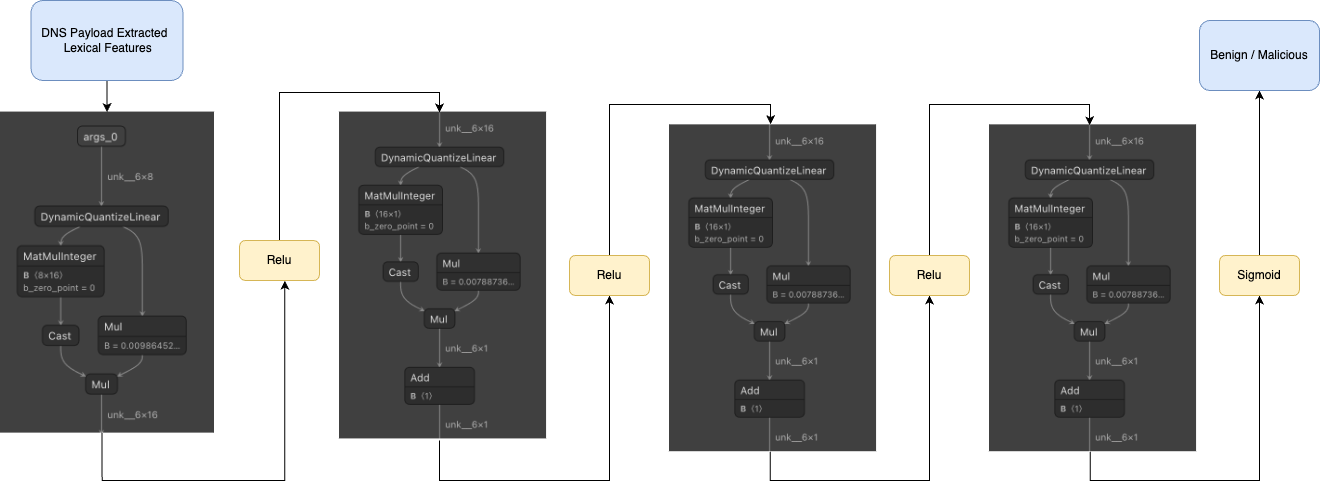
\includegraphics[width=1\textwidth]{UWThesis/images/DNN_Model_Arch.png}
\caption{DNS Data obfuscation detection Deep Learning Model Architecture}
\label{sec:model_arch}
\end{figure}





% The eBPF node-agent running in userspace at the endpoint in privileged context interacts with kernel network stack over the kernel TC layer leveraging eBPF as a classless leaf QDISC to behave both as a classifier for TC in kernel subsysttem as well as a  used for egress packet scheduling to the network device driver by injecting eBPF programs behaving as filters encapsulating logic for DPI, In addition to  core kernel network datapath these agents also inject programs over kernel LSM (Linux Security Modules), syscall for raw tracepoints for secured access control and injection and verification of the integrity of eBPF programs in kernel via kernel keyring and cert verification, gathering metrics related to process scheduling and finally kernel syscall layer to terminate the malicious implant process, once exceed threshold of being detected and prevented carrying data exfiltration of C2 channels over DNS and finally eBPF raw kernel probes over netdev device driver functions to trigger events from kernel emitted via eBPF ring buffer polled by agent in userspace to dynamically inject kernel security eBPF programs over these virtual net devices to prevent any form of encapsulated exfiltration  The entire implementation is  divided two main root categories first describing the flow how agent operates and prevents DNS exfiltration  for non-encapsulated network traffic often done via physical network devices at the endpoint, followed with breach prevention for encapsulated traffic via virtual network interfaces. Implementation for each type describes how the agent prevents data exfiltration over DNS over egress direction of kernel network datapath, eBPF programs implementation within kernel TC, ebpf map handling, and finally userspace agent tasks including deep learning model inference for deep scanning suspicious traffic and resending packets via high speed kernel datapath and addon eBPF validation post resend to reduce attack vectors for timing and brute-force attacks, in both phases of operation active and passive modes. The term DNS data exfiltration refers to all forms of exfiltration packets send irrespective of techniques in userspace (DNS C2, DNS tunneling, DNS raw exfiltration). The eBPF program over kernel TC faciliate both mode of operation active / passive based on how the userspace agent loader injects the program configured via agent loader config. The userspace behav For both both of operations active and passive, single kernel TC programs faciliate 











% \subsection{Active Phase}
% Post injection of single eBPF TC CLSACT QDISC filter with highest priority attached to all the physical network devices at the endpoint in egress direction as a leaf filter in the hierarchical structure kernel TC if the network devices are using classful filters or classless filters, to intercept every single packet flowing over egress direction at the endpoint. In active mode, the primary goal for the TC QDISC filter is to parse the DNS layer in sk\_buff for enhanced intelligence to detect exfiltrated DNS packets and drop, redirect, forward the packets upstream. The eBPF programs utilizing default kernel CLSACT QDISC action post classification of DNS packets using TC\_ACT\_SHOT for dropping the packet, TC\_ACT\_OK to forward packet, and SKB kernel function helper SKB\_redirect to redirect the packet to rx quesues of  different netdev at the endpoint.







%  Trafic without encapsulation (i.e., not using virtual interfaces or overlay networks) have a single header and payload, with protocol layers determined by the transfer protocol. Based on the structure of such packets, the DPI is fundamentally divided into two main scenarios based on different Layer 3 (network) and Layer 4 (transport) protocols. Since DNS being and Layer 7 or Application layer protocol, for a packet to have \ac{dns} in its application data, it requires the packet to either have \texttt{ETH\_P\_IPV4} (IPv4) or \texttt{ETH\_P\_IPV6} (IPv6) as the network layer, and \texttt{IPPROTO\_UDP} (UDP) or \texttt{IPPROTO\_TCP} (TCP) as Layer 4 for transport. Because the agent at the endpoint only considers potential DNS exfiltration prevention over UDP, if DNS packet over TCP is found it is allowed to passthrough assuming traffic filtering would be done over DNS server as explained before. Hence only considering DNS traffic over UDP, the DPI  is performed in the following manner to extract the \ac{dns} layer in raw bytes present in the SKB. The forwarding decision in the filtering is based on the mode of operation the agent in userspace decided to inject these programs which would be explained in depth in consecutive sections. The next sections explains complete end to end flow how DNS exfiltrated packets are prevented from kernel eBPF programs and userspace over egress and ingress directions of network datapath for both active and passive modes.


% Active Mode:
% If the agent is running at the endpoint in an active mode, the primary goal is to prevent almost no exfiltrated packets to passthrough over default ports used for DNS as per RFC 1035. 
 
 
 
 
%  While the security framework also performs DPI over raw socket buffers with transport via non-standard DNS ports to prevent packet tunneling of DNS payloads over other ephemeral ports used by different protocols, the following explains the different scenarios over which \ac{dpi} is performed. It further details the filtering algorithm used in the eBPF traffic control direct-action filter to either drop, forward, or redirect the egress packet to a different interface for further \ac{dpi}.











% % \ElseIf{Namespace handles clone redirected DNS traffic (non-standard ports)}{
% %     Fetch \texttt{val = \{dst\_port, src\_port, isUdp, isPacketRescannedAndMalicious\}} 
% %     from \texttt{dns\_clone\_redirect\_map}\;
% %     \If{Packet contains DNS layer}{
% %         Blacklist SLD for all DNS queries\;
% %         \textbf{return};
% %     }
% %     \Else{
% %         Set \texttt{val.isPacketRescannedAndMalicious = true}\;
% %         Update \texttt{dns\_clone\_redirect\_map}[\texttt{dst\_port}] = \texttt{val}\;
% %     }
% % }

\begin{table}[ht]
\small
\newcolumntype{L}[1]{>{\raggedright\arraybackslash}p{#1}}
\centering
\begin{tabular}{|L{5cm}|L{10cm}|}
\hline
\textbf{Kafka Topic Name} & \textbf{Description} \\
\hline
\texttt{exfil-sec} & Kafka topic used by the node agents in data plane to stream prevented DNS threat events. \\
\hline
\texttt{exfil-sec-infer-controller} & Topic used by the controller to publish dynamic domain blacklists to DNS servers for data plane eBPF agent update userspace caches. \\
\hline
\end{tabular}
\caption{Kafka Stream Topics Used in the eBPF Node Agent}
\label{tab:kafka-topics}
\normalsize
\end{table}



% \label{sec:data_plane_ingress_sniff}
% \begin{figure}[h]
% 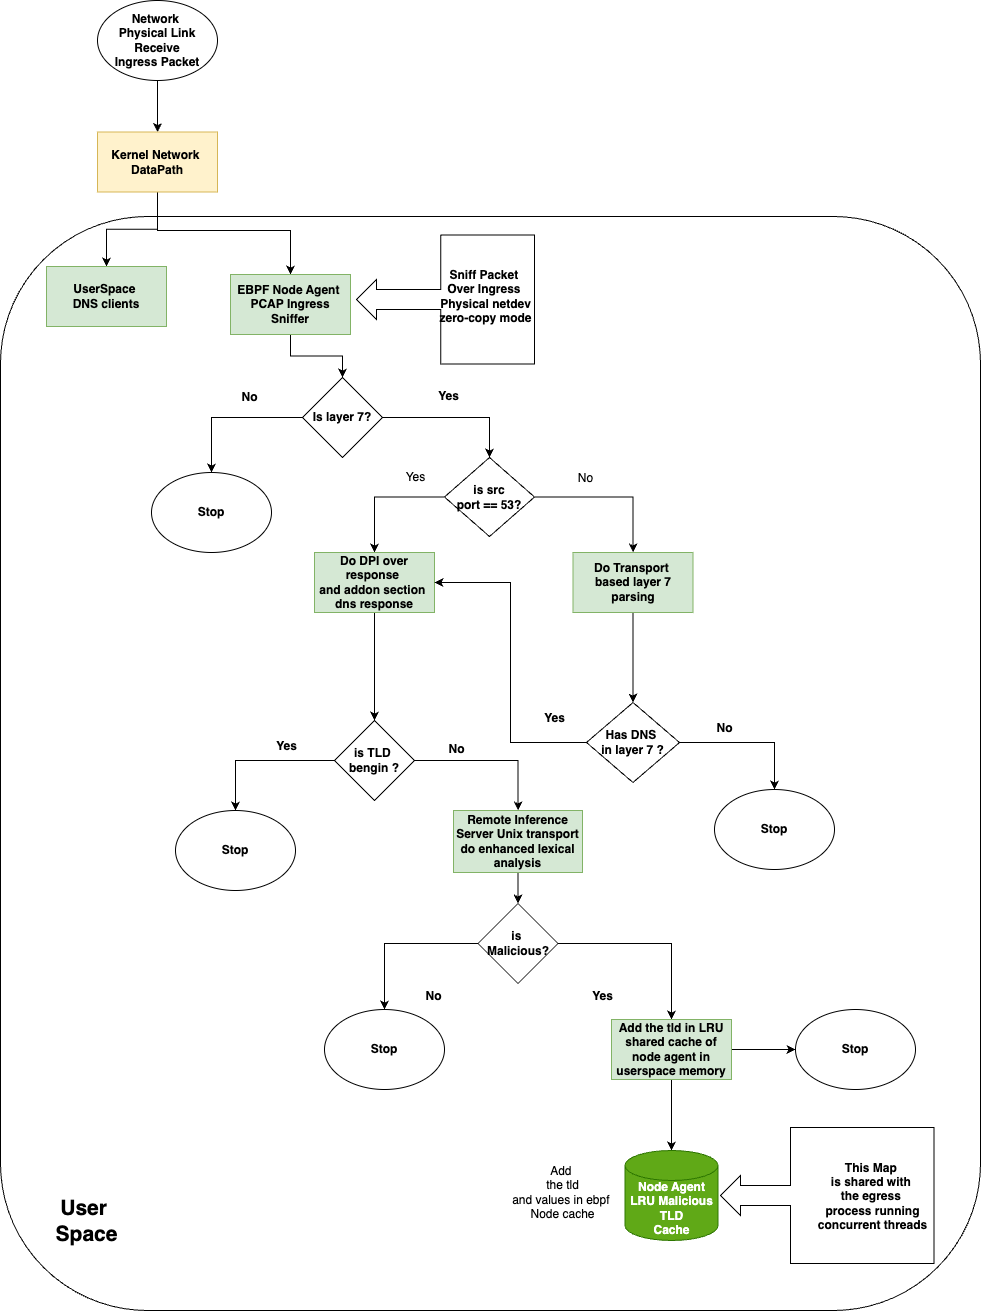
\includegraphics[width=1\textwidth]{UWThesis/images/udp-exfil-ingress-sniff-flow.png}
% \caption{eBPF Agent DNS Exfiltration Prevention Flow ingress DNS traffic analysis}
% \end{figure}


\subsection{Thread Events Streaming and Metrics Exporters}
The eBPF node agent in the data plane operates in both active and passive modes. When a DNS packet is flagged as malicious and contains an exfiltrated payload, the agent streams a threat event using Kafka producers. These producers are embedded in the compiled eBPF userspace binary and are configured to send data to a remote Kafka broker. Each eBPF node agent also includes Kafka consumers. Every agent is assigned a unique application ID derived from the local node’s IP address, combined with a randomly generated ID to form the Kafka consumer group ID. This design ensures strong decoupling between agents, enabling massive horizontal scalability—data plane nodes can scale independently without relying on a shared consumer group. Kafka producers operate asynchronously, allowing the agent to emit threat events while concurrently consuming control plane topics streamed by the inference controller. These topics carry resolved malicious domains, enabling each data plane node to update its local blacklist even if the exfiltration was detected on a different node. This improves prevention accuracy across the cluster. Additionally, consumed events allow eBPF node agents to apply dynamic Layer 3 filters in the kernel, supporting cross-protocol correlation. While threat events focus on detected exfiltration attempts, the kernel-space eBPF programs also export deep system-level metrics. These metrics are exposed via Prometheus, allowing the controller to scrape and monitor them across all nodes in real time. This centralized observability supports both the analysis of blocked threats and continuous system behavior tracking.   \hyperref[tab:kafka-topics]{Table 4.5} explains the details.
% For details, see \hyperref[sec:dp_ebpf_node_metrics]{eBPF node metrics}.

\section{Control Plane}
As illustrated in the control plane component overview, the controller is designed to be entirely stateless, relying on the GPSQL backend used by PowerDNS for DNS state management and RPZ zones for tracking malicious domains. The control plane currently consists of a single Tomcat web server, with Spring Kafka consumer integrated to consume malicious threat events from the exfil-sec Kafka topic. These events are emitted by all endpoints in the data plane and contain metadata of blacklisted domains and node-level context identifying where the threat was detected. Upon consuming these events, the control plane dynamically updates the RPZ backend with the (SLDs) associated with malicious domains in threat events. This update enforces DNS-level security enforcement making the DNS server start dropping any queries to these domains. To optimize performance and prevent malicious DNS queries from ever reaching the DNS server again once blacklisted, the control plane also writes to another Kafka topic (exfil-sec-infer-controller). This topic is consumed by all data plane nodes to rehydrate their local malicious userspace caches, effectively reprogramming the eBPF node agents at each endpoint to drop related packets immediately at the endpoint reducing network hops. For enhanced security, the control plane additionally performs DNS resolution on the malicious domains to extract their corresponding layer 3 addresses. These addresses, which  represent active C2 or tunneling servers on the public internet, are also streamed in exfil-sec-infer-controller Kafka topic used to dynamically enforce layer 3 network policies inside the kernel post consumed by the eBPF agents deployed across the data plane for cross protocol coorelation. With fully asynchronous, bidirectional communication between the control plane and data plane via Kafka, the architecture enables continuous reprogrammability of data plane nodes to enforce dynamic, kernel-level security policies. It also supports horizontal scalability of individual components crucial for production-grade cloud environments. This design directly targets and stops DGAs, providing robust protection against mutation at both Layer 3 (IP addresses) and Layer 7 (domain names).


\section{Distributed Infrastructure }
As explained earlier in the security framework overview, the distributed infrastructure primarily consists of a PowerDNS authoritative DNS server, a PowerDNS recursor, a generic GPSQL backend (PostgreSQL), Kafka brokers, and Prometheus metric scrapers. These scrapers collect metrics exposed by the eBPF node agents deployed in the data plane. The eBPF agents do not handle malicious DNS exfiltration over TCP due to the inherent complexity of the TCP state machine within the kernel, once packets have passed through Netfilter in both ingress and egress paths of the TCP/IP network stack. To address this gap, TCP-based DNS exfiltration attempts are intercepted in userspace by PowerDNS recursor query interceptors, as a middleware with \hyperref[sec:alg7]{Algorithm 7} explains the details. As the PowerDNS recursor currently only supports Lua-based interceptors, a custom Lua interceptor was developed to process DNS queries received over TCP from data plane nodes. This interceptor extracts features from the query and performs inference using a serialized ONNX-based deep learning model. Leveraging Lua’s lightweight and high-performance characteristics, the recursor also accesses the GPSQL backend, which contains an additional table maintained by the controller. As previously discussed, this table serves as an RPZ (Response Policy Zone), enabling efficient \texttt{NXDOMAIN} responses for queries involving known malicious domains. Before triggering inference, the Lua interceptor checks whether the domain is already blacklisted, allowing it to skip inference for improved throughput. To further enhance performance, the interceptor uses PowerDNS internal Domainsets—a fast, in-memory trie-based data structure—for caching malicious domains detected over TCP. This enables rapid filtering of repeated exfiltration attempts. Additionally, the Lua interceptor periodically synchronizes with the RPZ, rehydrating the local Domainset cache to ensure up-to-date enforcement without incurring inference overhead.

% alg 7
\begin{algorithm}[H]
\caption{\texttt{PowerDNS DNS Query Interceptor}}
\label{sec:alg7}
$qname \gets dq.qname.toString()$\;

\small % Reduce font size for the entire algorithm
\setstretch{0.9} % Reduce line spacing for more compactness

\If{$dq.isTcp$}{
    $result \gets \text{extractFeaturesAndGetremoteInference}(qname)$\;
    \If{$\text{result}[\texttt{"threat\_type"}]$}{
        insertMaliciousDomains($qname$)\;
        $dq.rcode \gets \texttt{NXDOMAIN}$\;
        \Return \textbf{true}\;
    }
}
\If{$sf\_blacklist.\text{check}(\text{getSLD}(qname))$}{
    $dq.rcode \gets \texttt{NXDOMAIN}$\;
    \Return \textbf{true}\;
}
\If{$sf\_blacklist.\text{check}(\text{getSLD}(qname))$}{
    $dq.rcode \gets \texttt{NXDOMAIN}$\;
    \Return \textbf{true}\;
}
\Return \textbf{false}\;
\end{algorithm}


% \label{sec:data_plane_overview_deep}
% \begin{figure}[H]
% 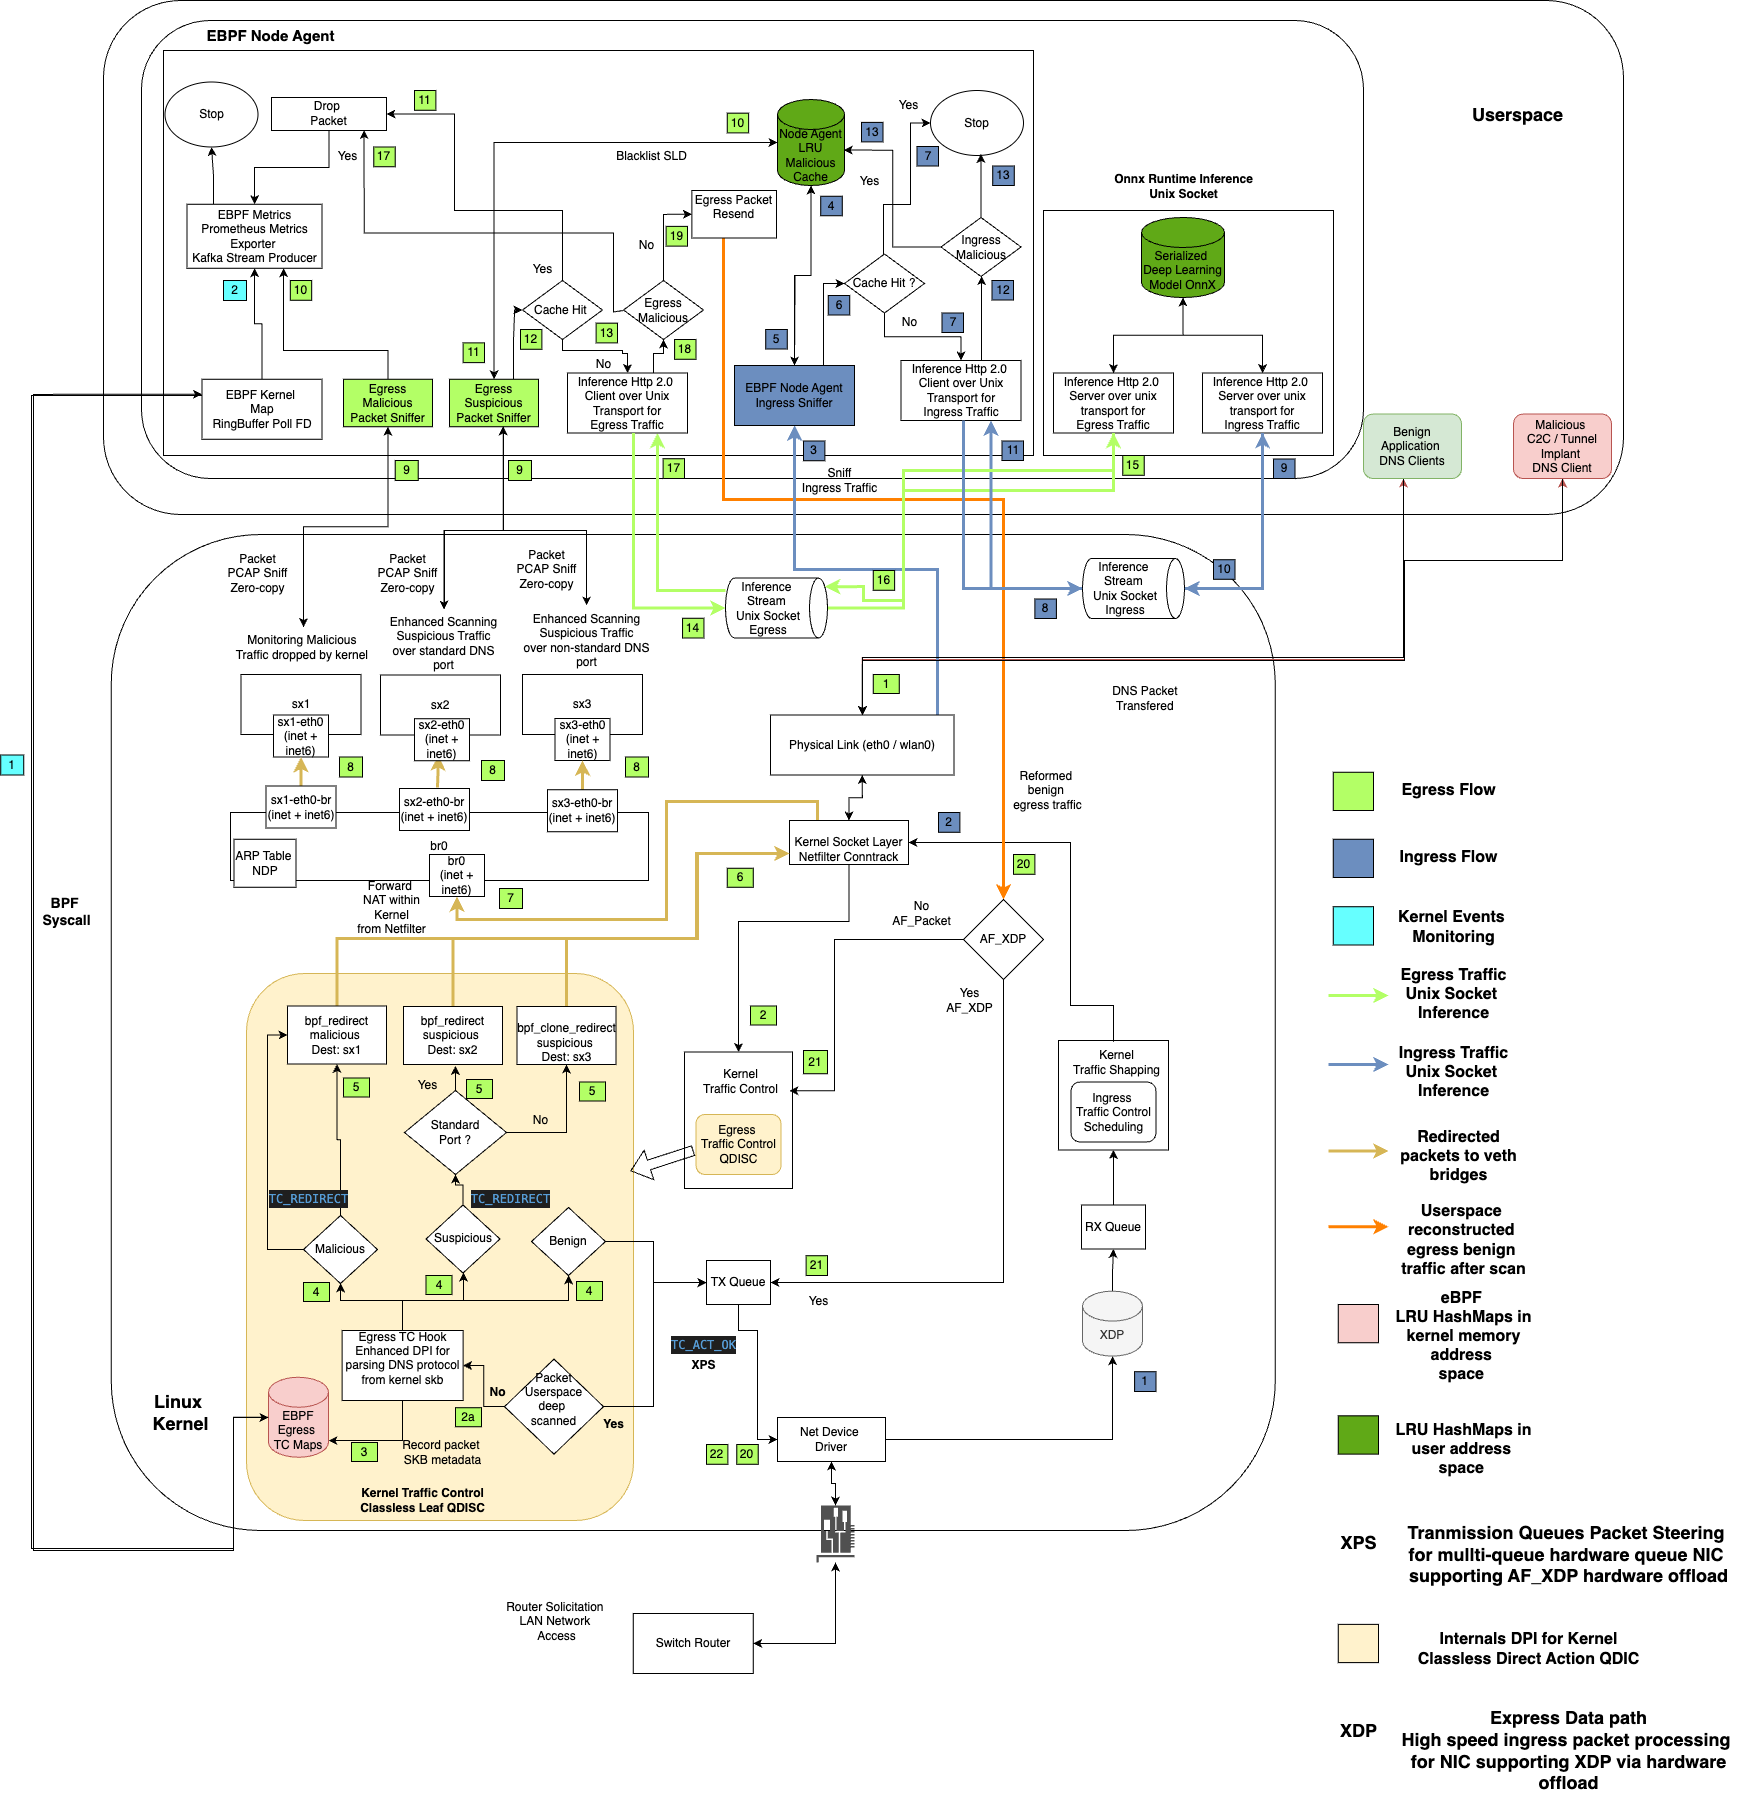
\includegraphics[width=1\textwidth]{UWThesis/images/dataplane_deep.png}
% \caption{Data Plane eBPF Agent Complete flow}
% \end{figure}





\chapter{Evaluation}
This chapter evaluates the effectiveness of the security framework in a distributed setting with  comprehensive evaluation results and analysis.


\section{Environment Setup}
The security framework was deployed across CSSVLAB{01–08} nodes running over Ubuntu 24.02 on Linux kernel 6.12 on Intel(R) Xeon(R) Gold 6130 (x86\_64) architecture, each with 8 GB of memory and 24 GB of storage. The test bench launches a custom PowerDNS authoritative and recursor server on CSSVLAB08. The controller and a Kafka single-broker instance run on CSSVLAB01. Nodes CSSVLAB{02–07}, excluding CSSVLAB06, act as the data plane, each running the eBPF node agent and using the custom PowerDNS server as the default resolver via systemd-resolved. CSSVLAB06 is used to simulate DNS exfiltration attacks against data plane nodes, tunneling DNS queries through the same PowerDNS instance. The full deployment is illustrated in \hyperref[sec:deployed-arch]{Figure 5.1}.


\begin{figure}[h]
\centering
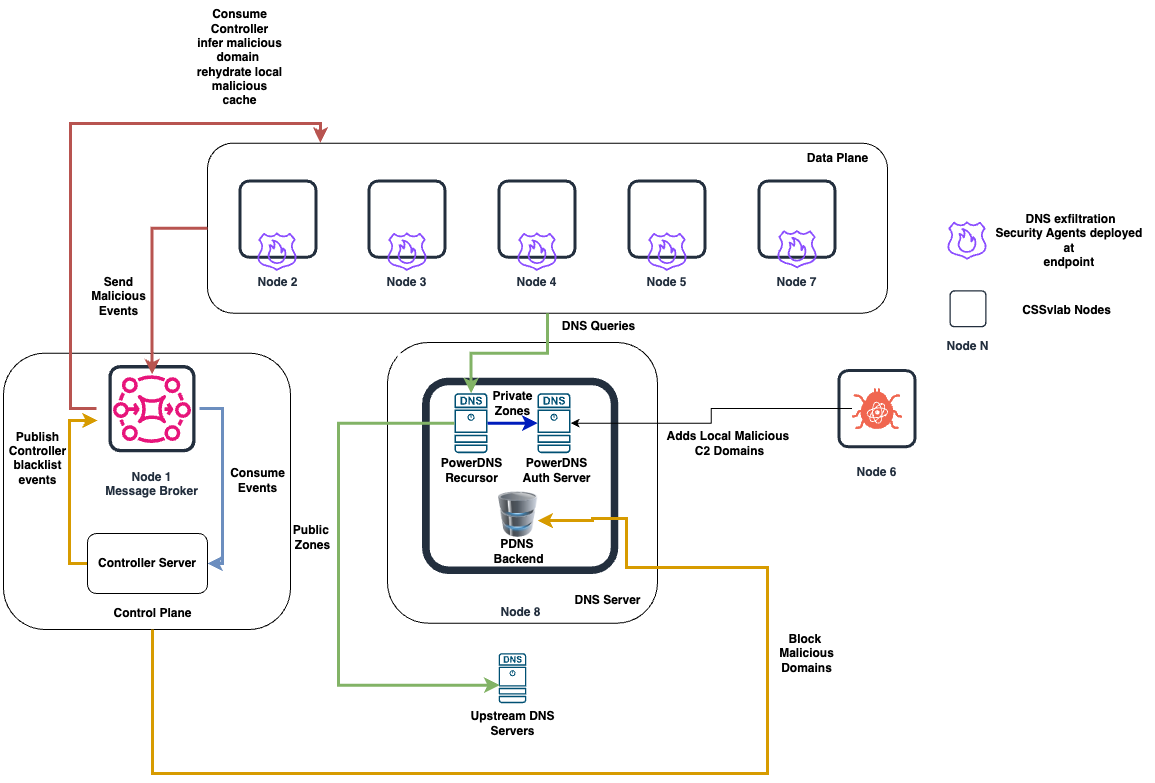
\includegraphics[width=1.0\textwidth]{UWThesis/images/cssvlab-arch.png}
\caption{Security Framework Deployed Architecture over CSSVLAB Nodes}
\label{sec:deployed-arch}
\end{figure}


\section{Evaluations Results}
The evaluation of this security framework is presented for each individual component in the subsequent sections.

\subsection{Data Plane}
The effectiveness of the eBPF node agent at the data plane endpoint is evaluated through quantized deep learning metrics, DNS request throughput comparison across both operational phases (active and passive), and measurement of bandwidth and resource utilization, including CPU and memory usage, as well as kernel event processing throughput. Finally, the agent’s resilience against advanced adversary emulation frameworks is demonstrated using detailed dashboard metrics exported by the eBPF node agent. Performance evaluation is conducted on a single selected node within the data plane running the agent.

\subsubsection{Deep Learning Model Evaluation}
The evaluation of the trained deep learning model was conducted on a dataset of 6 million domains, split into 70\% for training and 15\% each for validation and testing. After training, the model achieved a validation precision of 99.7\%, with loss steadily decreasing per epoch and reaching 0.98\% by the end of training. Given the DNS data exfiltration use case, model performance was primarily evaluated with an emphasis on minimizing false positives. High false positives would not only result in the eBPF node agent dropping benign DNS packets and generating false threat events but could also terminate legitimate  processes introducing operational risks. In contrast, false negatives were deemed less critical, as the agent would allow limited malicious traffic through without taking privilege-level actions. Therefore, precision (TP / [TP + FP]) was prioritized over recall (TP / [TP + FN]). Based on these considerations and a dataset engineered to include a wide range of data obfuscation techniques, the model achieved a high precision of 99.79\% and recall of 99.76\%. For runtime inference via ONNX within the eBPF agent, a decision threshold of 0.98 was selected, as the model demonstrated near-perfect classification (AUC ≈ 1). This performance was largely due to the selected feature set, including Shannon entropy over various encoding and encryption schemes, which enabled effective learning. \hyperref[model_metrics]{Figure 5.1} illustrates the model’s performance on both the training and validation datasets, while \hyperref[fig:model_metrics_quadrant]{Figure 5.3} highlights the improved performance over 25 training epochs.

\begin{table}[H]
\centering
\begin{tabular}{lcc}
\hline
\textbf{Metric} & \textbf{Training} & \textbf{Validation} \\
\hline
Accuracy & 0.9979 & 0.9978 \\
AUC & 0.9997 & 0.9997 \\
Loss & 0.0094 & 0.0089 \\
Precision & 0.9979 & 0.9979 \\
Recall & 0.9979 & 0.9976 \\
% True Positives & 214359.75 & 88966 \\
% True Negatives & 225677.89 & 94631 \\
% False Positives & 440.77 & 188 \\
% False Negatives & 476.13 & 215 \\
\hline
\end{tabular}
\caption{Model Evaluation Metrics}
\label{model-evaluation-metrics}
\end{table}

\begin{figure}[H]
  \centering
  \begin{subfigure}[b]{0.48\textwidth}
    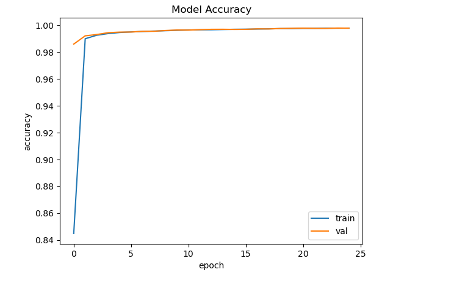
\includegraphics[width=\textwidth]{UWThesis/images/results/model/macc.png}
    \caption{Model Accuracy}
    \label{fig:image1}
  \end{subfigure}
  \hspace{0.02\textwidth}
  \begin{subfigure}[b]{0.48\textwidth}
    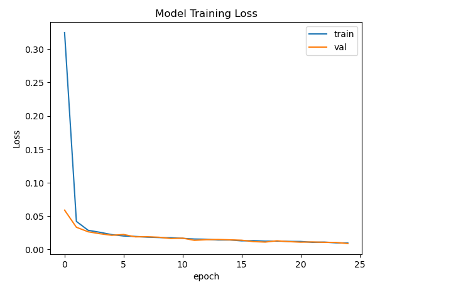
\includegraphics[width=\textwidth]{UWThesis/images/results/model/mloss.png}
    \caption{Model Loss}
    \label{fig:image2}
  \end{subfigure}

  \vspace{0.3cm}

  \begin{subfigure}[b]{0.48\textwidth}
    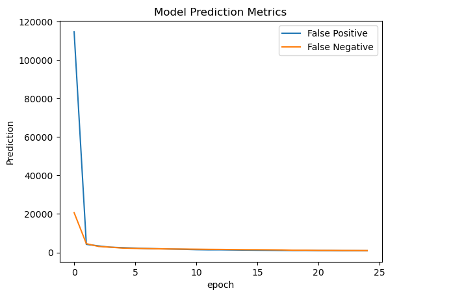
\includegraphics[width=\textwidth]{UWThesis/images/results/model/mpred.png}
    \caption{Model Precision}
    \label{fig:image3}
  \end{subfigure}
  \hspace{0.02\textwidth}
  \begin{subfigure}[b]{0.48\textwidth}
    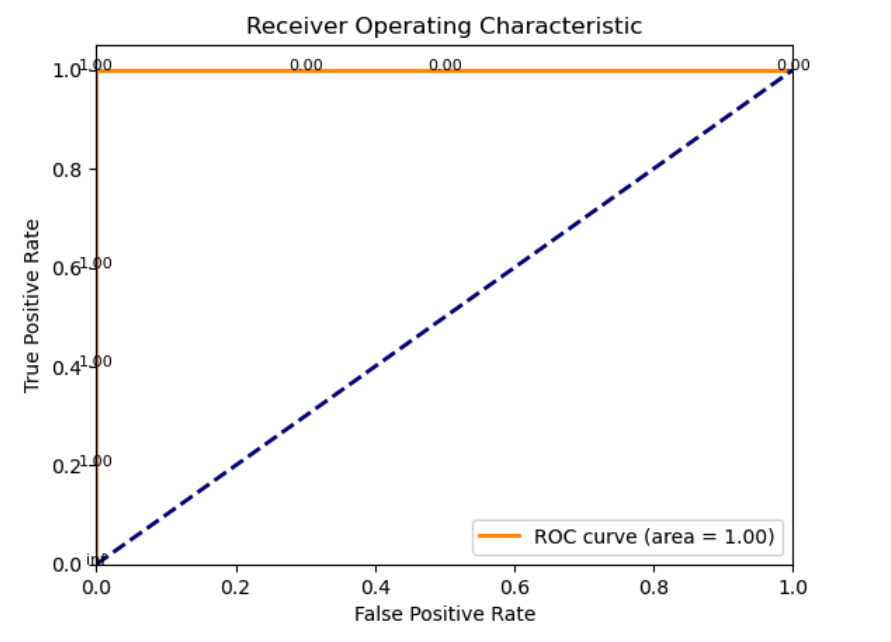
\includegraphics[width=\textwidth]{UWThesis/images/results/model/roc.png}
    \caption{ROC Curve}
    \label{fig:image4}
  \end{subfigure}

  \caption{Model performance metrics: accuracy, loss, precision, and ROC curve}
  % \caption{Model performance across different training epochs}
  \label{fig:model_metrics_quadrant}
\end{figure}


\subsubsection{eBPF Node Agent Request Throughput and Latency Metrics in Active Mode}
The performance of the system was evaluated in active mode by measuring the impact on benign DNS traffic during standard end-to-end resolution—from a userspace process sending DNS requests, through kernel redirection via eBPF programs, to the network device monitored by the agent. For cache hits, the request is matched against the global SLD cache; for cache misses, live ONNX inference is performed. The kernel feature thresholds in the eBPF map were intentionally kept stringent, causing most DNS packets to be flagged as suspicious to stress-test the throughput. Throughput was measured using DNSPerf, which quantifies both request throughput and DNS response success rates. The test locked DNSPerf to send 10,000 DNS requests per second over 20 seconds, monitoring for packet loss. The DNS recursor server assumed to be healthy is running on a Microsoft Hyper-V hypervisor \texttt{hv\_netvsc} virtual driver with NIC supporting a maximum bandwidth of 100 Gbits/sec and running with 8 RX and TX combined resulting in the lack of discrete ring buffers used in kernel for \texttt{AF\_XDP} sockets thereby lacking support \texttt{AF\_XDP} sockets for direct packet injection into TX queues. As a result, the egress path was forced to rely on \texttt{AF\_PACKET}. In the cache-hit scenario (100\% benign SLD matches), throughput ranged from 8,100 to 9,820 DNS requests/sec with zero packet loss as presented \hyperref[fig:throughput_gsld]{Figure 5.3}. Latency ranged from near 0 ms to a maximum of 250 ms per 10k sample \hyperlink{fig:latency_gsld}{Figure 5.5}, validating the lightweight nature of the kernel+userspace eBPF agent pipeline. However, in the cache-miss path requiring live inference, throughput dropped significantly—minimum of 430 and maximum of 520 requests/sec as illustated in \hyperref[fig:throughput_onnx]{Figure 5.4}, with peak latencies up to 750 ms showin in \hyperref[fig:latency_onnx]{Figure 5.6}. Despite this, no packet loss was observed, ensuring reliability. The latency spike is attributed to UNIX domain socket-based communication overhead with the ONNX inference server and Python’s GIL (Global Interpreter Lock), which bottlenecks concurrency—unlike the Go-based core agent that remains highly concurrent and compiled for performance.
It was observed that throughput becomes unstable beyond 5,000 DNS requests/sec, though such traffic volumes typically indicate malicious behavior and can be rate-limited in kernel eBPF programs. Overall, for stress testing over prolonged period of time the agent successfully processed a maximum throughput of 67.3 million DNS requests per hour with no packet loss, all while performing deep parsing across both kernel and userspace.

\begin{figure}[H]
  \centering
  \begin{minipage}[t]{0.47\textwidth}
    \centering
    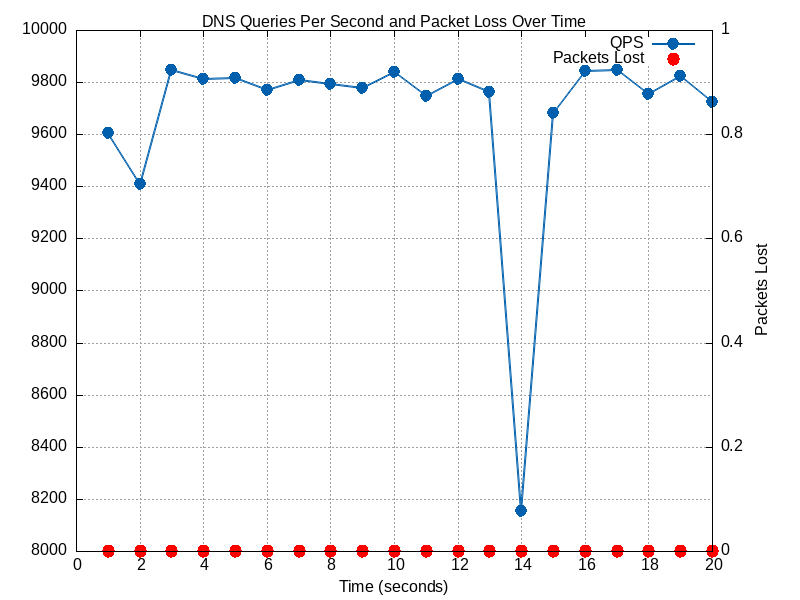
\includegraphics[width=\textwidth]{UWThesis/images/results/throughput/throughput_active_gsld_lru.png}
    \caption{eBPF Agent: DNS Throughput for GSLD LRU Hit (10k req/s)}
    \label{fig:throughput_gsld}
  \end{minipage}
  \hfill
  \begin{minipage}[t]{0.47\textwidth}
    \centering
    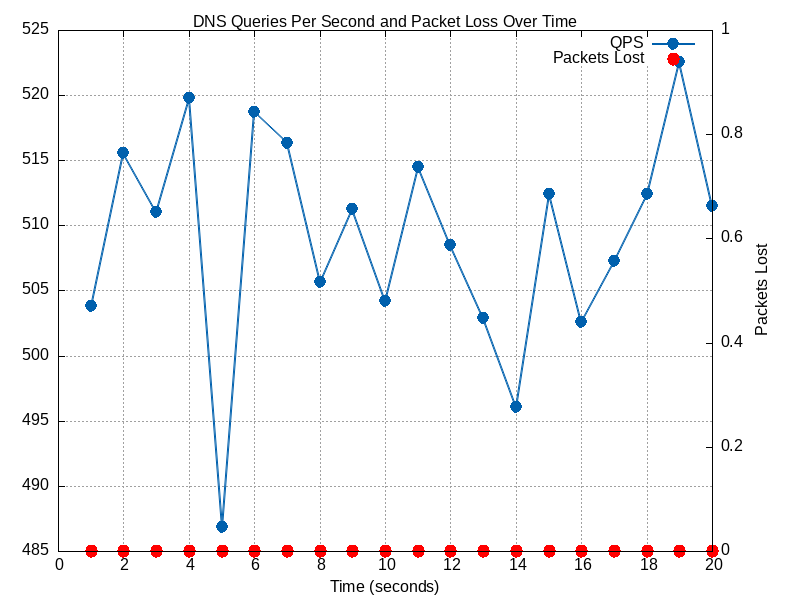
\includegraphics[width=\textwidth]{UWThesis/images/results/throughput/throughput_active_onnx.png}
    \caption{eBPF Agent: DNS QPS, GSLD LRU Miss, ONNX (10k req/s)}
    \label{fig:throughput_onnx}
  \end{minipage}

  \vspace{1cm} % Increased spacing before lower images

  \begin{minipage}[t]{0.47\textwidth}
    \centering
    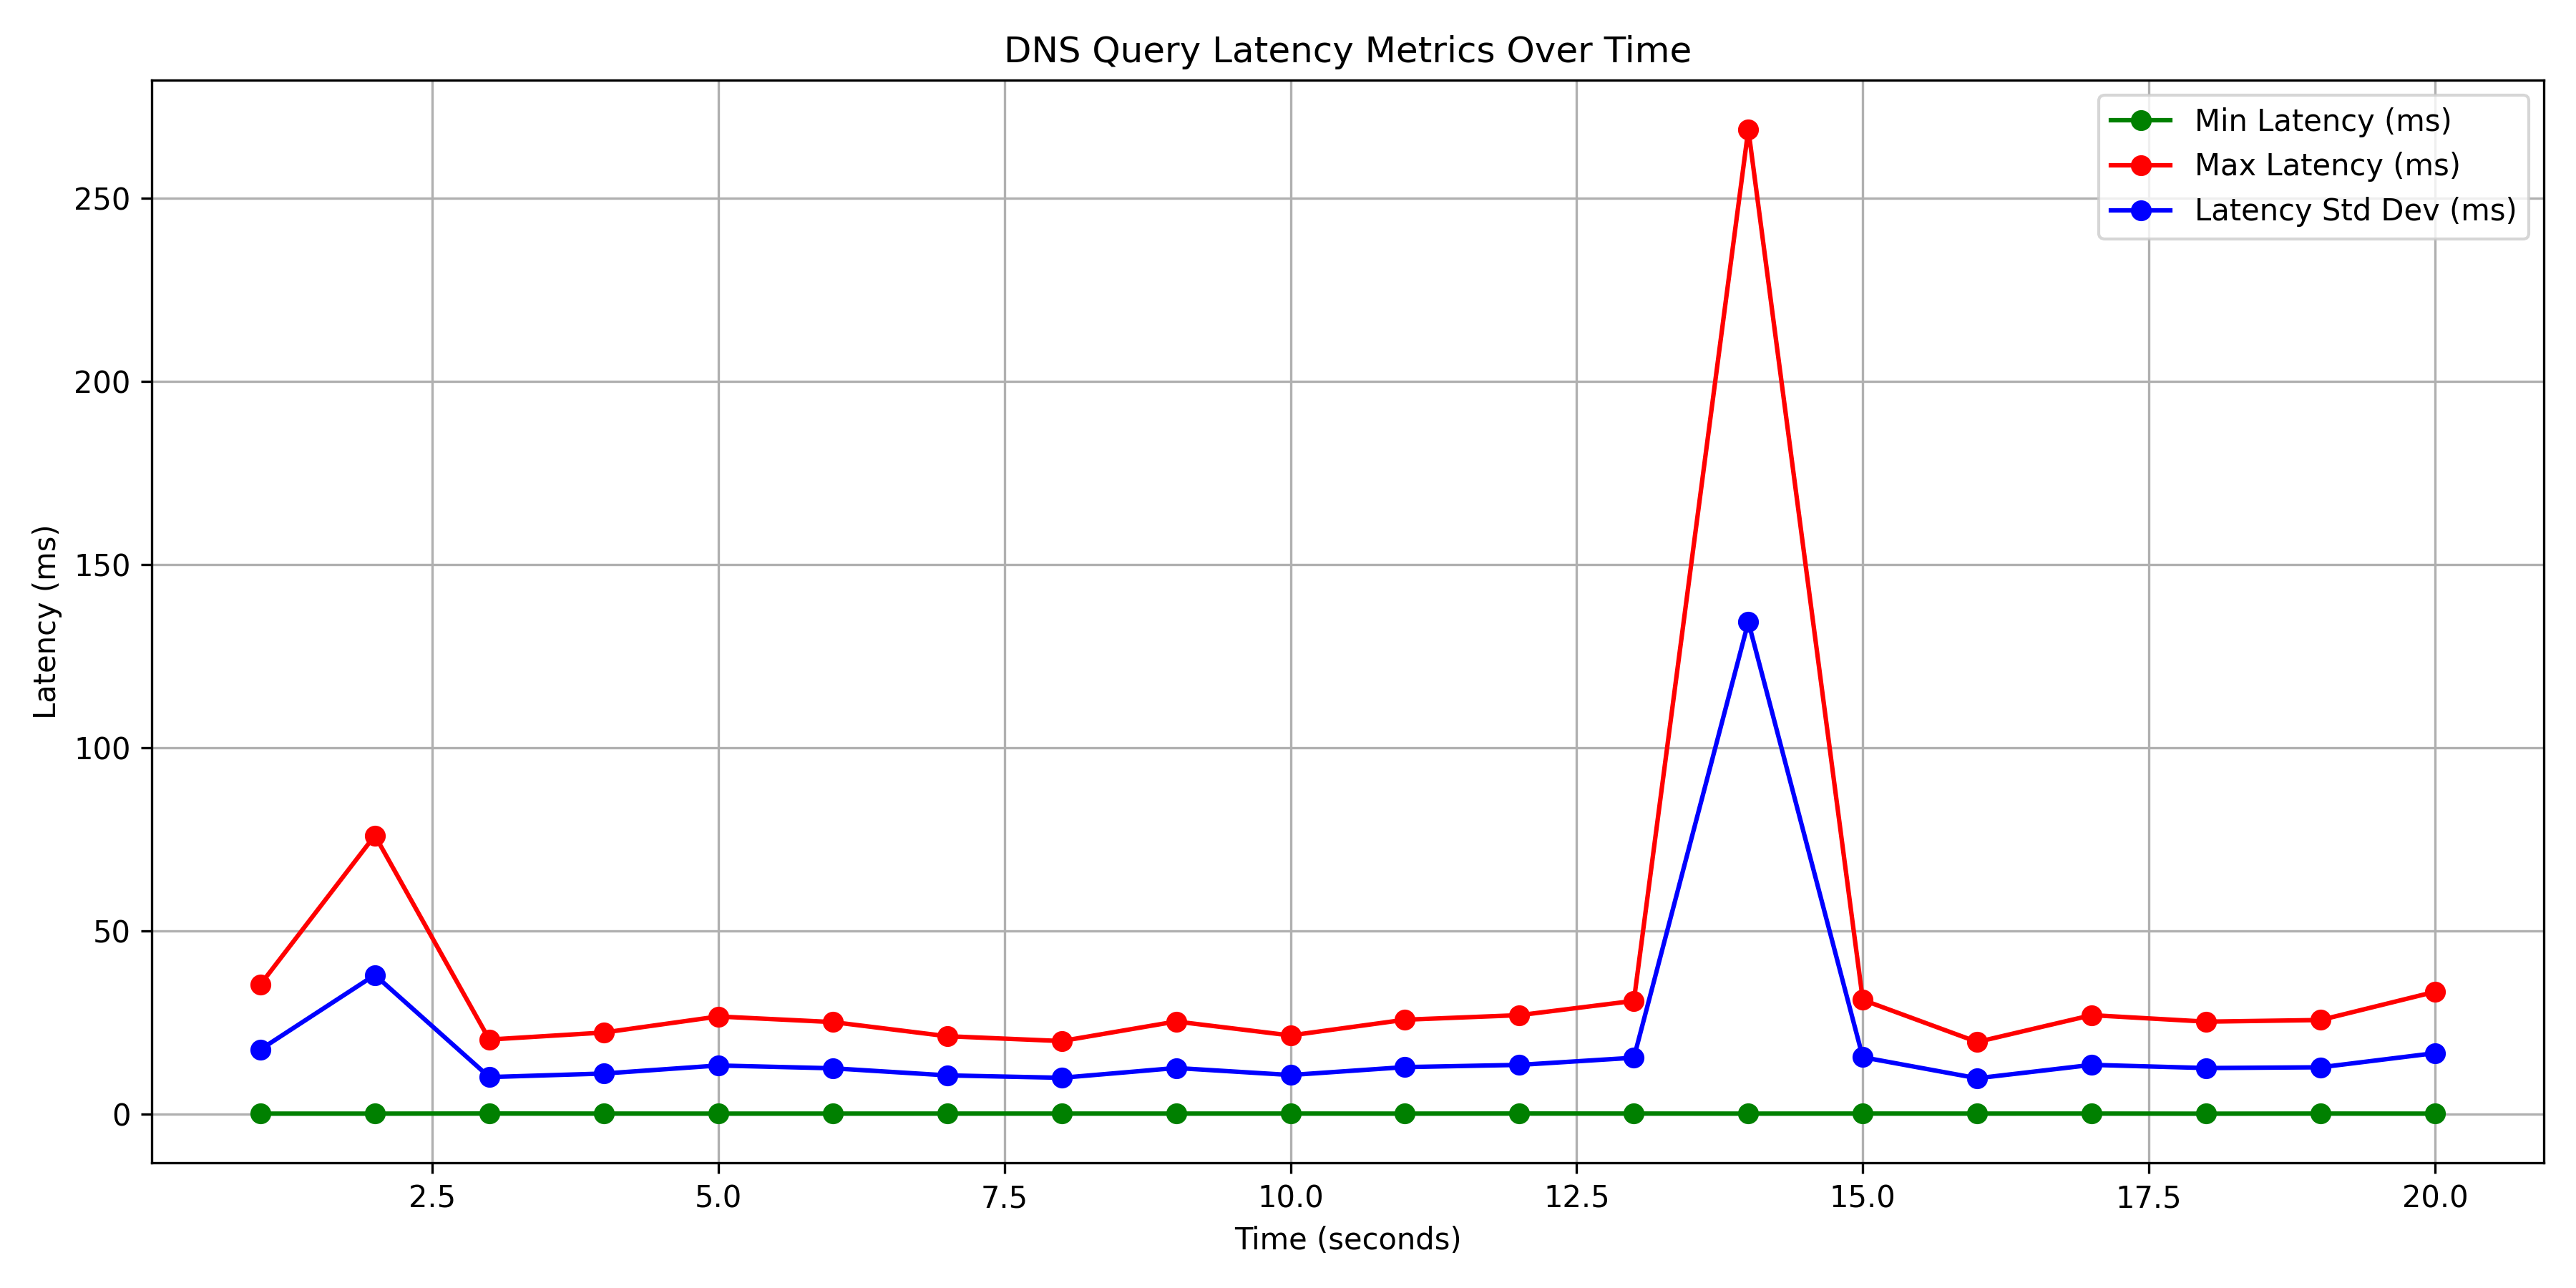
\includegraphics[width=\textwidth,height=0.68\textwidth]{UWThesis/images/results/throughput/latency_metrics_gsld.png}
    \caption{eBPF Agent: DNS Latency for GSLD LRU Hit (10k req/s)}
    \label{fig:latency_gsld}
  \end{minipage}
  \hfill
  \begin{minipage}[t]{0.47\textwidth}
    \centering
    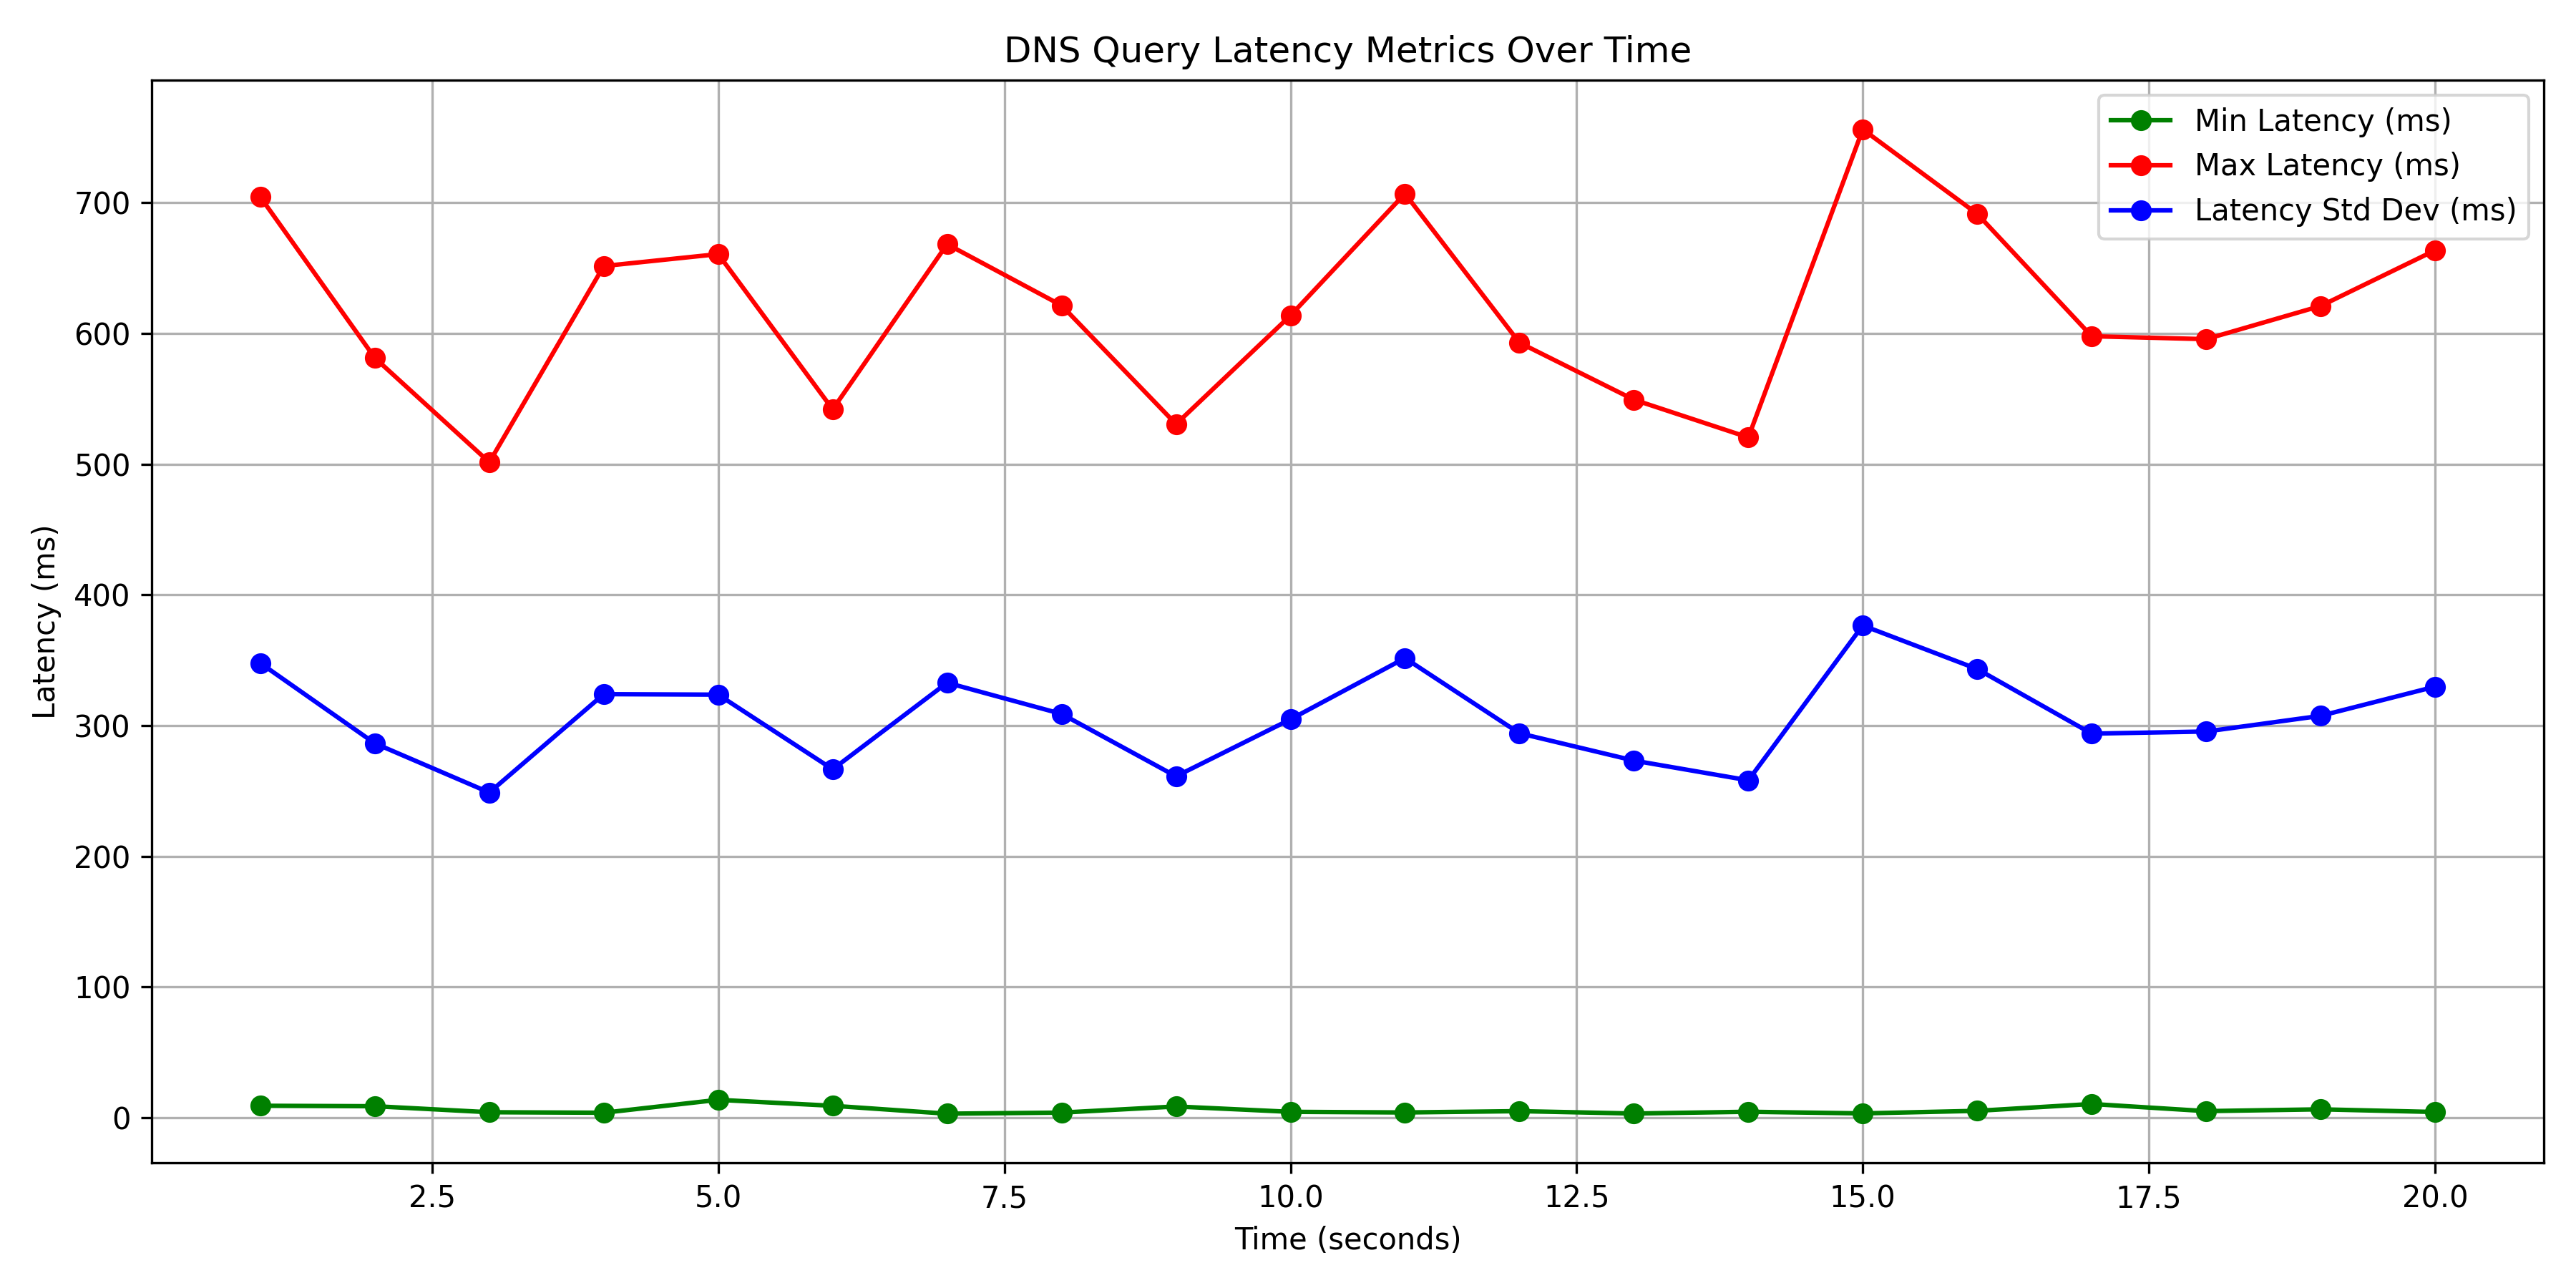
\includegraphics[width=\textwidth,height=0.68\textwidth]{UWThesis/images/results/throughput/latency_metrics_onnx.png}
    \caption{eBPF Agent: DNS Latency, GSLD LRU Miss, ONNX (10k req/s)}
    \label{fig:latency_onnx}
  \end{minipage}
\end{figure}

\subsubsection{eBPF Node Agent Request Throughput and Latency Metrics in Passive Mode}
The primary evaluation metric in passive mode is the volume of DNS-based data exfiltration successfully prevented before terminating malicious processes. In this mode, the agent employs a clone-and-redirect mechanism, allowing original DNS packets to pass through while kernel programs inspect traffic for signs of malicious activity. Upon detection, the kernel notifies the userspace agent to kill the responsible process. Traditional throughput and latency are not emphasized; instead, performance is measured by how effectively the system detects and halts beaconing implants that transmit data over DNS, often across random UDP ports. \hyperref[fig:data_loss_prev]{Figure 5.7} illustrates the total volume of exfiltrated data stopped by the eBPF agent prior to process termination. For example, DNSCat2, configured with a 20-second beaconing interval and exfiltrating via various DNS record types (MX, TXT, CNAME, HTTP, SRV, etc.), demonstrated the system’s strength in delaying termination just enough to observe beaconing patterns—empowering administrators to tune termination thresholds for maximum insight.

\begin{figure}[H]
  \centering
  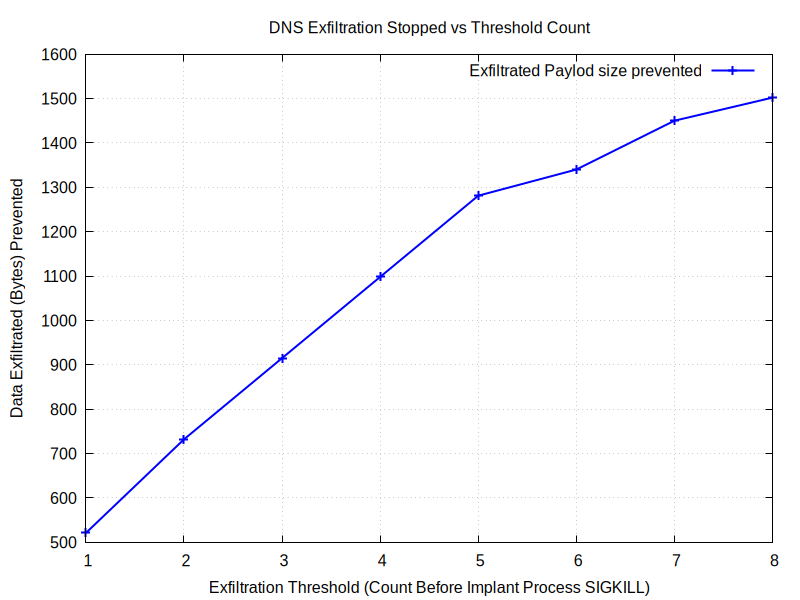
\includegraphics[width=0.6\textwidth]{UWThesis/images/results/data_loss_passive/exfil_stopped_passive_data_prevented_and_kill.png}
\caption{eBPF Agent preventing passive DNS exfiltration across varying thresholds prior SIGKILL}
  \label{fig:data_loss_prev}
\end{figure}

% \begin{table}[ht]
% \centering
% \caption{Evaluation of DNS Exfiltration and C2 Tool Detection}
% \begin{tabular}{|l|l|p{5cm}|p{4.5cm}|}
% \hline
% \textbf{Tool Name} & \textbf{Exfiltration Technique} & \textbf{Measured Results} & \textbf{Comments} \\
% \hline
% Iodine & DNS Tunneling & Around 100\% accuracy in detecting and preventing tunnels in real time (all virtual interfaces, any random port) & -- \\
% \hline
% DNScat2 & DNS C2 & Around 100\% accuracy in stpping breaches and terminating C2 channels in real time (all virtual interfaces, any random port) & Detects both slow-rate and fast-rate exfiltration \\
% \cline{2-4}
% & DNS Tunneling & Similar accuracy; detects SOCKS5, SSH, HTTP, or any protocol tunnels over DNS (standard and non-standard ports) & -- \\
% \hline
% Sliver & DNS C2 & Similar accuracy; detects SOCKS5, SSH, HTTP, or any protocol tunnels over DNS (standard and non-standard ports) & -- \\
% \hline
% Dns Exfiltrator & Raw Exfiltration & Fully detects and prevents high-throughput exfiltration with killing the DET python processes & -- \\
% \hline
% \end{tabular}
% \label{tab:tool-evaluation}
% \end{table}


\subsubsection{eBPF Node Agent Resource Usage}
The performance of the eBPF node agent was closely monitored while running at the endpoint in the data plane, with resource usage measured in terms of memory and CPU utilization. During a 10-second DNSPerf benchmark at 10,000 DNS req/sec, with the agent in active mode redirecting all packets to userspace, the agent consumed approximately 310 MB of memory for the main process. This includes heap memory, as all LRU maps loaded by agent's process for fast lookups. At a higher throughput of 100,000 DNS requests/sec, memory usage remained nearly the same, peaking at 350 MB. \hyperref[fig:mem10k]{Figure 5.8},  \hyperref[fig:mem100k]{Figure 5.9} illustrates the memory usage for previously explained DNS request throughput. Throughout the benchmark, CPU usage by the agent process remained under 2\%, and memory usage for agent for an idle system reaching close to 120 MB demonstrating that the agent is extremely lightweight from CPU needs, with no impact on other processes running at the endpoint. In addition, the agent binary compiled size with all the  explained features is around 22 MB on ARM and 24 MB on x86\_64 architectures ensuring there is minimal storage impact on the endpoint caused due to eBPF node agent.

\begin{figure}[H]
  \centering
  \begin{minipage}[b]{0.48\textwidth}
    \centering
    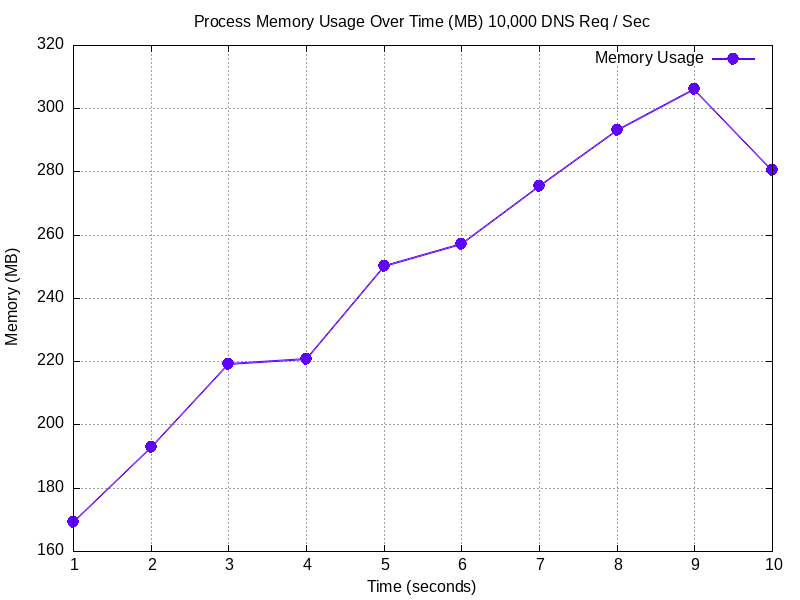
\includegraphics[width=\textwidth]{UWThesis/images/results/mem_usage/memory_usage10k.png}
    \caption{eBPF Agent Process Memory Usage for 10k DNS req/sec}
    \label{fig:mem10k}
  \end{minipage}
  \hfill
  \begin{minipage}[b]{0.48\textwidth}
    \centering
    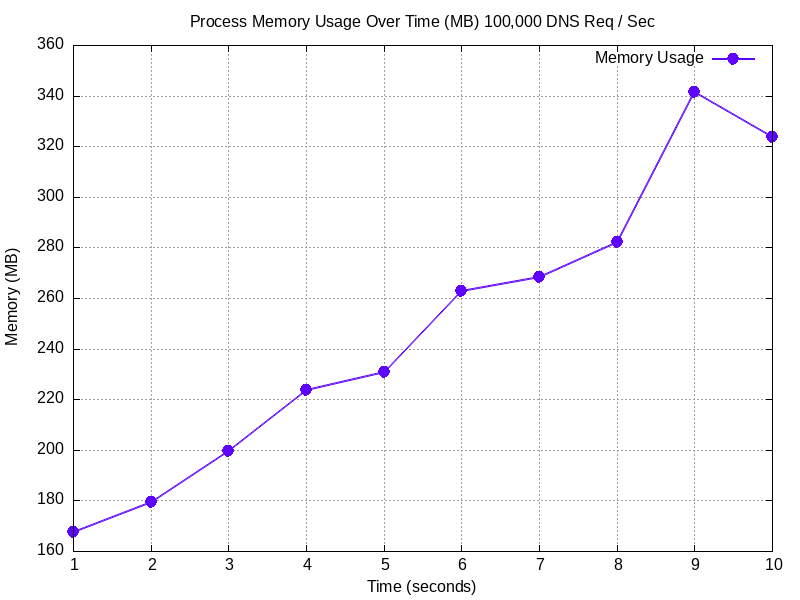
\includegraphics[width=\textwidth]{UWThesis/images/results/mem_usage/memory_usage_mass100k.png}
    \caption{eBPF Agent Process Memory Usage for 100k DNS req/sec}
    \label{fig:mem100k}
  \end{minipage}
\end{figure}

\subsection{eBPF Node Agent effectiveness over DNS exfiltration tools}
The eBPF node agent was evaluated across all data plane endpoints against widely used, high-reputation DNS-based C2 frameworks commonly leveraged by red teams in production for penetrationt testing. Testing focused on detecting and disrupting C2 and exfiltration activities tunneled over DNS. The CSSVLAB06 node acted as the primary attacker, issuing commands through a DNS server to the targeted data plane nodes.
The Sliver C2 framework, developed by BishopFox, was assessed not only for basic data exfiltration but also for its support of advanced C2 operations. These included remote shell access, remote code execution, file transfers, remote port forwarding, and establishing persistent backdoors via dynamically opened ports—all encapsulated within DNS traffic. The eBPF agent enforced kernel-level mitigation from the very first C2 command, immediately breaking the communication channel, forcing implant retries, and ultimately terminating the process. This applied to both beaconing and session-based implants.
Although Sliver does not support DNS tunneling over randomized UDP ports, the agent’s ability to handle transport-layer obfuscation was evaluated using dnscat2, which does support such techniques. The same set of C2 vectors was executed with the agent running in both active and passive modes. In both cases, the agent successfully enforced mitigation policies, resulting in full session teardown with no exfiltration.
For raw data exfiltration scenarios, tools like DET, which lack UDP port randomization capabilities, were used. With the agent operating in active mode, raw exfiltration attempts were immediately blocked with zero data loss, and the offending processes were terminated. Additionally, DNS tunneling tools such as Iodine were tested for their ability to tunnel arbitrary protocols through DNS. The agent effectively intercepted and dropped the encapsulated payloads, confirming its ability to prevent a broad spectrum of DNS-based exfiltration and tunneling strategies. \hyperref[tab:dns-framework-coverage]{Figure 5.10} illustrates the  attack vectors prevented. 

\newpage
\begin{figure}[H]
  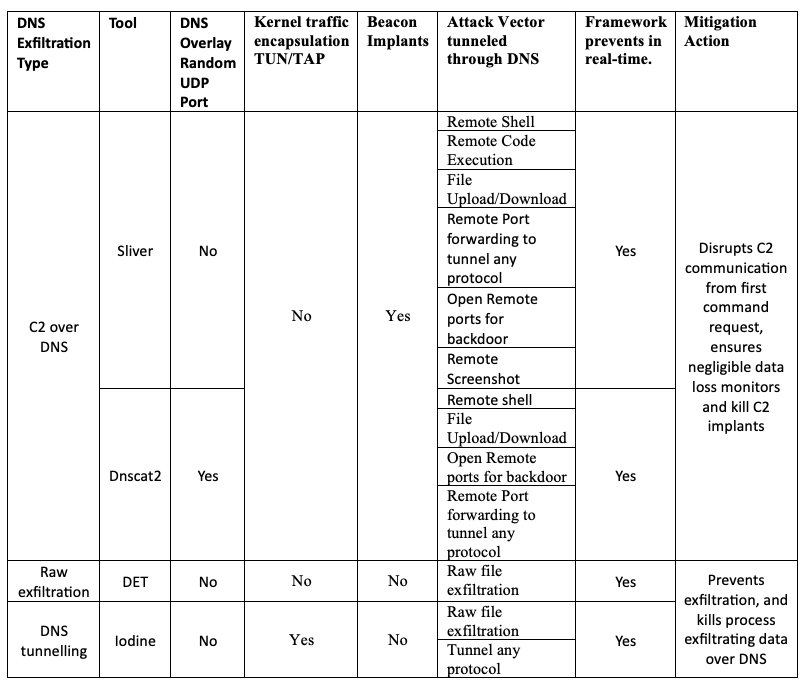
\includegraphics[width=1\textwidth]{UWThesis/images/results/C2_exfil_strength.png}
  \caption{Framework Coverage Against Real-World DNS-Based C2 and Exfiltration Tools}
\label{tab:dns-framework-coverage}
\end{figure}

\subsubsection{Control Plane}
The evaluation of the controller’s stateless server focuses on its effectiveness in accurately consuming threat events streamed from data plane nodes to a Kafka topic, blacklisting domains in RPZ, and redistributing those events to data plane nodes to rehydrate their malicious domain caches.The \hyperref[fig:controller_metric]{Figure 5.11} figure illustrates the structure of threat events streamed from eBPF agents in the data plane, serialized as JSON and published to a Kafka topic. These events are consumed by the controller and used to blacklist domains in the RPZ zone of the DNS server. The \hyperref[fig:controller_aware_metric]{Figure 5.12} figure shows how the controller republishes structured threat data back to the Kafka topic for data plane nodes to consume. As previously explained, the controller’s published events also include Layer 3 (IPv4/IPv6) addresses of remote C2 nodes. This enables agents in the data plane to enforce cross-protocol correlation by dynamically injecting L3 filtering rules into the kernel. This design not only blocks DNS-based DGA communication but also halts all protocol-level traffic to malicious IPs, offering strong protection from distributed threats and elevating system-level security enforcement directly inside the kernel.


\begin{figure}[H]
  \centering
  \begin{minipage}[t]{0.47\textwidth}
    \centering
    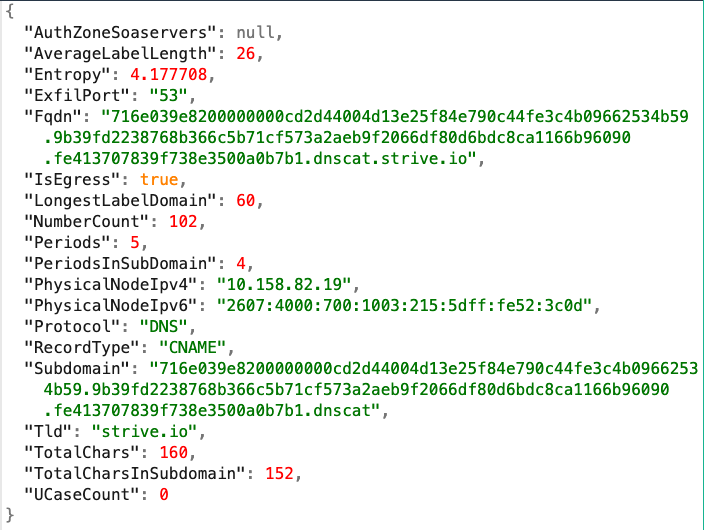
\includegraphics[width=\textwidth]{UWThesis/images/results/controller_consumed_threat_event.png}
\caption{Controller consumed threat event}
  \label{fig:controller_metric}
  \end{minipage}
  \hfill
  \begin{minipage}[t]{0.47\textwidth}
    \centering
    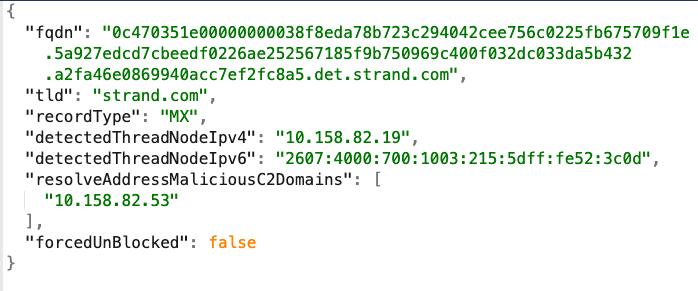
\includegraphics[width=\textwidth]{UWThesis/images/results/controller_informed_threat_event.png}
    \caption{Controller streamed threat event}
     \label{fig:controller_aware_metric}
  \end{minipage}
\end{figure}

\subsubsection{Distributed Infrastructure}
The performance evaluation of the distributed infrastructure focuses solely on the DNS server, specifically assessing the throughput impact of the Lua-based interceptor running on the PowerDNS Recursor. As shown in \hyperref[fig:throughput_gsld_tcp]{Figure 5.13}, the server was benchmarked under a sustained load of 10,000 DNS requests per second. Due to the reuse of the same inference server design as in the data plane—along with reliance on UNIX sockets for inter-process communication and Python’s internal concurrency limitations—throughput dropped to as low as 490 DNS requests per second. Latency measurements, illustrated in \hyperref[fig:throughput_onnx_tcp]{Figure 5.14}, peaked at approximately 750ms, with the mean deviation stabilizing around 380ms.
All TCP traffic benchmarks in the kernel were conducted with \texttt{TCP\_FAST\_OPEN} enabled, allowing application data to be sent with the initial SYN packet. This reduced the impact of the TCP 3-way handshake on throughput and enabled accurate latency measurements for DNS-over-TCP traffic.
In addition, \hyperref[fig:dns_rpz]{Figure 5.15} shows the resulting blacklisted domains stored in the PowerDNS GPSQL backend. The controller supplements this list with additional metadata, allowing for selective unblocking of domains based on operational requirements. In such cases, the controller initiates a forced reprogramming of all data plane nodes, overriding local suspicion heuristics to permit DNS traffic for the specified domain.



\begin{figure}[H]
  \centering
  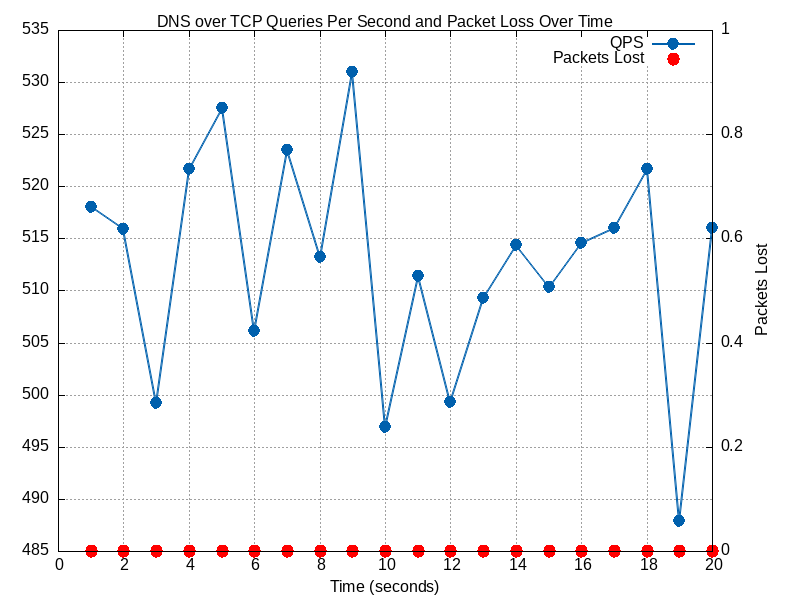
\includegraphics[width=0.8\textwidth]{UWThesis/images/results/tcp/throughput_active_onnx_tcp.png}
  \caption{DNS Server Throughput for 10k DNS req/s over TCP}
  \label{fig:throughput_gsld_tcp}
\end{figure}

\begin{figure}[H]
  \centering
  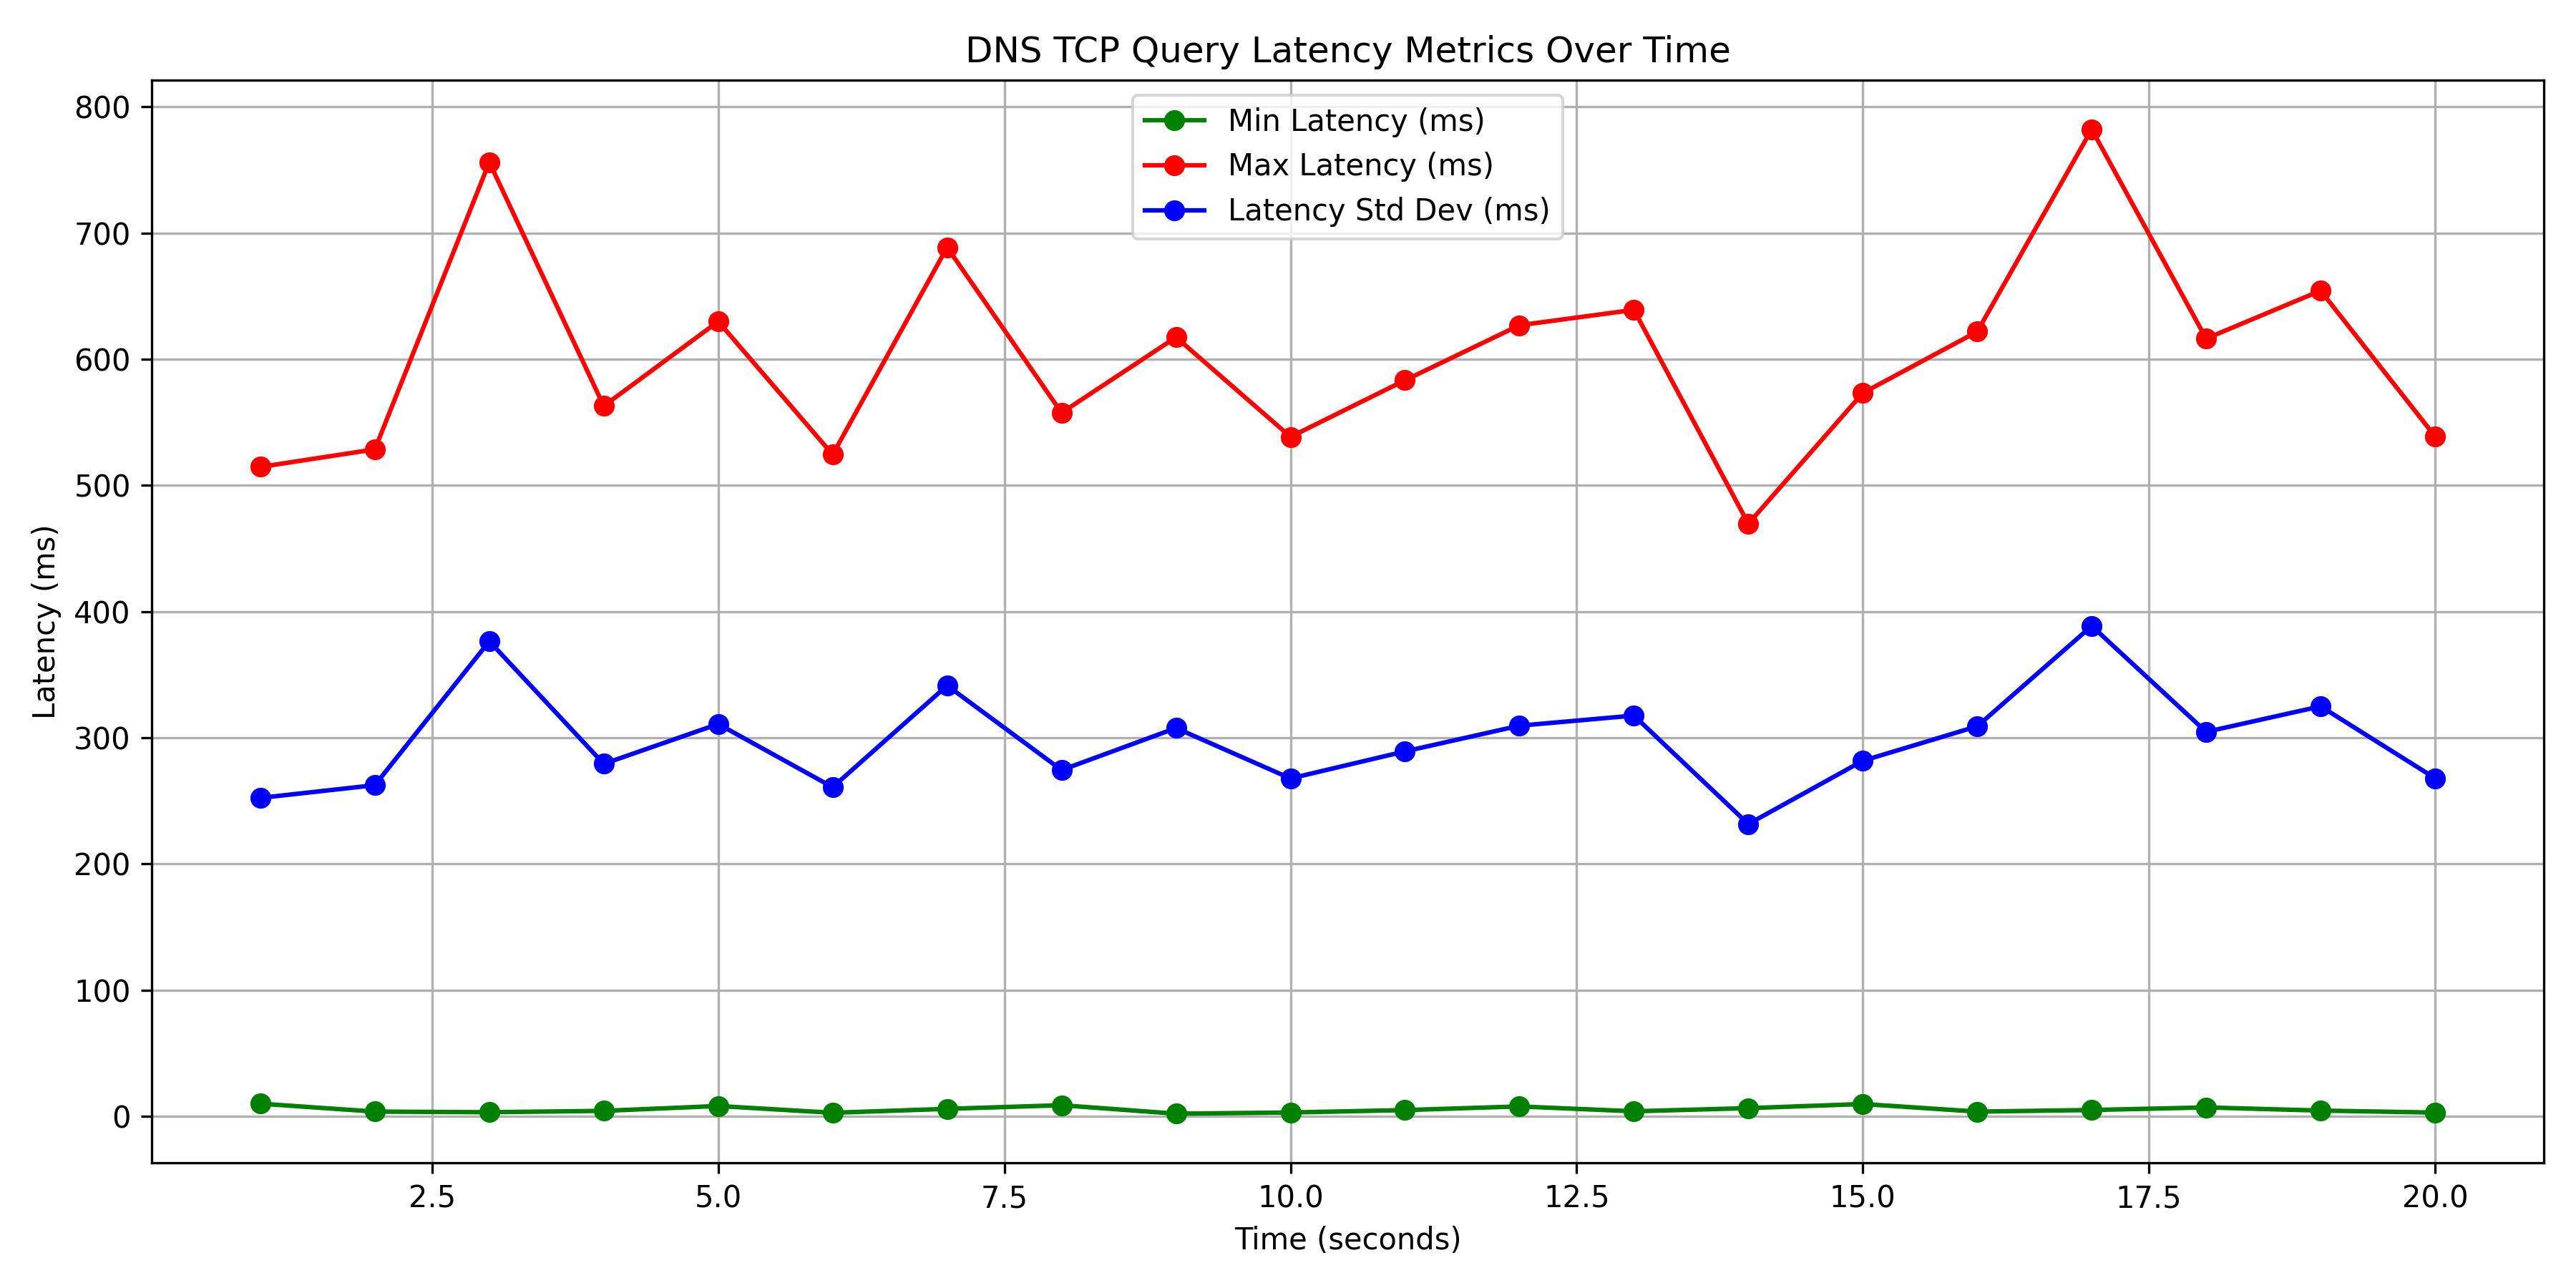
\includegraphics[width=0.8\textwidth]{UWThesis/images/results/tcp/latency_metrics_onnx_tcp.png}
  \caption{DNS Server Latency for 10k DNS req/s over TCP}
  \label{fig:throughput_onnx_tcp}
\end{figure}



\begin{figure}[H]
  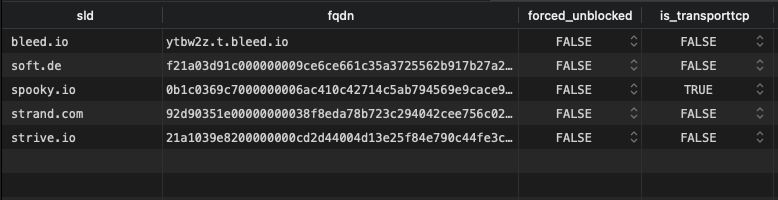
\includegraphics[width=1\textwidth]{UWThesis/images/results/dns_rpz_blacklist.png}
\caption{Blacklisted domains in RPZ zone in DNS server}
  \label{fig:dns_rpz}
\end{figure}





% Data plane:
% 1. Model Metrics 
% 2. Threougput metrcis 
%     Active phase (en / dis) (gld / inferencing need) (covers latency)
%     Passive Mode (en) (inferencing) (covers latency)
%     Kernel eBPF events / I/O usage
%     node agent userspace memory usage
%     Data loss prior removal (line chart)
%     Effectiveness over all tools  (active)
%         (dnscat2, sliver, iodine, DET, nuages)
%     Data plane promethesu metric dashboards

% Control plane:
% 1. 

% Distributed infra
% 1. Security over TCP , blacklist domain 
    

\chapter{Conclusion}
This chapter concludes the whole paper by summarizing the contents and give future directions.


\section{Summary}
This security framework significantly advances the state of the art by developing a novel architecture for preventing data exfiltration over DNS, directly addressing critical gaps left by traditional approaches. Existing literature and solutions for DNS exfiltration prevention remain largely stagnant, centered around centralized detection and userspace anomaly detection systems or proxied DPI which are inherently inadequate and lack the strength to stop sophisticated DNS-based exfiltration, especially those leveraging C2 implants or APT malware once the system is compromised. In contrast, this framework introduces a new paradigm: kernel-enforced endpoint security. It acts as a privileged layer beneath existing endpoint security solutions, enabling strict enforcement in tandem with userspace agents. With security code running inside the kernel, these agents at the endpoint possess unprecedented defensive strength stopping and killing even the most advanced forms of DNS C2 implants, including remote code execution, shellcode exploits, port forwarding, reverse tunnels, and SOCKS tunnels in real-time often used by most reputable adversary emulation tools actively used in production by red teamers.
Furthermore, by combining a layered, system-security-first approach with an endpoint-centric design, it significantly enhances endpoint security in ways that were never possible when relying solely on userspace. The result is a deeply integrated, system-level defense that delivers unprecedented visibility into OS activity, enables intelligent threat hunting, and robustly thwarts advanced exfiltration techniques in real time. This work have been recognized by the primer Linux kernel community for innovations been presented at the most selective and prestigious kernel networking and security conferences. In addition, it is set to be presented at one of the world’s largest security conferences, showcasing innovation to advance DNS security with the goal of making DNS a safe protocol and protecting enterprises from these evolving DNS threats. The below points summarizes the strengths of the security framework.

\begin{itemize}[itemsep=1pt,parsep=0pt]
    \item \textbf{Instant DNS C2 Disruption} – Immediately blocks DNS-based command-and-control channels upon initiation, stopping covert communication at the source.

    \item \textbf{Active Implant Detection \& Termination} – Detects malicious processes abusing DNS for exfiltration or remote control and terminates them in real time.

    \item \textbf{Tunnel and Encapsulation-Aware Defense} – Eliminates DNS tunnels, protocol-agnostic payload encapsulation, including DNS overlay over random UDP ports.

    \item \textbf{Reverse and Port-Forwarded Tunnel Neutralization} – Stops reverse shells, SOCKS5 proxies, and port-forwarded advanced commands tunneled inside DNS between compromised and attacker-controlled nodes.

    \item \textbf{DGA Mitigation with Deep Observability} – Dynamically blacklists  domains, reprogram agents in dataplane and enforce layer 3 network policies for cross protocol coorelation.

    \item \textbf{Rich metrics and system observability} – Exports rich metrics to Prometheus for visibility of system level observability at each endpoints.

    \item \textbf{Horizontal Scalability} – Designed with focus on horizontal scalability as in production cloud environments 

    \item \textbf{Kernel-Level Endpoint Attribution} – Provides fine-grained OS and process-level insight, attributing DNS exfiltration attempts to specific binaries and users.
\end{itemize}

\section{Limitation and Future Work}

\subsection*{Limitations}

\begin{itemize}[itemsep=1pt,parsep=0pt]
  % \item \textbf{Limited Protocol Coverage:} Current implementation focuses primarily on DNS exfiltration; while not on DNS-over-HTTP, DoT (DNS-over-TLS), and encrypted channels require additional enforcement mechanisms.

  \item \textbf{High Latency for deep learning model inferencing:} UNIX socket IPC, and python limitation for pure concurrency significantly reduced throughput and increased latency. 
  % \item \textbf{Partial DNS Parsing:} The DNS parser implemented in kernel currently covers only key sections of the protocol. Further parsing of DNS message structure (e.g., full RR parsing, EDNS, DNSSEC) is pending.

  \item \textbf{Absence of Encrypted Exfiltration Detection:} The framework does not yet support prevention of exfiltration over encrypted DNS channels such as DoT or DoH.

  \item \textbf{Absence of Encrypted Encapsulated Tunnels:} The framework does not support prevention of exfiltration over encrypted tunnels relying on kernel \texttt{xfrm} such as wireguard, OpenVPN, IPSec. 

  \item \textbf{Basic Throughput Control:} Egress rate limiting is not yet adaptive to prevent mass throughput or volume exfiltration all inside kernel TC. 
\end{itemize}

\subsection*{Future Work}

\begin{itemize}[itemsep=1pt,parsep=0pt]
  \item \textbf{Extend Support for DNS-over-TCP and Encrypted Tunnels:} Implement detection and blocking for exfiltration of DNS over TCP in kernel eBPF kernel programs replicating TCP state machine coupled with envoy as an L7 userspace proxy for analysis

  \item \textbf{Migration away from Python inference server:} Migrate the python ONNX inference to rust, with a wasm (web assembly) module for faster inferencing compared to interpreted languages.

  \item \textbf{Add In-Kernel TLS Fingerprinting:} Integrate TLS fingerprinting (e.g., JA3/JA4) using eBPF to detect encrypted DNS exfiltration or covert TLS channels over wireguard / mTLS.

  % \item \textbf{Enhance DNS Protocol Parsing:} Expand in-kernel DNS parser to cover full protocol depth, including additional sections and response types.

  % \item \textbf{DPI Optimization Using Mathematical Methods:} Improve efficiency of in-kernel DPI using optimized computation strategies like Newton-Raphson approximations for better performance under high load.

  \item \textbf{XDP-Based Flood Prevention:} Introduce XDP ingress filtering inside kernel to mitigate NXDOMAIN-based DNS water torture and DNS amplification attacks on the endpoint.

  \item \textbf{Rate-Limiting Based on Volume and Throughput:} Integrate egress \texttt{TC CLSACT QDISC}-based dynamic rate limiting via token bucket algorithm implementation through kernel BPF timers to prevent high-throughput DNS data breaches completely inside kernel.

  \item \textbf{Layered Cloud and Kubernetes Defense:} Deploy policy enforcement layers across Kubernetes orchestrated environments (L3/L7 filtering via CNI to drop in userspace) and public cloud cross protocol access control list defending all nodes behind firewall.

  % \item \textbf{XDR/EDR Telemetry Integration:} Export metrics to enterprise security platforms for enriched threat correlation, visibility, and response automation.
\end{itemize}



\chapter{Appendix}

The source code for the security framework is open source and licensed under AGPLv3 license and is available at https://github.com/Synarcs/DNSObelisk.

\section{Appendix A}
This section focuses on providing additional details of the eBPF node agents in data plane.

\subsection{eBPF programs additional implementation details}
This subsection details the internals of the kernel implementation insdie eBPF programs built over the TC layer.

\begin{figure}[H]
    \centering
    \begin{minipage}{0.48\textwidth}
        \centering
        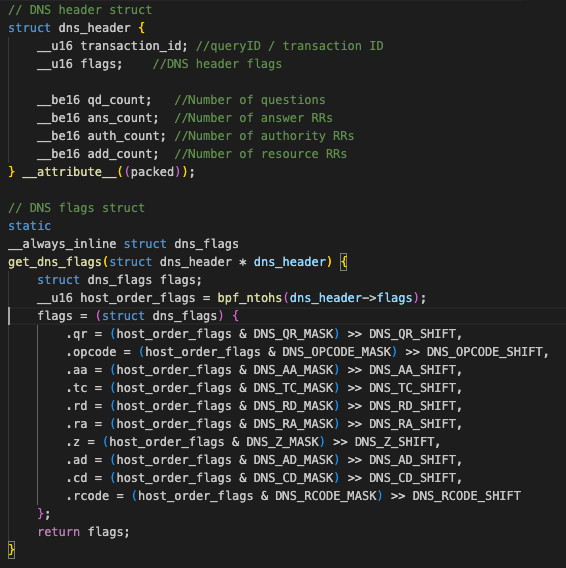
\includegraphics[width=\textwidth]{UWThesis/images/code/c1.png}
        \caption{DNS Protocol Header definitions and parsing in kernel}
        \label{fig:c1}
    \end{minipage}
    \hfill
    \begin{minipage}{0.48\textwidth}
        \centering
        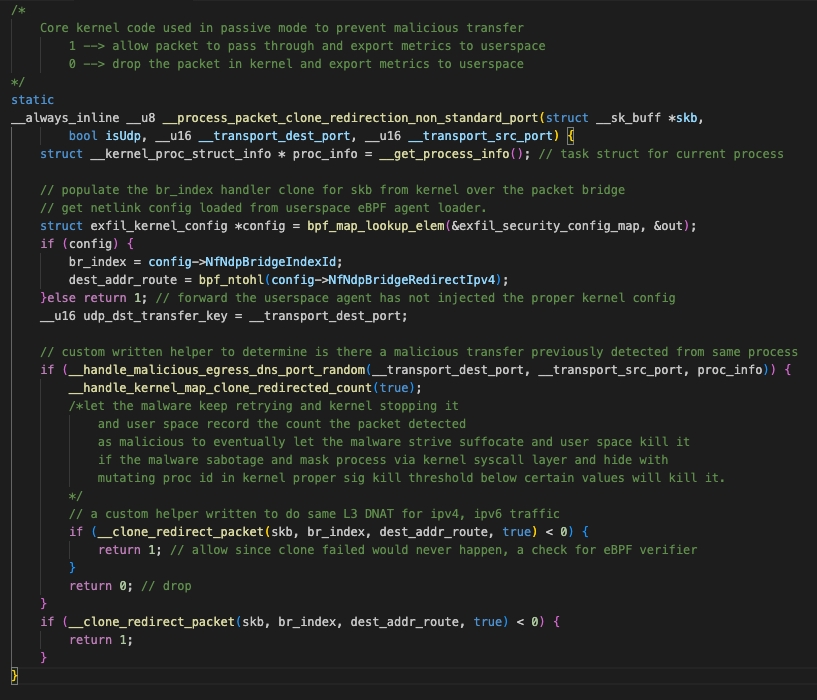
\includegraphics[width=\textwidth]{UWThesis/images/code/passive.png}
        \caption{Agent Passive mode operation in kernel}
        \label{fig:passive}
    \end{minipage}
\end{figure}

\begin{figure}[H]
    \centering
    \begin{subfigure}[t]{0.48\textwidth}
        \centering
        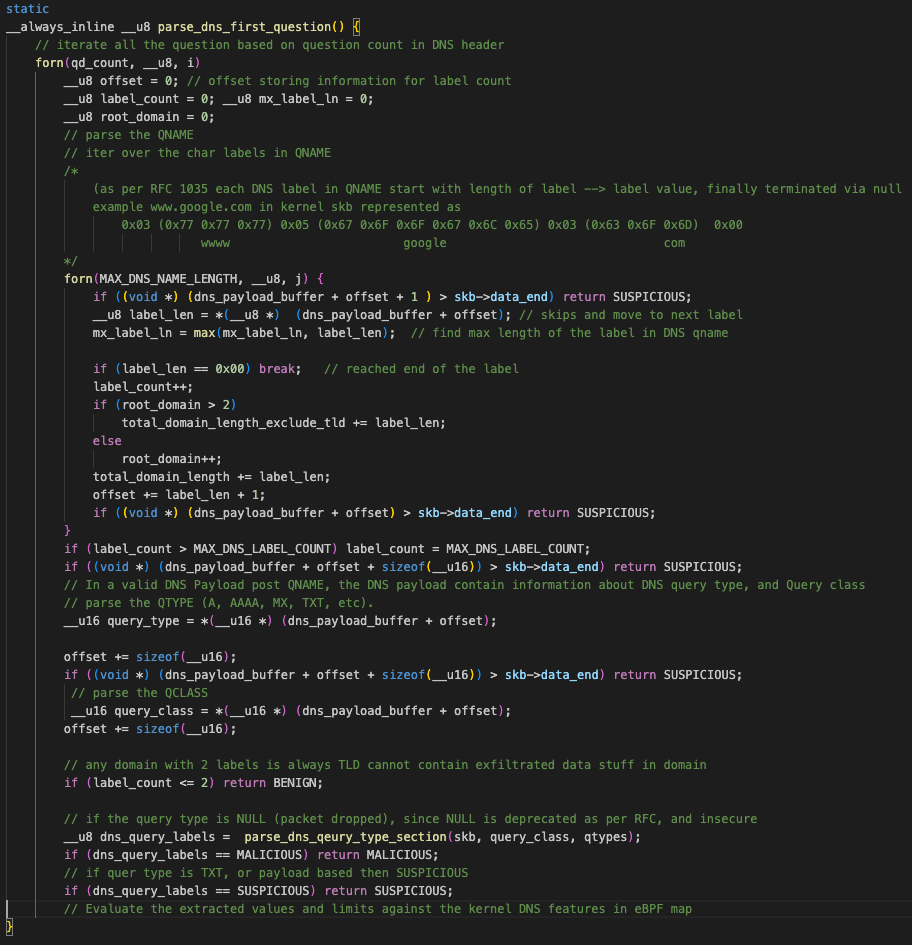
\includegraphics[width=\linewidth]{UWThesis/images/code/dns_parse.png}
        \caption{Raw parsing DNS questions in kernel}
        \label{fig:c2}
    \end{subfigure}
    \hfill
    \begin{subfigure}[t]{0.48\textwidth}
        \centering
        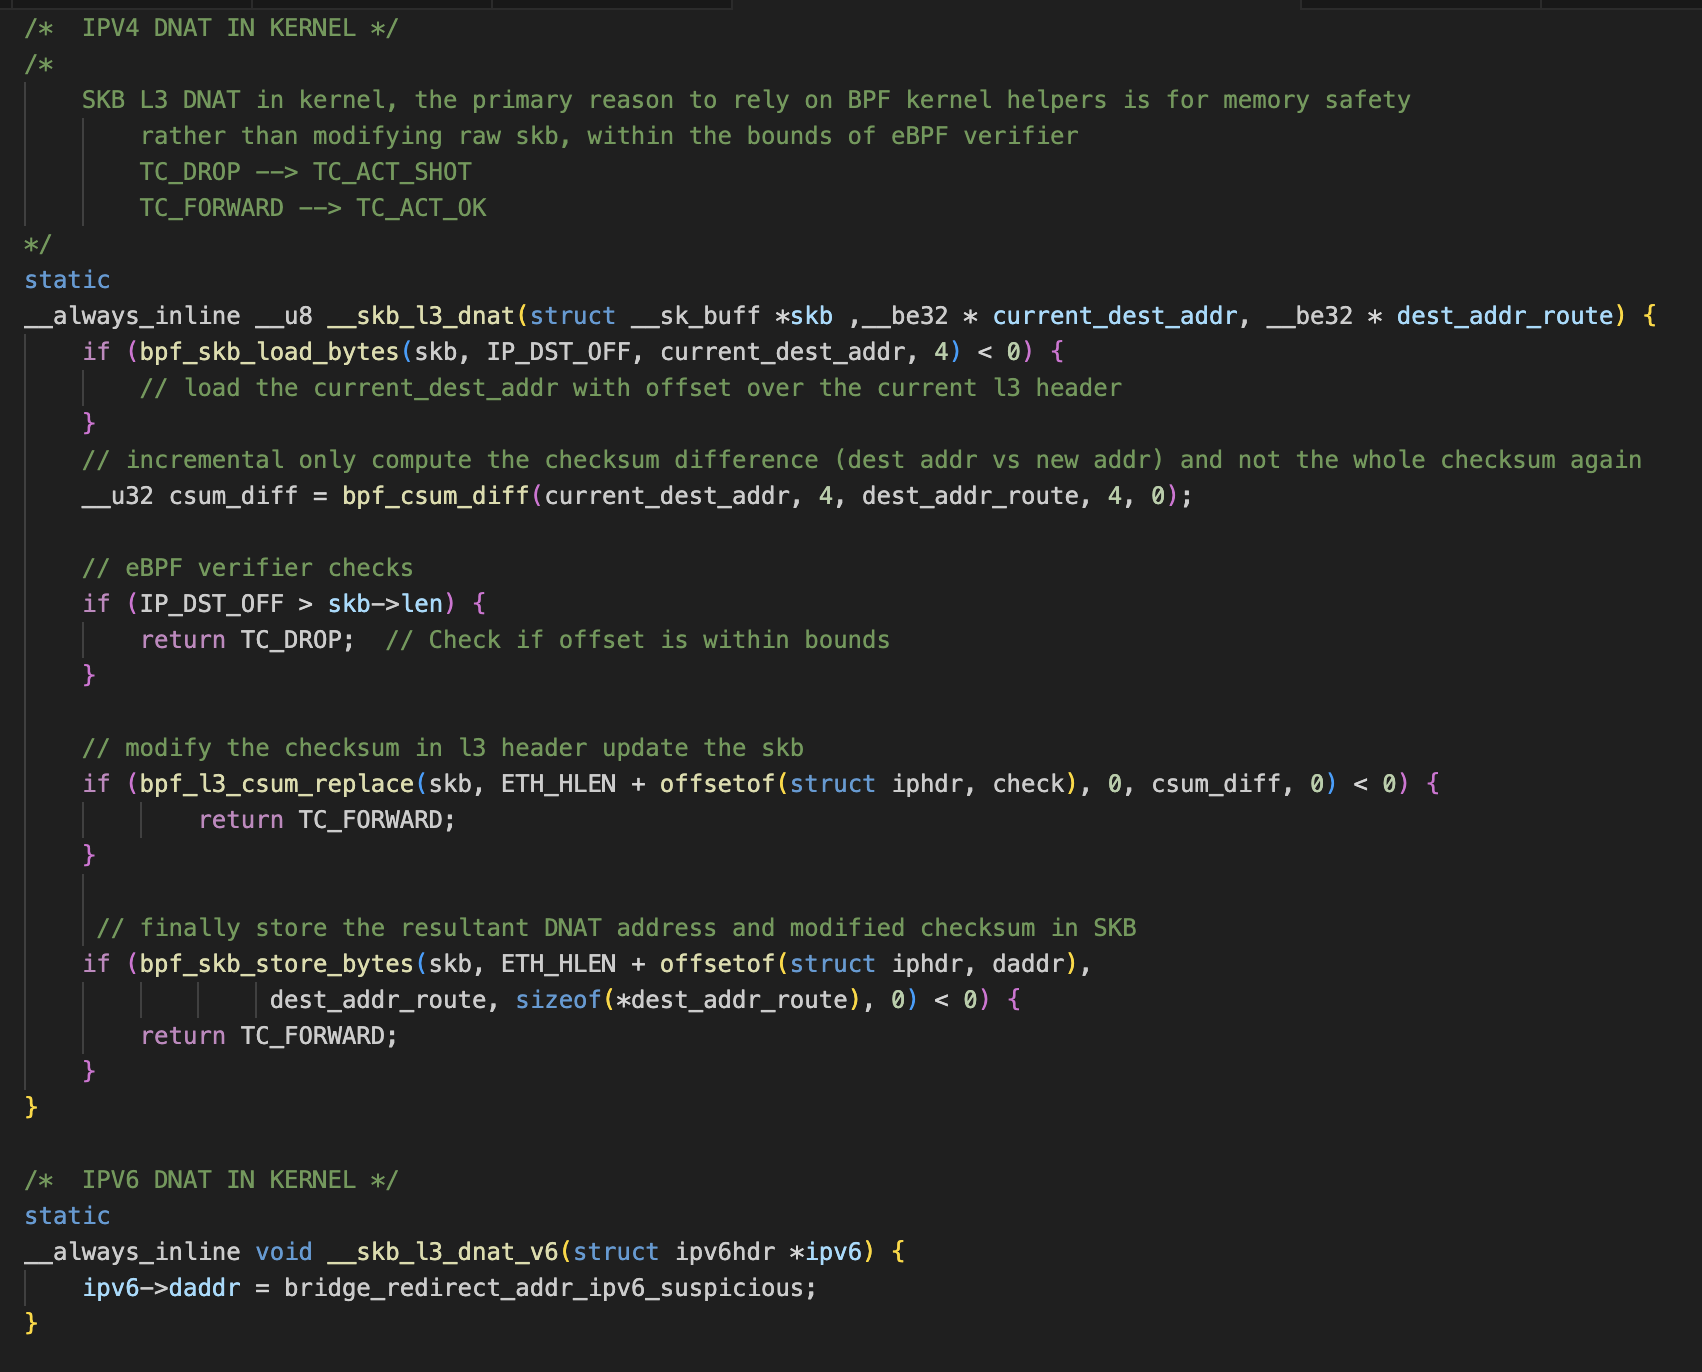
\includegraphics[width=\linewidth]{UWThesis/images/code/l3_dnat.png}
        \caption{In kernel implementation of L3 DNAT for IPv4 / IPv6 traffic}
        \label{fig:l3dnat}
    \end{subfigure}
    \caption{Side-by-side view of C2 detection and L3 DNAT handling.}
    \label{fig:combined}
\end{figure}


\begin{figure}[H]
    \centering
    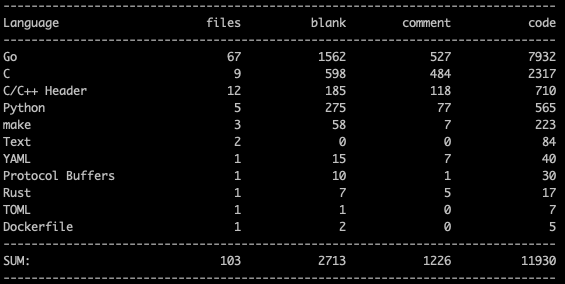
\includegraphics[width=0.5\linewidth]{UWThesis/images/code/Loc/dataplane_loc.png}
    \caption{Lines of Code across Data Plane}
    \label{fig:loc-1}
\end{figure}

\subsection{eBPF programs integrity, security and integration with kernel LSM}


\subsection{Instructions for compiling and deploying the eBPF node agent at the endpoint}


\section{Appendix B}

\begin{figure}[H]
    \centering
    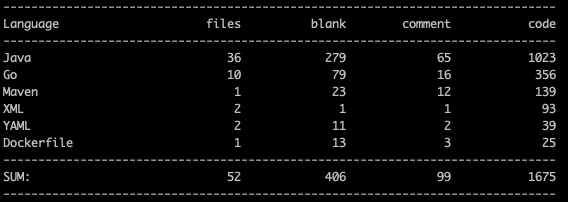
\includegraphics[width=0.5\linewidth]{UWThesis/images/code/Loc/controlplane_loc.png}
    \caption{Lines of Code across Control Plane}
    \label{fig:loc-2}
\end{figure}


\section{Appendix C}


\begin{figure}[H]
    \centering
    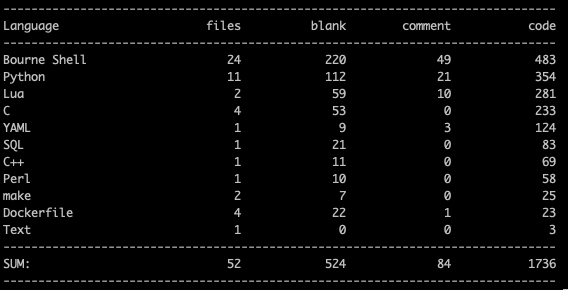
\includegraphics[width=0.5\linewidth]{UWThesis/images/code/Loc/infra_loc.png}
    \caption{Lines of Code across Distributed Infrastructure}
    \label{fig:loc-3}
\end{figure}




\begin{longtable}{|p{4cm}|p{10cm}|}
\hline
\textbf{Metric} & \textbf{Description} \\
\hline
\texttt{DNSFeatures} & Metadata of detected DNS exfiltration packets, including extracted features. \\
\hline
\texttt{Tunnel Interface Process Info} & Tracks kernel netlink events for virtual network device creation, linked to the process that created them (UID, GID, PID). \\
\hline
\texttt{DPI\_Redirect\_Count} & Packet redirection count by kernel DPI logic in active mode. \\
\hline
\texttt{DPI\_Clone\_Count} & Count of cloned packets redirected for inspection in passive mode. \\
\hline
\texttt{DPI\_Drop\_Count} & Total packets dropped by kernel DPI logic. \\
\hline
\texttt{MaliciousProcTime} & Start time and duration the malicious process was alive before termination. \\
\hline
\texttt{CPU Usage} & CPU utilization of the eBPF node agent in userspace. \\
\hline
\texttt{Memory Usage} & RAM usage in MB or percentage of total memory used by the eBPF node agent. \\
\hline
\texttt{DNS Redirect and Processing Time} & In active mode, tracks time from kernel redirection to userspace sniffing, model inference or cache lookup, then resend if benign or block if malicious. \\
\hline
\caption{eBPF Node Agent exported metrics in both active and passive modes}
\label{sec:dp_ebpf_node_metrics}
\end{longtable}





\begin{figure}[H]
  \centering

  % Row 1
  \begin{subfigure}[b]{0.48\textwidth}
    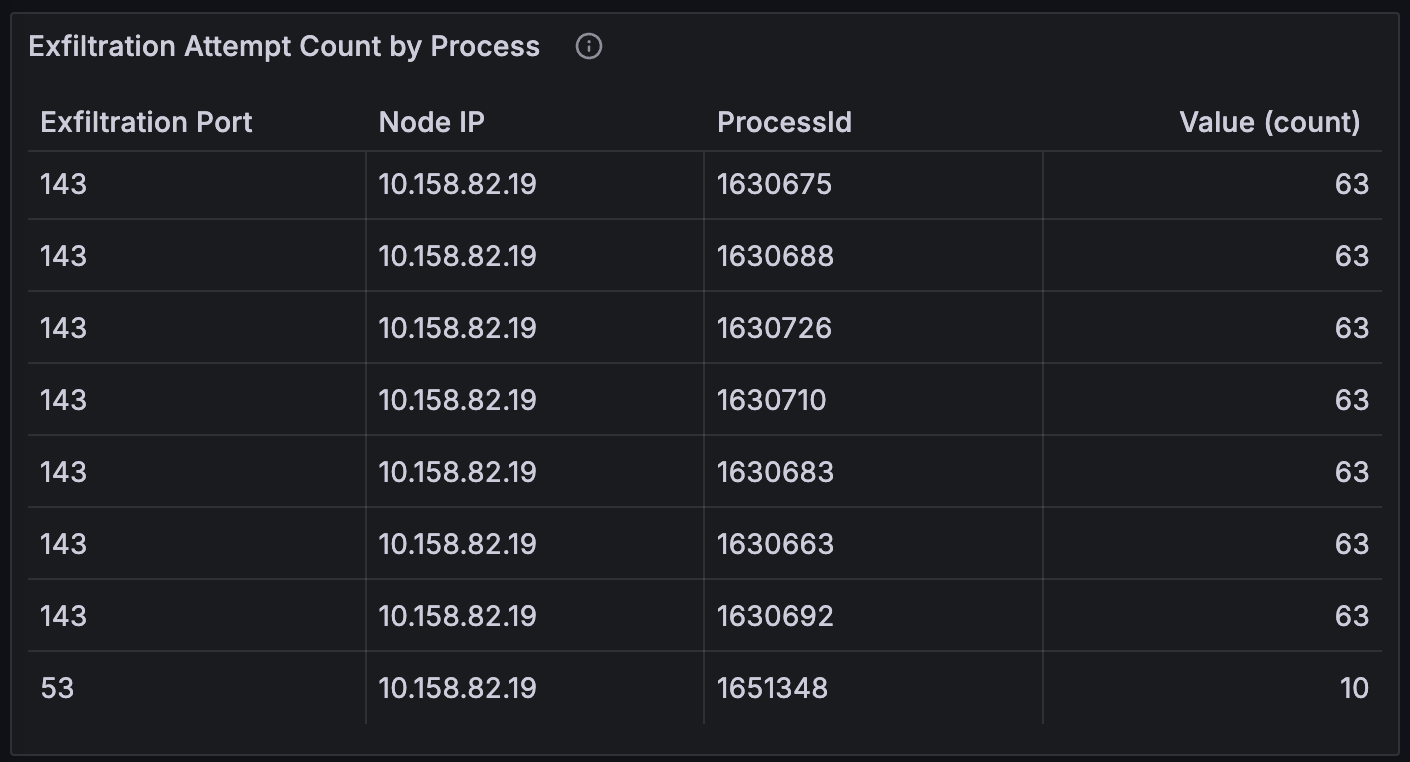
\includegraphics[width=\textwidth]{UWThesis/images/results/metrics/exfiltration attempts prevented per process.png}
    \caption{Exfiltration Attempts Prevented per Process}
  \end{subfigure}
  \hfill
  \begin{subfigure}[b]{0.48\textwidth}
    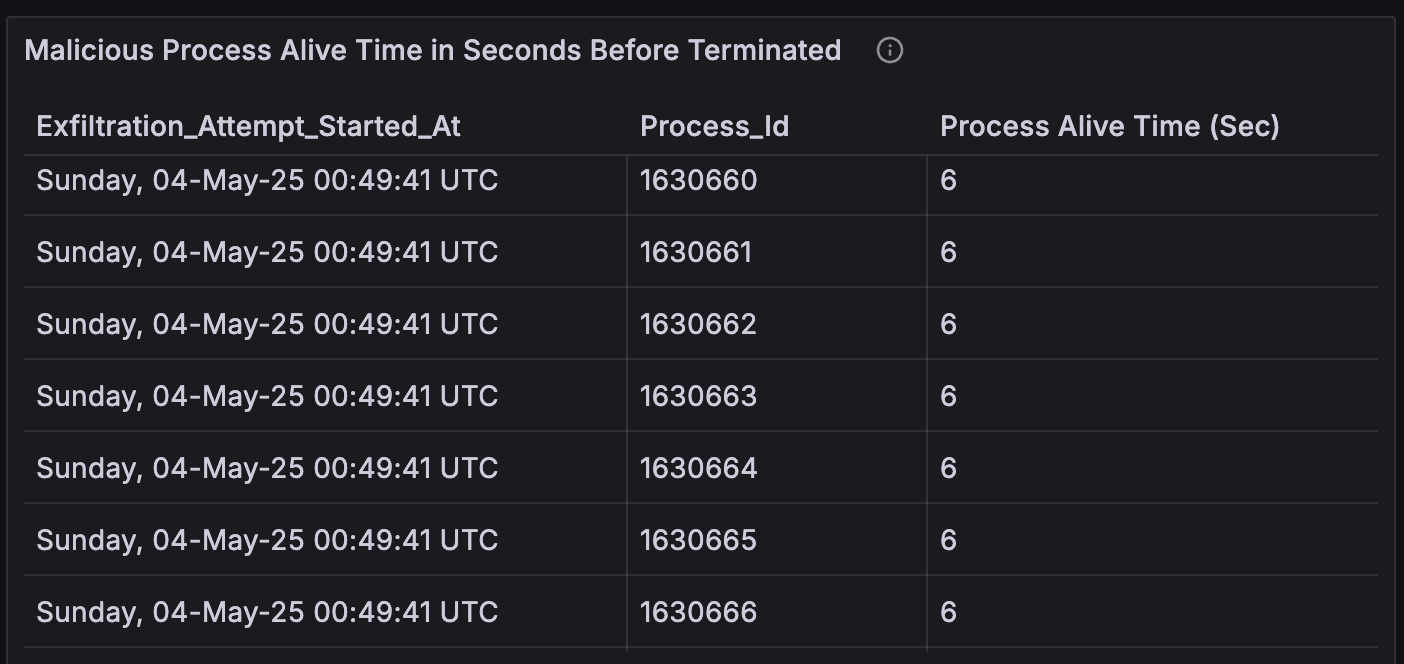
\includegraphics[width=\textwidth]{UWThesis/images/results/metrics/process alive time prior kill.png}
    \caption{Process Alive Time Before Termination}
  \end{subfigure}

  \vspace{0.5cm}

  % Row 2
  \begin{subfigure}[b]{0.48\textwidth}
    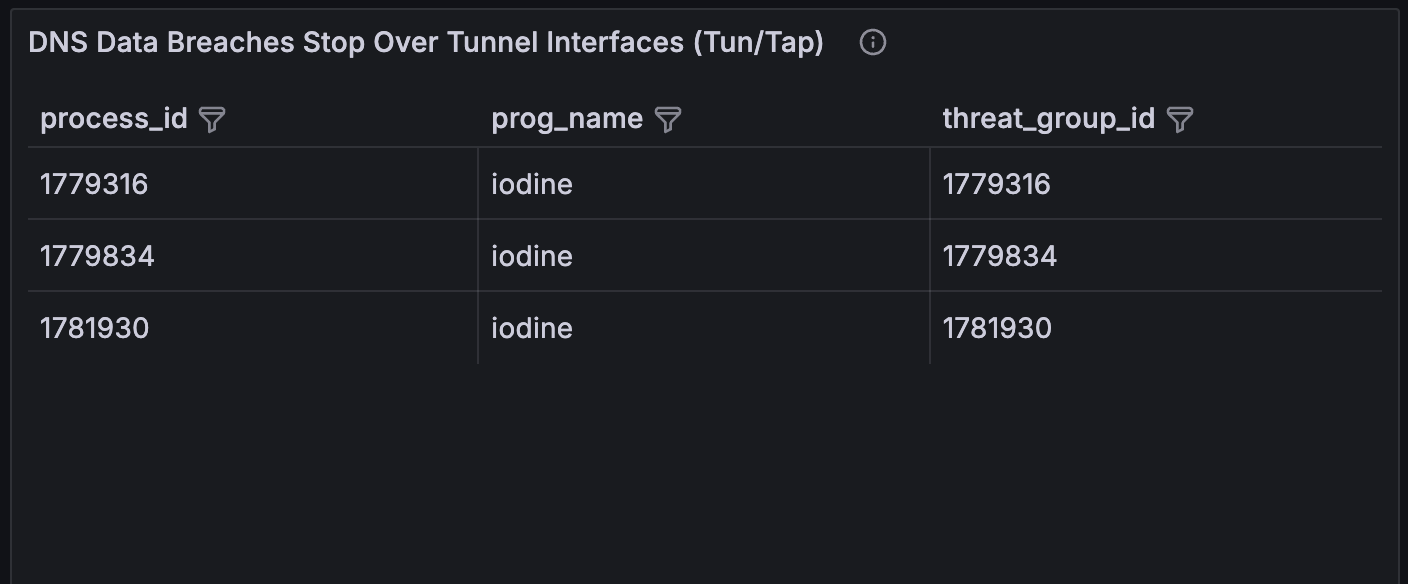
\includegraphics[width=\textwidth]{UWThesis/images/results/metrics/tunnel interface exfil metric.png}
    \caption{Tunnel Interface Exfiltration Metric}
  \end{subfigure}
  \hfill
  \begin{subfigure}[b]{0.48\textwidth}
    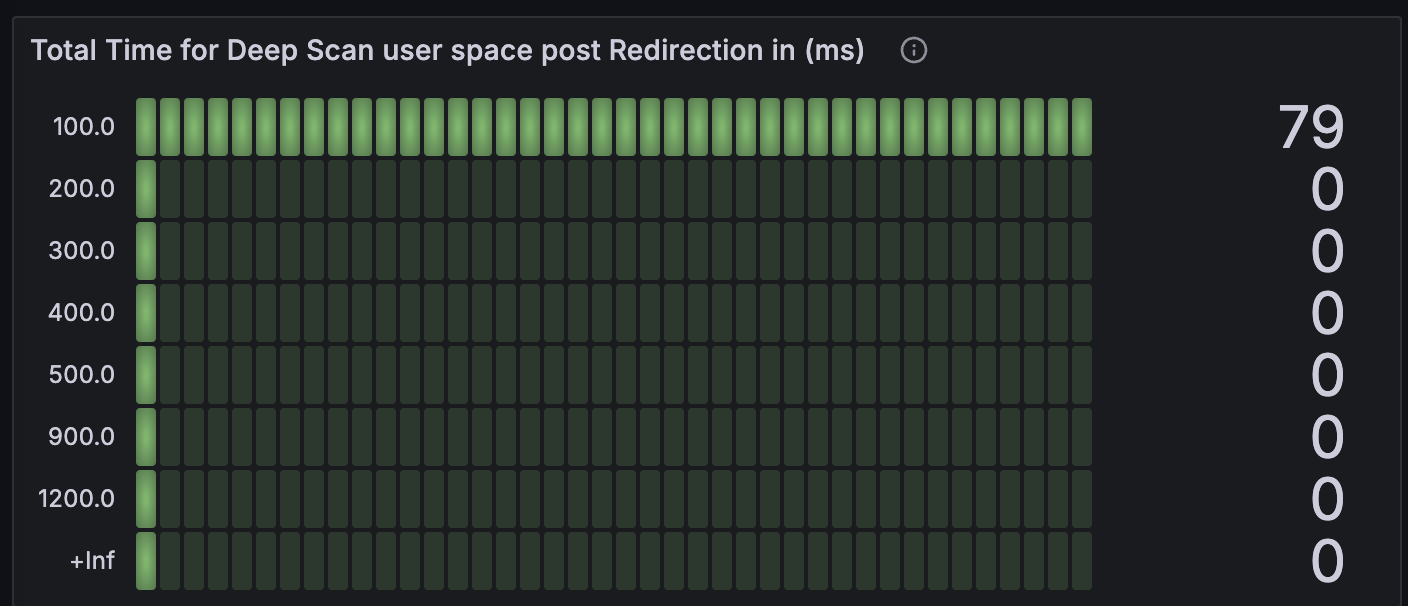
\includegraphics[width=\textwidth]{UWThesis/images/results/metrics/latency in active redirect mode.png}
    \caption{Latency in Active Redirect Mode}
  \end{subfigure}
  \caption{DNS Security Metrics: Exfiltration Attempts, Tunnel Behavior, Latency, and Detailed Packet Analysis}
  
  \vspace{0.8cm}
\end{figure}

\newpage
  % Row 3 (detailed image, full width)
  \begin{figure}
      \centering
      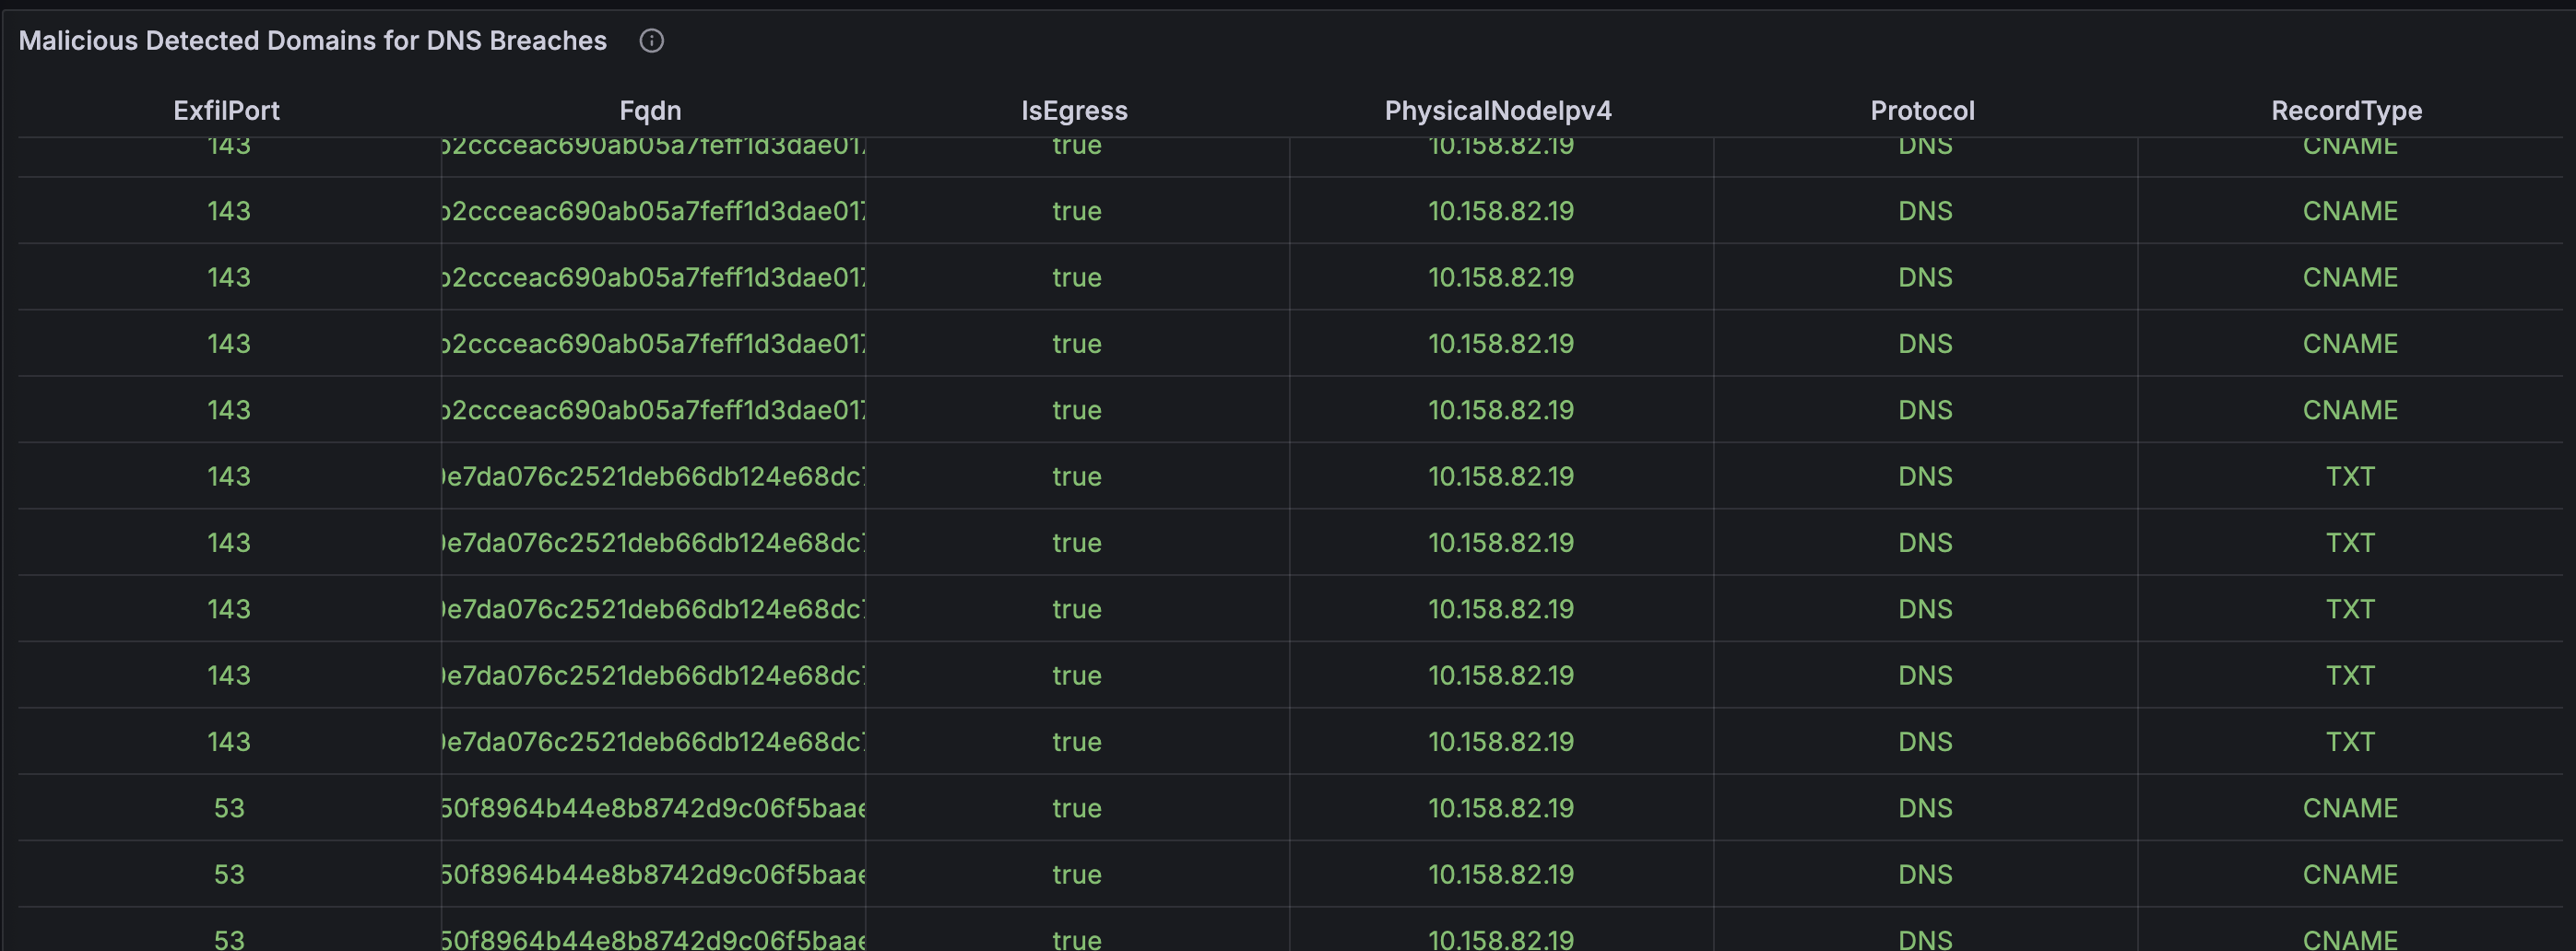
\includegraphics[width=0.5\linewidth]{UWThesis/images/results/metrics/dns_exfiltrated_packet_detailed_metrics.png}
      \caption{Caption}
      \label{fig:enter-label}
  \end{figure}








 
\bibliographystyle{plainnat}
\bibliography{UWThesis/uwthesis}


\end{document}
